	%--------------------------------------------------------------
% thesis.tex 
%--------------------------------------------------------------
% Corso di Laurea in Informatica 
% http://if.dsi.unifi.it/
% @Facolt� di Scienze Matematiche, Fisiche e Naturali
% @Universit� degli Studi di Firenze
%--------------------------------------------------------------
% - template for the main file of Informatica@Unifi Thesis 
% - based on Classic Thesis Style Copyright (C) 2008 
%   Andr\'e Miede http://www.miede.de   
%--------------------------------------------------------------
\documentclass[twoside,openright,titlepage,fleqn,headinclude,11pt,a4paper,BCOR5mm,footinclude]{scrbook}
\usepackage[pdftex,hyperfootnotes=false,pdfpagelabels,pagebackref]{hyperref}	%creates hyperlinks within the document.
\usepackage[pdftex]{graphicx}
\usepackage[dvipsnames]{xcolor}
\usepackage{microtype}
\usepackage[T1]{fontenc}
\usepackage[italian]{babel}	%typographic rules, hyphenations and special characters directly from keyboard
\usepackage[latin1]{inputenc}	%keyboard input encoding
\usepackage[square,numbers]{natbib}	%standard and non-standard bibliographic style files (BibTeX).  
\usepackage[fleqn]{amsmath}	%american mathematica society math symbols
\usepackage{amsfonts}	%collection is a set of miscellaneous TeX fonts 
\usepackage{amssymb}	%symbols
\usepackage{algorithmic}
\usepackage{algorithm}
\usepackage{bm}
\usepackage{url}%http URLs
\usepackage{breakurl}%http URLs that can be broken on multiple lines
\usepackage{soul}
\usepackage[framed]{ntheorem}
\usepackage{framed}
\usepackage{booktabs}
\usepackage{textcase}
\usepackage[automark]{scrpage2} 
\usepackage{titlesec}
%\usepackage{pstricks}
\usepackage[titles]{tocloft}
\usepackage{scrtime}
\usepackage{ifthen}
\usepackage{textcomp}
\usepackage{mparhack}
\usepackage{tabularx}
\usepackage{fixltx2e}
\usepackage{relsize}
\usepackage[smaller]{acronym}
\usepackage{caption}
\usepackage{remreset}
\usepackage{subfig}
\usepackage{listings}
\usepackage{ifpdf}
\usepackage{hyperref}
\usepackage[hyperpageref]{backref}
\usepackage[osf,sc]{mathpazo}
\usepackage{listings}
\usepackage{lstcustom}
\usepackage{bookmark}
\usepackage{setspace}
%\usepackage{index}
\usepackage[toc,page]{appendix}
\usepackage[titles]{tocloft}
\usepackage{multirow}
\definecolor{lightBlue}{rgb}{0.95,0.95,0.95}
%\lstset{language=Java, backgroundcolor=\color{SpringGreen}, basicstyle=\small, commentstyle=\color{green}}
\definecolor{javared}{rgb}{0.6,0,0} % for strings
\definecolor{javagreen}{rgb}{0.25,0.5,0.35} % comments\definecolor{javapurple}{rgb}{0.5,0,0.35} % keywords
\definecolor{javadocblue}{rgb}{0.25,0.35,0.75} % javadoc

%\definecolor{javabackground}{rgb}{0.25,0.35,0.55}
%\lstset{language=Java, backgroundcolor=\color{superLightBlue}, basicstyle=\small, commentstyle=\color{green}}
%\usepackage[acronym]{glossaries} % make a separate list of acronyms
%\makeglossaries
%--------------------------------------------------------------

\newcommand{\myTitle}{Metodi di Apprendimento Automatico per l'analisi in linea
della Deambulazione: Sviluppo e Validazione di un'applicazione per Smartphone\xspace}
\newcommand{\myEngTitle}{Machine Learning Methods for online Gait Analysis: Developement and Validation of a Smartphone Application}
%fr Machine Learning M�thodes d'analyse temps r�el la marche: D�veloppement et validation sur un Smartphone
%de Methoden des maschinellen Lernens f�r Real-Time-Ganganalyse: Entwicklung und Validierung auf einem Smartphone
%es Machine Learning m�todos de an�lisis de la marcha real de tiempo: Desarrollo y validaci�n en un Smartphone

% use the right myDegree option
%\newcommand{\myDegree}{Corso di Laurea in Informatica\xspace}
\newcommand{\myDegree}{	
	Corso di Laurea Specialistica in Scienze e Tecnologie 
	dell'Informazione\xspace}
\newcommand{\myName}{Ahadu Tsegaye\xspace}
\newcommand{\myProf}{Prof. Angelo Maria Sabatini\xspace}
\newcommand{\myOtherProf}{Prof. Maria Cecilia Verri\xspace}
%\newcommand{\mySupervisor}{Dott. Andrea Mannini\xspace}

%\newcommand{\myOtherProf}{Prof. Frasconi}
\newcommand{\myFaculty}{
	Facolt� di Scienze Matematiche, Fisiche e Naturali\xspace}
\newcommand{\myDepartment}{	Dipartimento di Sistemi e Informatica\xspace}
\newcommand{\myUni}{\protect{	Universit� degli Studi di Firenze}\xspace}
\newcommand{\myLocation}{Firenze\xspace}
\newcommand{\myTime}{Anno Accademico 2010-2011\xspace}
\newcommand{\myVersion}{\small \textcolor{red}{Revisione 5.0} \xspace} %last committed svn version.build
\newcommand{\myShortVersion}{\small \textcolor{red}{v5.0} \xspace}
%-----------------------------------------------------------\hypersetup{pdfstartview=FitW}
\hypersetup{pdfstartview=FitW}
%% Define a new 'leo' style for the package that will use a smaller font.
\makeatletter
\def\url@leostyle{%
  \@ifundefined{selectfont}{\def\UrlFont{\sf}}{\def\UrlFont{\small\ttfamily}}}
\makeatother
%% Now actually use the newly defined style.
\urlstyle{leo}
%--------------------------------------------------------------
\usepackage{dia-classicthesis-ldpkg} 
%--------------------------------------------------------------
% Options for classicthesis.sty:
% tocaligned eulerchapternumbers drafting linedheaders 
% listsseparated subfig nochapters beramono eulermath parts 
% minionpro pdfspacing
\usepackage[eulerchapternumbers,subfig,beramono,eulermath,parts]{classicthesis}
%--------------------------------------------------------------
\newlength{\abcd} % for ab..z string length calculation
% how all the floats will be aligned
\newcommand{\myfloatalign}{\centering} 
\setlength{\extrarowheight}{3pt} % increase table row height
\captionsetup{format=hang,font=small}
%--------------------------------------------------------------
% Layout setting
%--------------------------------------------------------------

%\usepackage{geometry}
%\geometry{
%	a4paper,
%	ignoremp,
%	bindingoffset = 1cm, 
%	textwidth     = 13.5cm,
%	textheight    = 21.5cm,
%	lmargin       = 3.5cm, % left margin
%	tmargin       = 3cm    % top margin 
%}
%--------------------------------------------------------------
%- Theorem Environments
%\theoremstyle{plain}% already by default
%---------------------------------------Begin Examples
\theoremstyle{change}
\theorembodyfont{\upshape}
\theoremsymbol{\ensuremath{\ast}}
\theoremseparator{}
\newtheorem{example}{Example}
%---------------------------------------End Examples
\newtheorem{exercise}{Exercise}
%\newtheorem{lemma}{Lemma}
\newtheorem{notation}{Notation}
\newtheorem{problem}{Problem}
\newtheorem{proposition}{Proposition}
\newtheorem{remark}{Remark}
\newtheorem{solution}{Solution}
\newtheorem{summary}{Summary}
%\newtheorem{theorem}{Theorem}

%\newtheorem{definizione}{Definizione}
%---------------------------------------Begin Definitions
\theoremstyle{plain}
\theoremsymbol{\ensuremath{\clubsuit}}
\theoremseparator{.}
\theoremprework{\bigskip\hrule}
\theorempostwork{\hrule\bigskip}
\newtheorem{definition}{Definizione}
%\newframedtheorem{definizione}{Definizione}
%\newshadedtheorem{definizione}{Definizione}
%-----------------------------------------End Definitions


\theoremstyle{marginbreak}
\theoremheaderfont{\normalfont\bfseries}\theorembodyfont{\slshape}
\theoremsymbol{\ensuremath{\diamondsuit}}
\theoremseparator{:}
\newtheorem{theorem}{Teorema} 
%--------------------------------------.For Lemmas:
\theoremstyle{changebreak}
\theoremsymbol{\ensuremath{\heartsuit}}
\theoremindent0.5cm
\theoremnumbering{greek}
\newtheorem{lemma}{Lemma} 

%--------------------------------------.For Examples:

%.For Proofs (note that theoremprework and theorempostwork are reset �
%proofs do not have lines above and below):
\theoremheaderfont{\sc}\theorembodyfont{\upshape}
\theoremstyle{marginbreak}
\theoremindent0.5cm
\theoremsymbol{\rule{1ex}{1ex}}
\newtheorem{dimostrazione}{Dimostrazione}

\newcommand{\TODO}[1]{[ {\em\marginpar{} \textcolor{blue}{TODO: #1} } ] }
\newcommand{\ERR}[1]{[ {\em\marginpar{} \textcolor{red}{ERR: #1} } ] }
\def\tm{\leavevmode\hbox{$\rm {}^{TM}$}}

\renewcommand\lstlistingname{Codice}
\renewcommand\lstlistlistingname{Codice}
\def\lstlistingautorefname{Cod.}


\renewcommand{\appendixtocname}{Appendici}
\renewcommand{\appendixpagename}{Appendici}

%\newglossaryentry{sample}{name={sample},description={a sample entry}}
%\newacronym[\glsshortpluralkey=cas,\glslongpluralkey=contrived acronyms]{aca}{aca}{a contrived acronym}

%--------------------------------------------------------------
%--------------------------------------------------------------
\makeatletter
\renewcommand{\@pnumwidth}{3em}
%\renewcommand{\linewidth}{3em}
\renewcommand{\@dotsep}{4.5}
\def\l@chapter{\@dottedtocline{0}{2em}{1em}}
\def\l@section{\@dottedtocline{1}{4em}{1.8em}}
\def\l@subsection{\@dottedtocline{2}{6em}{2.4em}}
\def\l@subsubsection{\@dottedtocline{3}{8em}{3.6em}}
\makeatother
%%% Aesthetic spacing redefines that look nicer to me than the defaults.
%
%\setlength{\cftbeforechapskip}{2ex}
%\setlength{\cftbeforesecskip}{0.5ex}
%
%
\renewcommand{\cftpartpresnum}{PARTE  }
\renewcommand{\cftpartfont}{\hfill\Large\bfseries\hfill}

%\renewcommand{\cftchapfont}{\bfseries}
%\renewcommand{\cftchapleader}{\bfseries\cftdotfill{\cftchapdotsep}}
%\renewcommand{\cftchappagefont}{\bfseries}
%\renewcommand{\cftchappresnum}{CAP}
%\renewcommand{\cftchapaftersnum}{:}
%\renewcommand{\cftchapaftersnumb}{\\}

%}
%\makeindex
\onehalfspacing
\begin{document}
%%English words --- to Italian (if possible)

% la migliore soluzione � mettre la parola in inglese, traduzione ed un acronimo, poi uso solo l'aconimo


% Terms from Chinesiology
\newcommand{\HEELSTRIKE}{ $Contatto\_\-Del\_\-Tallone$}
\newcommand{\HEELOFF}{ $Tallone\_\-Alzato$}
\newcommand{\FOOTFLAT}{ $Piede\_\-A\_\-Terra$ }
\newcommand{\TOEOFF}{ $Piede\_\-Alzato$ }
\newcommand{\STANCE}{ $Fase\_\-A\_\-Terra$ }
\newcommand{\SWING}{ $Fase\_\-In\_\-Aria$ }
\newcommand{\INITIALSWING}{ $Prima\_\-Fase\_\-In\_\-Aria$ }
\newcommand{\TERMINALSWING}{ $Ultima\_\-Fase\_\-In\_\-Aria$ }
\newcommand{\LOADRESPONSE}{ $Risposta\_\-Al\_\-Carico$ }
\newcommand{\MIDSTANCE} { $Fase\_\-Intermedia\_\-A\_\-Terra$ }
\newcommand{\TERMINALSTANCE} { $Ultima\_\-Fase\_\-A\_\-Terra$ }
\newcommand{\PRESWING}{ $Pre\_\-Aerea$ }

% cs
\newcommand{\OFFLINE}{ in differita }
\newcommand{\ML}{ Apprendimento Automatico }
\newcommand{\PR}{ Pattern Recognition }
\newcommand{\HMM}{ Modelli di Markov a Stati Nascosti }
%verificare
\newcommand{\ONLINE}{ in tempo reale }
\newcommand{\REALTIME}{ in tempo reale }
\newcommand{\THRESHOLD}{ valori soglia }
\newcommand{\PERFORMANCE}{ performance }
\newcommand{\OUTPUT}{ output }
\newcommand{\INTPUT}{ input }

%ML
\newcommand{\TRAININGSET}{ Training Set }
\newcommand{\TARGET}{ target }
\newcommand{\LEFTTORIGHT}{ left to right }


% instruments
\newcommand{\MOTIONCAPTURE}{ ripresa del movimento }
\newcommand{\SP}{ Smartphone }
\frenchspacing
\raggedbottom
\pagenumbering{roman}
\pagestyle{plain}
%--------------------------------------------------------------
% Frontmatter
%--------------------------------------------------------------
\frontmatter
%--------------------------------------------------------------
% titlepage.tex (use thesis.tex as main file)
%--------------------------------------------------------------
\begin{titlepage}
	\begin{center}
   	\large
      \hfill
      \vfill
      \begingroup
			\spacedallcaps{\myUni} \\ 
			\myFaculty \\
			\myDegree \\ 
			\vspace{0.5cm}
         
\includegraphics[scale=.065]{logo/unifi}\\
         \vspace{0.5cm}    
         Tesi di Laurea    
      \endgroup 
      \vfill 
      \begingroup
      	\color{RoyalBlue}\spacedallcaps{\myTitle} \\ \bigskip
      \endgroup
      \spacedlowsmallcaps{\myName}
      \vfill        
			\begin{flushleft}
			\hspace{2.5cm} Relatore \hspace{.6cm}\textit{\myProf}\\ 
			      \vspace{0.3cm}
			\hspace{2.6cm}Co-Relatore\hspace{.3cm}\textit{\myOtherProf}\\
			\end{flushleft}
      \vfill
      \myTime\\
      \hspace{.5cm}
      \myVersion
      \vfill                      
	\end{center}        
\end{titlepage}   
%--------------------------------------------------------------
% back titlepage
%--------------------------------------------------------------
   \newpage
	\thispagestyle{empty}
	\hfill
	\vfill
	\noindent\myName: 
	\textit{\myEngTitle}, 
	\myDegree \textcopyright\ \myTime-\myShortVersion

%--------------------------------------------------------------
% back titlepage end
%--------------------------------------------------------------
\renewcommand\contentsname{Indice}
\addtocontents{toc}{~\hfill\textbf{Pagina}\par}
\tableofcontents

%\makeatletter \renewcommand{\@dotsep}{10000} \makeatother
%\listoftables
%\makeatletter \renewcommand{\@dotsep}{4.5} \makeatother
%\listoffigures


\pagestyle{scrheadings}
%--------------------------------------------------------------
% Mainmatter
%--------------------------------------------------------------
\mainmatter
\cleardoublepage 
\pagenumbering{arabic}

\chapter{Sommario}
%\myChapter{Sommario}

In questo lavoro si affronta il problema dell'analisi in linea della deambulazione umana mediante metodi di apprendimento automatico e lo sviluppo di un'applicazione per \textit{Smartphone Android}.\\
Una HMM (\textit{Hidden Markov Model}) a quattro stati addestrata in differita su segnali giroscopici provenienti da sessioni di cammino e corsa su un tappeto rullante a diverse velocit� ed inclinazioni, viene usata per segmentare in linea le fasi del cammino grazie ad una versione modificata dell'algoritmo di decodifica di Viterbi.\\
Il giroscopio usato � contenuto in una IMU (\textit{Inertial Measurement Unit}) collocato sul collo del piede ed orientato con l'asse sensibile sul piano mediale laterale.\\
L'applicazione per \textit{Smartphone} permette di controllare la IMU via \textit{Bluetooth}, nonch� di segmentare e visualizzare in linea il segnale giroscopico relativo a deambulazione. \\
La validazione del sistema viene fatta stimando la distanza percorsa calcolata da dati (cadenza e velocit�) ottenuti in sessioni di cammino su tappeto rullante in laboratorio, e confrontandola con la distanza misurata mediante GPS in sessioni di cammino all'aperto, in condizioni non controllate.\\
%I risultati sono ... 

\addtocontents{toc}{\protect\mbox{}\protect\hrulefill\par}
\addtocontents{toc}{\protect\mbox{}\protect\hrulefill\par}
\addtocontents{toc}{\cftpagenumbersoff{part}}
\part{Stato dell'arte}

\chapter{Introduzione}
%\myChapter{Introduzione}

%-------------------	Descrizione del problema -------------------------------
Ipotesi: \textit{� possibile costruire un sistema intelligente e portatile in grado di riconoscere (classificare) e analizzare i movimenti di un individuo e di fornirne in linea (vedi appendice \ref{sec:real_time_sys}) informazioni a riguardo}.\\

Il problema del riconoscimento (classificazione) di una generica attivit� motoria umana � irrisolto ed estremamente complesso visto il numero esorbitante di parametri coinvolti.
In questo lavoro viene affronta l'analisi di una singola attivit� nota: la deambulazione entro un intervallo di velocit� e pendenza del terreno.

Nello specifico il problema � quello dell'individuazione in linea delle tempistiche di eventi che costituiscono una deambulazione normale come studiato dalla Chinesiologia (vedi capitolo \ref{cap:chinesiologia}). Tale problema � noto come \emph{problema della segmentazione automatica ed in linea della deambulazione umana}.\\

%------------------  Motivazioni del problema Perch� si pone?--------------------------------
La soluzione del problema della segmentazione avrebbe risvolti immediati nella Medicina riabilitativa per la diagnosi e/o assistenza a persone con problemi di deambulazione, nella Robotica e Computer Grafica per la emulazione/simulazione della deambulazione umana, nel mondo dello sport agonistico per l'apprendimento di specifiche tecniche motorie.\\

%---------------------� gia stato affrontato? 
Il problema della segmentazione � stato ampiamente affrontato nella letteratura scientifica (letteratura biomedica, biomeccanica, ingegneria medica) con svariate combinazioni di materiali e metodi. 

Per quanto riguarda i materiali, sono state proposte soluzioni basate sull'osservazione diretta di un fisiatra; basate sulla stereofotogrammetria, sistemi di telecamere ad emissione di luce infrarossa e marcatori riflettenti; basate su strumenti inerziali, sensori fisici: accelerometri, giroscopi, elettromagnetometri. 
\begin{figure}
	\centering
	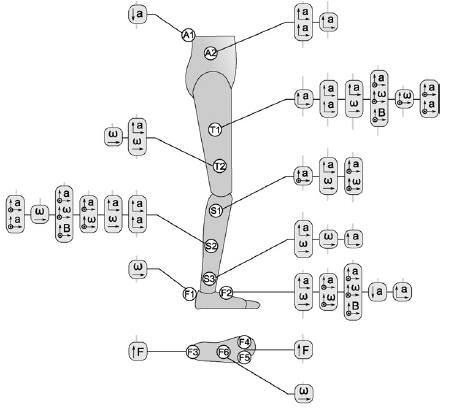
\includegraphics[width=1\textwidth]{imgs/sensorOnBodyLocations.jpg}
	\caption{Schema riassuntivo dei posizionamenti di diversi sensori su diverse parti del corpo, usati in letteratura. Immagine adattata da \cite{gait_event_detection_analysis}}
	\label{fig:sensorOnBodyLocations}
\end{figure}
Questi ultimi sono stati usati in diverse combinazioni, numero e disposizione sul corpo (vedi immagine \ref{fig:sensorOnBodyLocations}).\\ 

Per quanto riguarda i metodi, sono state proposte soluzioni di tipo cinematico basato sullo studio delle forze che agiscono sul corpo nella deambulazione; di tipo analitico (studio di funzioni e curve) sui segnali di sensori inerziali; alle Macchine a stati finiti per lo studio di sequenze temporali, e pi� di recente all'Apprendimento Automatico (Reti Neurali, Logica Fuzzy) per la capacit� di astrarre sulle variazioni dei singoli individui \cite{gait_event_detection_analysis}.

% -------------------------------� stato gia stato risolto? 
\ERR{Nonostante il vasto numero di lavori, non � ancora stata data una soluzione soddisfacente al problema. 
Tutti i metodi proposti peccano di dipendenza dagli strumenti che usano, vale a dire che variando questi ultimi, variano le prestazioni dei metodi e di dipendenza dai soggetti sui quali vengono fatti gli esperimenti.}\TODO{citazione}\\

%------------------------- Come voglio affrontare il problema? 
La scelta dell'utilizzo delle HMM � giustificata dai seguenti motivi. 
Le HMM (vedi appendice \ref{cap:hmm}) sono uno strumento stocastico di riconoscimento di schemi (\textit{Stochastic Pattern Recognition}) usato in campi come il riconoscimento vocale \cite{tutorial_hmm_application_speech_recognition} e lo studio della visione artificiale per il riconoscimento gestuale \cite{HMM_gesture_recognition}. Uno studio dimostra il potenziale delle HMM per la segmentazione della deambulazione equina \cite{stride_segmentation_technique_hmm}. \\

Inoltre vi sono studi che usano le HMM come struttura gerarchica per affrontare il problema della classificazione di attivit� umane \cite{human_physical_activity_classification_ml, spatio_temporal_params_gait_gyr}. Per sviluppi futuri, del lavoro qui presentato, nella direzione della risoluzione del problema della classificazione, gli studi citati sono a favore dell'utilizzo delle HMM.
 % use \myChapter command instead of \chapter
\chapter{Cenni alla Chinesiologia}
%\myChapter{Cenni alla Chinesiologia}
\label{cap:chinesiologia}
$\kappa\iota\nu\eta\sigma\iota\varsigma \quad (kin\bar{e}sis)$:  mobilit�,\\
$\lambda o\gamma \iota \alpha \quad (logia)$: studio di\\


%The study of the principles of mechanics and anatomy in relation to human movement.
Studio dei principi su cui si fondano la meccanica e l'anatomia del movimento umano. 


\begin{flushright}
\emph{www.merriam-webster.com} \cite{merriam-webste_Online}
\end{flushright}

\vspace{1cm}

La Chinesiologia studia il movimento umano sotto diversi aspetti: biomeccanico, del controllo motorio e della psicologia del moto.\\
L'approccio biomeccanico \cite{Hall_basic_biomechanics} consiste nell'applicazione dei principi della Meccanica allo studio di organismi viventi: principalmente propriet� fisiche di materiali biologici, segnali biologici, modellazioni e simulazioni biomeccaniche.

Per restringere l'ambito, noi ci concentriamo sulle interazioni biomeccaniche dell'apparato locomotore (scheletro e muscoli).
La branca della Meccanica Classica (vedi Appendice \ref{meccanica_classica}) 
che viene utilizzata dalla Biomeccanica � la Cinematica \cite{Encyclopedia_Britannica_online}
che si occupa di descrivere la posizione ed il moto di oggetti nello spazio, senza riferimento alle forze o masse coinvolte (vale a dire alle cause e agli effetti di tale moto). 

\section{Analisi dei movimenti del corpo umano}
Per un trattamento rigoroso dei movimenti del corpo umano, � necessario stabilire dei piani di riferimento, lungo i quali collocare le diverse parti del corpo (vedi Figura \ref{fig:HumanBodySPL}).

\begin{figure}
	\centering
		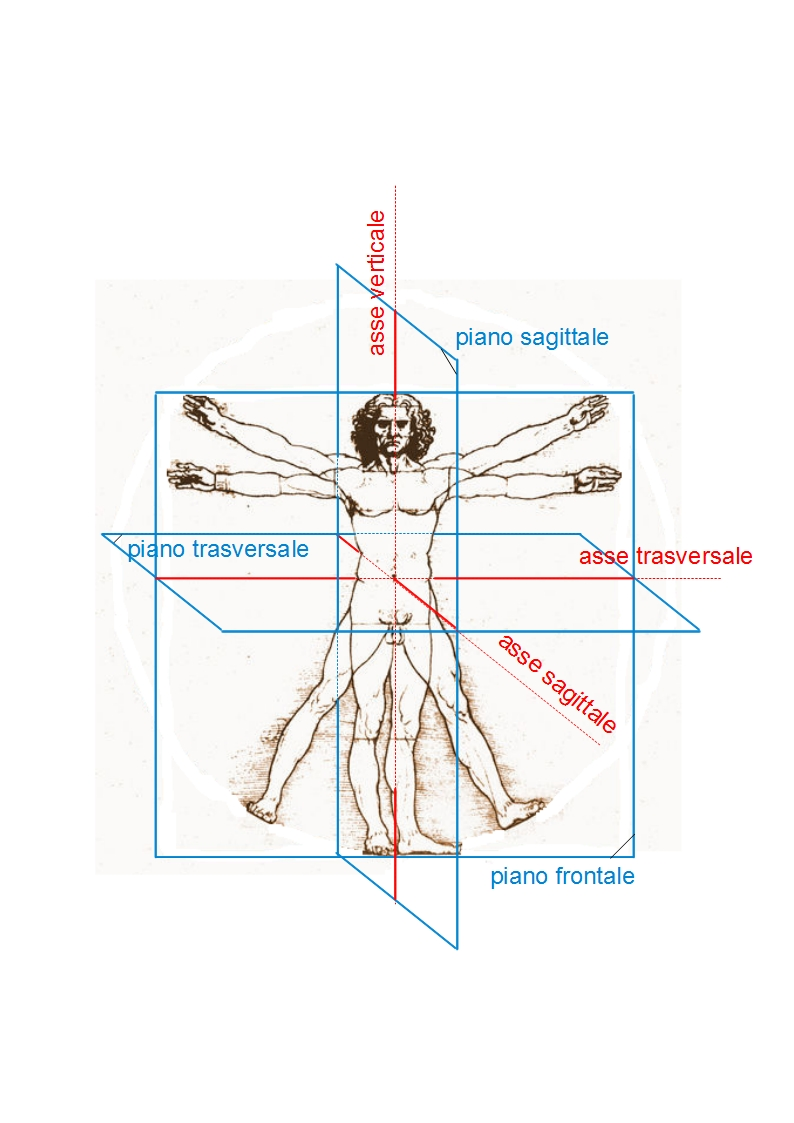
\includegraphics[width=1\textwidth]{imgs/Human_body_by_Da_Vinci-SPL.jpg}
	\caption{Piani ed assi che tagliano il corpo umano nelle tre dimensioni spaziali, utilizzate per definirne il movimento.}
	\label{fig:HumanBodySPL}
\end{figure}

\begin{definition}[Piani che tagliano il corpo umano]
I movimenti del corpo umano vengono descritti in riferimento a tre piani:
	\begin{enumerate}
		\item \textbf{Frontale o Coronale}:  piano verticale che divide il corpo in parte anteriore e posteriore.
		\item \textbf{Sagittale}: piano verticale che divide il corpo in parte sinistra e destra.
		\item \textbf{Trasversale o Orizzontale}: piano orizzontale che divide il corpo in parte superiore ed inferiore. 
	\end{enumerate}
\end{definition}
Ad esempio la deambulazione o corsa avviene principalmente lungo il piano sagittale, sollevare le braccia lateralmente comporta un movimento sul piano frontale, mentre la rotazione della testa per guardarsi intorno avviene principalmente lungo il piano trasversale. 


\section{L'andatura durante la deambulazione}
Viene definita Andatura (\textit{Gait}) la sequenza di movimenti degli arti inferiori che un animale compie su una superficie solida durante la locomozione \cite{Herbrand_gait}. Gli animali possiedono diverse forme di andatura che scelgono in base alla velocit�, ed al terreno ed ad altre variabili. \\
La Deambulazione (o Camminata) � una delle principali forme di andatura degli animali aventi arti inferiori ed avviene tipicamente a velocit� inferiore a quelle della Corsa (che a sua volta � una forma di locomozione).  
\begin{definition}[Deambulazione Normale]
\label{deambulazione_normale}
Una Deambulazione normale (negli esseri umani) � composta di due macro fasi per ciascun piede: 
\begin{enumerate}
	\item Fase di appoggio (\textit{Stance}), in cui il piede supporta tutto il peso del corpo e
	\item Fase in aria (\textit{Swing}), in cui il piede � in aria e porta avanti il baricentro del corpo, mentre il peso del corpo � sull'altro piede.
\end{enumerate}
I due arti inferiori sono sempre alternativamente nelle due fasi e per circa il 25\% del tempo sono in contatto simultaneo con il pavimento.
\end{definition}


\section{Breve storia dello studio della deambulazione umana}
Un primissimo contributo allo studio dell'andatura umana � stato dato dai  fratelli Wilhelm Weber, fisico, e Eduard Weber, anatomista. I Weber, nel loro libro \emph{The Mechanics of Human Motions} \cite{Weber_mechanics_human_motion}, pubblicato nel 1836, definiscono e misurano per la prima volta la durata delle fasi della Deambulazione Normale (vedi Definizione \ref{deambulazione_normale}), usando solamente un cronometro ed un telescopio con una scala.\\
Un grande contributo a questo campo � stato dato dal fisiologo francese $\grave{E}$tienne Jules Marey, che nel 1873 pubblic� il trattato  \emph{Animal Mechanism: a Treatise on Terrestrial and Aerial Locomotion} dove con l'uso di scarpe a camera d'aria collegate a un registratore e della \textit{Cronofotografia Geometrica}\footnote{pi� riprese fotografiche vengono impresse sulla stessa fotografia, in modo che possa essere ripresa una sequenza di azioni della persona. Si tratta di un antenato della cinepresa.} e con l'uso di soggetti vestiti con abiti aderenti e neri con bottoni di metallo e strisce riflettenti, riusc� a misurare la durata del contatto del piede con il suolo, durante la camminata in piano, su un terreno regolare. Inoltre egli introdusse il concetto dell'efficienza energetica del movimento.\\
Il fotografo inglese Edward Muybridge, nel 1887 con l'uso della fotografia seriale, con 48 fotocamere elettriche sincronizzate riusc� a catturare la fase in volo di un cavallo al galoppo.\\
L'anatomista tedesco Wilhelm Braune, ed il matematico tedesco Otto Fisher, negli anni 1890, con l'uso di un sistema a 4 fotocamere, un tubo luminoso attaccato al corpo ripreso ed un sistema di riferimento rettangolare, riuscirono a analizzare per la prima volta l'andatura in 3D ed a stabilire i metodo per il calcolo dei parametri meccanici dello stesso. \\
Nel 1938 Elftman e 20 anni dopo Frankel diedero grossi contributi agli studi di tipo cinetico sul passo normale e patologico\footnote{passo affetto da una qualunque tipo di deformazione rispetto al passo normale}.\\
M.P. Murray, negli anni '60, con l'uso della fotografia a luce interrotta e pi� tardi con il sistema 3D, diede dei contributi allo studio cinetico in pazienti normali e patologici. \\
J Perry con l'uso di goniometri elettronici monoassiali ha sviluppato un nuovo sistema di terminologie per l'andatura sia normale che patologica. 

\section{Ciclo di deambulazione}
L'unit� di base per la descrizione dell'andatura nella deambulazione � il ciclo di andatura (\textit{Gait Cycle}) (vedi Figura \ref{fig:CicoloDelPasso}). Si tratta della sequenza di azioni compiute dal corpo dall'istante dell'impatto di un tallone a terra fino al impatto successivo dello stesso tallone. Il ciclo di andatura ha una durata compresa nell'intervallo di [0.5-2] secondi, in base alla velocit�. Il ciclo di andatura � suddiviso in due fasi: una di appoggio, in cui il piede � a contatto con il terreno, ed una aerea. 
\begin{figure}[h]
	\centering
		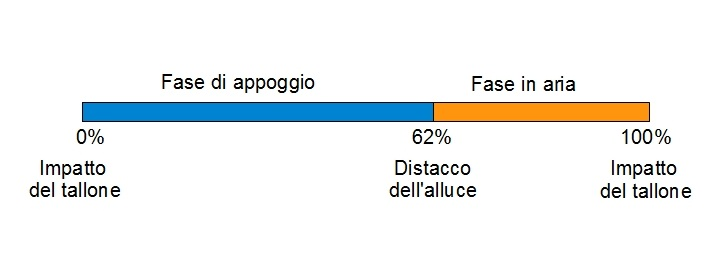
\includegraphics[width=0.95\textwidth]{imgs/CicoloDelPasso.jpg}
	\caption{Ciclo completo di andatura }
	\label{fig:CicoloDelPasso}
\end{figure}

%La fase di appoggio (dal contatto del tallone al distacco dell'alluce dal terreno) viene ulteriormente suddivisa in tre sottofasi: 
%\begin{enumerate}
%	\item contatto iniziale;
%	\item appoggio intermedio (detta anche fase di risposta al carico);
%	\item fase propulsiva (o di contatto finale).
%\end{enumerate}
 

%\section{Gait Cycle}
\begin{figure}[h]
	\centering
		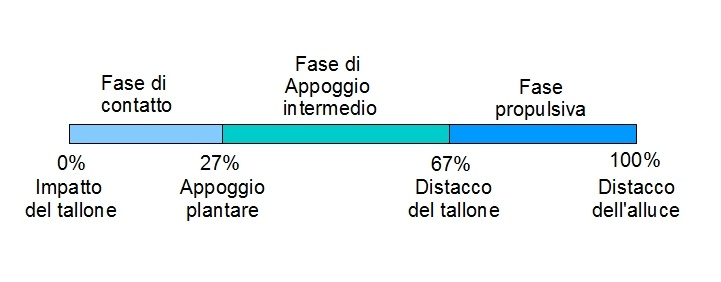
\includegraphics[width=0.95\textwidth]{imgs/CicoloDelPassoAppoggio.jpg}
	\caption{Fase di appoggio}
	\label{fig:CicoloDelPassoAppoggio}
\end{figure}


Le due fasi possono essere ulteriormente suddivise. In queste vi sono eventi che determinano l'inizio e la fine di una fase. Per definizione un ciclo di deambulazione inizia e termina con la fase HS (\textit{Heel Strike}) ovvero impatto del tallone con il suolo. All'evento HS cui segue la fase LR (\textit{Load Response}) fase di risposta al carico, ovvero il peso del corpo si sposta per gran parte sul piede avanti. A termine della fase LR, si verifica l'evento FF (\textit{Foot Flat}) appoggio plantare, in cui il piede avanti si trova piatto sul suolo. L'evento FF � seguito dalla fase MS (\textit{Mid Stance}) fase di appoggio intermedio in cui il corpo si spinge in avanti ed il piede indietro si innalza da. L'evento che termina la fase MS � HO (\textit{Heel Off}) distacco del tallone, che indica la transizione ad una transizione tra la fase TS (\textit{Terminal Stance}) propulsione ed una breve fase nota come PSw (\textit{Pre Swing}) pre-distacco che precede la fase in aria. In questa transizione il corpo viene nuovamente spinto in avanti, e tale spinta provoca l'ultimo evento della fase di appoggio del piede ovvero TO (\textit{Toe Off}) distacco dell'alluce. Dopo TO inizia la fase in aria del piede. In questa fase il piede in aria si porta davanti al piede portante permettendo cos� l'inizio di un nuovo ciclo di deambulazione. Anche la fase in aria pu� essere suddivisa in tre fasi: ISw (\textit{Initial Swing}) propulsione iniziale in cui l'arto viene accelerato, MSw (\textit{Mid Swing}) propulsione mediale in cui l'arto per aria sorpassa quello a terra ed infine TSw (Terminal Swing) decelerazione, in preparazione per l'atterraggio, ovvero l'evento iniziale HS. 
 

\begin{table}%
\begin{tabular}{|m{5cm}|m{5cm}|m{.5cm}}
\cline{1-2}
\textsc{Evento} & \textsc{Fase}&\\
\cline{1-2}
\cline{1-2}
\textbf{HS} - impatto del tallone&&\\
\cline{2-2}
& LR - risposta al carico&\multirow{6}{*}{\rotatebox{90}{Fase di appoggio}}\\
\cline{2-2}
\textbf{FF} - appoggio plantare &&\\
\cline{2-2}
& MS - appoggio intermedio&\\
\cline{2-2}
\textbf{HO} - distacco del tallone &&\\
\cline{2-2}
& TS - propulsione&\\
\cline{2-2}
& Psw - pre distacco&\\
\cline{2-2}
\textbf{TO} - distacco dell'alluce &&\\
\cline{1-2}
& ISw - accelerazione&\multirow{3}{*}{\rotatebox{90}{Fase in aria}}\\
\cline{2-2}
& MSw - superamento&\\
\cline{2-2}
& TSw - decelerazione&\\
\cline{2-2}
\textbf{HS}&&\\
\cline{1-2}
\end{tabular}
\newline
\caption{Ulteriori suddivisioni del cammino in eventi e fasi.}
\label{fasi_del_cammino}
\end{table}




\subsection{Confronto fra Falcata (\textit{Stride}) e Passo (\textit{Step})}

La falcata, che va dal impatto del tallone con il suolo fino al successivo contatto dello stesso piede, � sinonimo di ciclo di andatura (\textit{Gait Cycle}), mentre il passo comincia dal impatto di un tallone e termina al impatto dell'altro tallone. Una falcata coincide esattamente con due passi (vedi Figura \ref{fig:AndaturaConfrontoPasso}).
\begin{figure}[h]
	\centering
		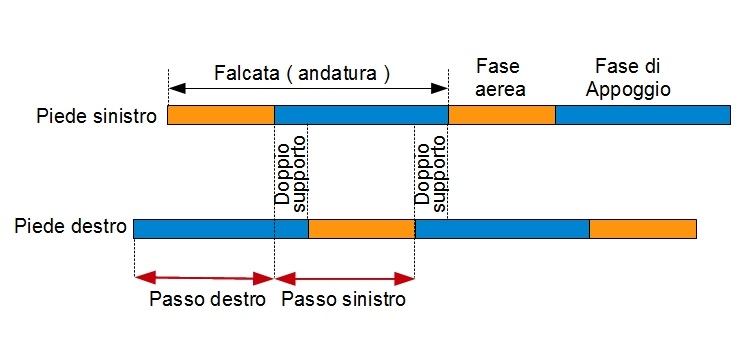
\includegraphics[width=0.95\textwidth]{imgs/AndaturaConfrontoPasso.jpg}
	\caption{Andatura e Passo a confronto}
	\label{fig:AndaturaConfrontoPasso}
\end{figure}

\section{Parametri che descrivono lo schema \textit{pattern} della deambulazione}
I parametri della deambulazione sono suddivisi fra quelli temporali e spaziali. Come � chiaro dal nome, i parametri temporali sono quelli misurabili in unit� temporali ovvero le durate di eventi (vedi Tabella \ref{parametri_temporali}), mentre i parametri spaziali sono quelli misurabili in unit� spaziali (vedi Tabella \ref{parametri_spaziali}).
%\begin{wraptable}{r}[-9mm]{0.30\textwidth}
\begin{table}[h]%
\begin{tabular}{|p{3cm}|p{2cm}|p{5cm}|}
\hline
\textsc{nome parametro} & \textsc{unit� di misura} & \textsc{descrizione}\\
\hline
\hline
Andatura &(sec)& durata di un completo ciclo di andatura\\
\hline
Passo &(sec)& durata di un completo passo sinistro o destro\\
\hline
Contatto &(sec, \%)& durata del periodo in cui i piedi rimangono a contatto con il terreno\\
\hline
Contatto a piede singolo &(sec, \%)&durata del periodo in cui solo un piede rimane a contatto con il terreno\\
\hline
Doppio contatto &(sec, \%)& durata del periodo in cui entrambi piede rimangono contemporaneamente a contatto con il terreno\\
\hline
Fase aerea &(sec, \%)& durata del perodo in cui il piede � in aria\\
\hline
\end{tabular}
\newline
\caption{Parametri temporali}
\label{parametri_temporali}
\end{table}
%\end{wraptable}


\begin{table}%
\begin{tabular}{|p{3cm}|p{2cm}|p{5cm}|}
\hline
\textsc{nome parametro} & \textsc{unit� di misura} & \textsc{descrizione}\\
\hline
\hline
Lunghezza dell'andatura &(cm)& distanza tra due punti di impatto successivi dello stesso tallone\\
\hline
Lunghezza del passo &(cm)& distanza tra due punti di impatto successivi di talloni opposti\\
\hline
Larghezza del passo &(cm)&distanza laterale tra due punti di impatto successivi di talloni opposti\\
\hline
Angolo del piede &(gradi)& angolo tra il collo del piede e lo stinco \\
\hline
\end{tabular}
\newline
\caption{Parametri spaziali}
\label{parametri_spaziali}
\end{table}

\begin{table}%
\begin{tabular}{|p{3cm}|p{2cm}|p{5cm}|}
\hline
\textsc{nome parametro} & \textsc{unit� di misura} & \textsc{descrizione}\\
\hline
\hline
Cadenza & (passi/ min) & numero di passi per unit� di tempo oppure RPM (\textit{Revolutions Per Minute})\\
\hline
Velocit� del passo &(m/s) & numero di metri percorso al secondo \\
\hline
\end{tabular}
\caption{Parametri di velocit�}
\label{parametri_velocit�}
\end{table}
\chapter{Lo stato dell'arte}
%\myChapter{Lo stato dell'arte}
Il mondo scientifico che si � confrontato con il problema della segmentazione della deambulazione, e pi� in generale sull'analisi della deambulazione ed individuazione delle sue varie fasi, � molto vasto e variegato. 
Per avere una visuale completa sul panorama di ricerca in questo ambito, si pu� suddividere lo stato dell'arte per materiali e metodi usati. 


\section{Materiali} 
Per materiali si intende tutto l'arsenale fisico, usato per captare, misurare e raccogliere dati riguardanti la deambulazione. I materiali possono, a loro volta, essere suddivisi in quelli che permettono di fare misure dirette dei parametri della deambulazione, ovvero spostamento, velocit� e accelerazione sia lineare che angolare di arti e articolazioni; e quelli che permettono di fare misurazioni indirette della deambulazione con sistemi di tracciamento del movimento.

\subsection{Osservazione diretta del paziente} Il fisiatra � figura medica che si occupa di diagnosi, terapia e riabilitazione di persone con problemi di limitazioni di attivit�, in questo caso motorie. Un fisiatra � in grado, ad occhio nudo, di fare considerazioni importanti sulla deambulazione di un individuo. Ad esempio lo studio \cite{ambulatory_devices_gait_disorders} dimostra che un fisiatra � in grado di consigliare ad anziani con problemi cronici di deambulazione (ovvero che non possono essere trattati ne medicalmente ne chirurgicamente), il tipo di supporto da utilizzare per facilitare l'attivit�. Lo studio dimostra anche che l'utilizzo di dispositivi per misure accurate dei parametri della deambulazione aiutano il fisiatra a scegliere il supporto di deambulazione adeguato, nonch� un addestramento all'uso dello stesso consono al tipo di problema deambulatorio del paziente. 

\subsection{Stereofotogrammetria} 
\label{sec:stereofotogrammetria}
Metodologia di ricostruzione virtuale di oggetti ed del loro moto in tre dimensioni basato sulla sovrapposizione di immagini riprese da pi� telecamere posizionate intorno all'oggetto (vedi Figura \ref{fig:vicon}). Sull'oggetto vengono posizionati dei marcatori riflettenti (vedi Figura \ref{fig:markers}) che sono i punti di riferimento per le telecamere. I marcatori sono dei bulbi sferici in plastica retroriflettenente (superficie che riflette la luce alla sua sorgente minimizzando l'angolo di riflessione quindi minimizzando anche la dispersione di luce) di circa 14mm di diametro, attaccati ad una superficie quadrata della stessa dimensione, alle quali viene applicato del nastro biadesivo, mediante il quale vengono incollate sulla parte del corpo che vuole studiare. La ricostruzione del moto dell'oggetto avviene mediante il calcolo degli spostamenti relativi dei marker. Il sistema commerciale utilizzato in questo lavoro � Vicon\tm \cite{vicon.com}.
\begin{figure}
	\centering
		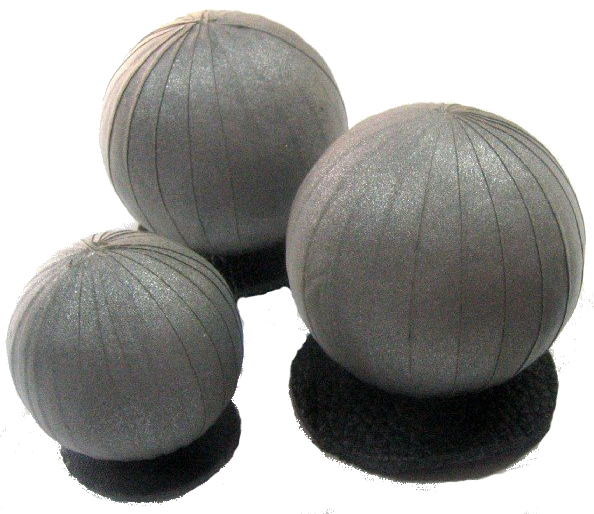
\includegraphics[width=.4\textwidth]{imgs/ReflectiveMarker.jpg}
	\caption{Marcatori riflettenti per il sistema Vicon\tm.}
	\label{fig:markers}
\end{figure}

\begin{figure}
	\centering
		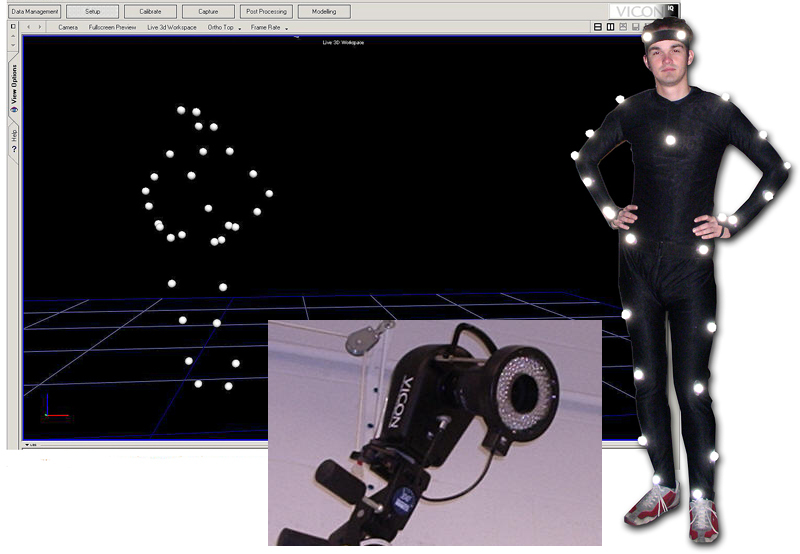
\includegraphics[width=1\textwidth]{imgs/viconMotionCapture.jpg}
	\caption{Strumentazione del sistema stereofotogrammetrico Vicon\tm}
	\label{fig:vicon}
\end{figure}


\subsection{Sensori}
In letteratura vengono usati diversi tipi di sensori, dai quali segnali vengono estratti i parametri della deambulazione. 

%%%%% forza + mag %%%%%%%%%%%%%%%%%%%%
\begin{itemize}
	\item \textbf{Resistori Sensibili alla forza}: misurano la forza esercitata dalla massa della persona, sul piano      di deambulazione, accelerata dalla forza di gravit� (vedi Tabella \ref{tab:sensori_forza}). 	
		\begin{table}%
		\begin{tabular}{p{3cm}|p{8cm}}
		\hline
		\textsc{Sensore} & FSR (\textit{Force Sensitive Resistors})\\
		\hline
		\textsc{Posizione del sensore} & sotto le scarpe\\
		\hline
		\textsc{Hardware} & trasduttori (vedi Appendice \ref{sec:sensori}) progettati come degli interruttori meccanici, sensibili al peso FSR\\
		\hline
		\textsc{limitazioni} & 
			\begin{itemize}
					\item non � possibile distinguere le variazioni di peso dovute alla deambulazione da quelle dovute allo spostamento di peso di altra natura. 
					\item passi tremolanti riducono l'affidabilit� della percezione di un evento che stabilisca l'inizio o la fine di una fase del passo.  
			\end{itemize} \\
		\hline
		\end{tabular}
		\newline
		\caption{Sensori di forza: FSR}
		\label{tab:sensori_forza}
		\end{table}

	\item \textbf{Magnetometri} misurano il campo magnetico (vedi Tabella \ref{tab:sensori_mag}). Vi sono pi� modi per misurare il campo magnetico, 		quello maggiormente usato detto \textit{Fluxgate} funziona mediante un meccanismo elettrico (vedi Appendice \ref{sec:magnetomerter}).
		\begin{table}
		\begin{tabular}{p{3cm}|p{8cm}}
		\hline
		\textsc{Hardware} & Magnetometro\\
		\hline
		\textsc{Forza misurata} & il campo magnetico terrestre\\
		\hline
		\textsc{Posizione del sensore} & piede, collo del piede, stinco, polpaccio, coscia, schiena\\
		\hline
		\textsc{Vantaggi}&
			\begin{itemize}
				\item il campo magnetico, non essendo influenzato dal movimento della persona o dalla forza di gravit�, offre un punto di riferimento per l'orientamento del corpo, e le misure hanno un'accuratezza maggiore. 
				\item In combinazione con altri sensori giroscopio permette di determinare 5 fasi del cammino. 
			\end{itemize}\\
		\hline
		\textsc{limitazioni} & 
			\begin{itemize}
				\item influenzati dall forza di gravit�; 
				\item il loro posizionamento sul corpo � critico.
			\end{itemize}  \\
		\hline
		\end{tabular}
		\newline
		\caption{Magnetometri}
		\label{tab:sensori_mag}
		\end{table}
\end{itemize}

I sensori inerziali misurano, le forze inerziali (vedi Appendice \ref{meccanica_classica}) che agiscono su di essi (vedi Appendice \ref{sec:sensori}). 
\begin{itemize}
\label{sensori_inerziali}		
	\item \textbf{Giroscopi} misurano l'accelerazione (momento) angolare (vedi Tabella \ref{tab:sensori_acc_ang}). Questo pu� essere fatto meccanicamente con un giroscopio a rotazione o elettronicamente con un giroscopio a vibrazione (vedi Appendice \ref{sec:gyroscope}). 

		\begin{table}
		\begin{tabular}{p{3cm}|p{8cm}}
		\hline
		\textsc{Sensore} & Giroscopio\\
		\hline
		\textsc{Posizione del sensore} & coscia, stinco, coscia e stinco\\
		\hline
		\textsc{Hardware} & Giroscopi\\
		\hline
		\textsc{vantaggi}&
		\begin{itemize}
			\item non influenzati dalla forza di gravit�;
			\item non influenzati da vibrazioni o scosse dovute alla deambulazione;
			\item meno influenzate (rispetto alle FRS) dal posizionamento sul corpo.
		\end{itemize}\\
		\hline
		\textsc{limitazioni} & 
			\begin{itemize}
					\item non � possibile distinguere le variazioni di peso dovute alla deambulazione da quelle dovute allo spostamento di peso. 
					\item passi tremolanti riducono l'affidabilit� della percezione di un evento che stabilisca l'inizio o la fine di una fase del passo.  
			\end{itemize}\\  
		\hline
		\end{tabular}
		\newline
		\caption{Giroscopi}
		\label{tab:sensori_acc_ang}
		\end{table}

			\item \textbf{Accelerometri} misurano il peso per unit� di massa (vedi Tabella \ref{tab:sensori_acc}), questa quantit� � nota come forza specifica o \textit{g-force}. In altre parole, misurando il peso il sensore misura l'accelerazione in un riferimento inerziale relativo all'accelerometro stesso.  
		
		\begin{table}
		\begin{tabular}{p{3cm}|p{8cm}}
		\hline
		\textsc{Sensore} & Accelerometro\\
		\hline
		\textsc{Posizione del sensore} & piede, collo del piede, stinco, polpaccio, coscia, schiena\\
		\hline
		\textsc{Hardware} & Accelerometri MEMS (\textit{Micro-Electro-Mechanical Systems})\\
		\hline
		\textsc{Vantaggi}&
		\begin{itemize}
			\item permettono di individuare quasi tutte le fasi del cammino;
			\item sono dimensioni ridotte e costano poco.
		\end{itemize}\\
		\hline
		\textsc{limitazioni} & 
			\begin{itemize}
				\item influenzati dalla forza di gravit�;
				\item il loro posizionamento sul corpo � critico.
			\end{itemize}\\  
		\hline
		\end{tabular}
		\newline
		\caption{Accelerometri: MEMS}
		\label{tab:sensori_acc}
		\end{table}
\end{itemize}

I sensori qui presentati sono stati usati per l'analisi della deambulazione in diversi numeri e combinazioni. Una classificazione pu� essere fatta sulla base della grandezza fisica misurata dal singolo sensore o dall'insieme di sensori scelti. Tale grandezza fisica pu� essere:
\begin{description}
	\item [Forza] Il corpo umano esercita una forza (peso) sulla superficie su cui si trova. Un sensore per misurare tale forza, deve essere posizionato, tra il corpo e la superficie. La collocazione naturale di un sensore di forza � sotto la suola delle scarpe. 
I trasduttori \footnote{Un trasduttore � un dispositivo che converte un tipo di energia in un altro.} per tale scopo vengono progettati interruttori meccanici dipendenti dal peso o FSR.

Metodi di riabilitazione o di aiuto di persone con la sindrome del piede cadente (foot drop) basati sulla Stimolazione Elettrica Funzionale (FES) usavano inizialmente le FSR \cite{FES_foot_drop_correction}. 
Mentre i primi sistemi di questo tipo usavano microinterruttori puramente meccanici, ovvero azionati direttamente dalla pressione del piede, sistemi pi� recenti sono azionati da valori soglia (threshold) ottenuti mediante uno o pi� trasduttori FSR posizionati sotto il tallone, il metatarso e l'alluce \cite{leg_muscle_electical_stimulator, FES_foot_drop_correction}. Questi metodi a differenza dei primi, sono meno soggetti ad attivazioni dovute a spostamenti di peso non dovuti alla deambulazione. Con un interruttore singolo sotto il tallone si riescono ad ottenere informazioni sugli eventi HO e HS. Aggiungendo ulteriori sensori sotto il metacarpo o l'alluce si hanno informazioni sugli eventi FF e TO \cite{FES_foot_drop_correction}. Un altra tecnica che � stata usata per misurare la forza � usare suole sensibili alla forza, che ricoprono l'intera suola con una matrice di sensori \cite{real_time_parap_gait_event_detection}. L'accuratezza ed affidabilit� di tali sistemi dipende soprattutto dai materiali usati.\\
Un'altra tecnica � basata su un sensore di pressione connesso ad un piccolo tubo, incollato al perimetro esterno della scarpa. In questo modo le variazioni nella forza esercitata sulla suola si manifestano in variazioni pneumatiche, che vengono poi misurate dal sensore di pressione \cite{foot_contact_masure}.  \\
Sistemi di individuazione di eventi di deambulazione basati su sensori di forza, sono considerati abbastanza standard per essere usati come riferimento per determinare l'accuratezza di metodi novelli per la medesima funzione. 
Ci� � dovuto al fatto che un sensore posto sotto i piedi sembri essere la scelta pi� naturale per sistemi di misura della deambulazione. 

Danno risultati soddisfacenti per la deambulazione normale {vedi Definizione \ref{deambulazione_normale}}. Gli svantaggi dei sensori della forza sono l'impossibilit� di discernere tra variazioni di carico dovute alla deambulazione da quelle dovute a spostamenti del peso (ad esempio da una gamba all'altra). Una deambulazioni strascicata riduce notevolmente l'affidabilit� della individuazione degli eventi della deambulazione \cite{heel_contact_event_detection}. Altri difetti di questi sistemi sono la breve durata e la limitata applicabilit� \cite{swing_phase_detection_stroke_gait}.

	\item [Accelerazione angolare] La maggior parte degli studi che hanno usato un giroscopio hanno optato per lo stesso tipo di sensore unidimensionale nella configurazione a singolo sensore \cite{stair_climbing_detection_gyr, practical_gait_analysis_gyr, unrestrained_measurement_stride_length_gyr} o tre sensori \cite{spatio_temporal_params_gait_gyr}. In tutti i casi i dati sono stati elaborati in differita (vedi Appendice \ref{sec:online}). Sono state testate innumerevoli combinazioni di posizionamenti dei sensori: coscia \cite{unrestrained_measurement_stride_length_gyr}, stinco \cite{stair_climbing_detection_gyr}, coscia e stinco \cite{practical_gait_analysis_gyr} e su entrambe gli stinchi ed una sola coscia \cite{spatio_temporal_params_gait_gyr}.\\
	Dal segnale del sensore sono stati calcolati l'angolo dell'articolazione del ginocchio \cite{practical_gait_analysis_gyr}, l'angolo dell'articolazione dell'anca mediante l'integrazione della velocit� angolare \cite{unrestrained_measurement_stride_length_gyr}. Uno dei problemi pi� comuni del giroscopio � il drift (deviazione) causata da una imprecisa calibrazione dello strumento.
	Un altro approccio � il cosiddetto studio mediante trasformate\textit{Wavelet}: la stima del HS, e HO basate sullo studio analitico del segnale del giroscopio \cite{spatio_temporal_params_gait_gyr, stair_climbing_detection_gyr}.
	La validazione del sistema � stata fatta su ciascun sistema, confrontando i risultati ottenuti mediante il sistema stereofotogrammetrico Vicon\tm (vedi Sezione \ref{sec:stereofotogrammetria}), in condizioni di laboratorio.
	Un grande vantaggio della analisi del moto in generale mediante il giroscopio, � che questi non subisce l'effetto dell'accelerazione di gravit� \cite{gait_event_detection_FES_acc_ML}. Inoltre le vibrazioni dei sensori durante gli esperimenti non influenzano il giroscopio \cite{kimematics_measurements_acc_gyr}. I giroscopi, rispetto agli FSR, sono meno sensibili al posizionamento sul corpo, un giroscopio posto in qualunque posizione di un segmento del corpo lungo lo stesso piano fornisce con variazioni minime gli stessi valori. Infine nessun tipo di movimento che non riguardi l'asse che percepisce il sensore viene catturato dallo strumento \cite{practical_gait_analysis_gyr}. 
	
	\item [Forza e Accelerazione angolare] Al fine di individuare gli eventi HS e HO, � stato messo a punto un sistema composto da tre FSR per catturare il carico verticale ed un giroscopio per misurare la velocit� di rotazione del piede sul piano sagittale (vedi Figura \ref{fig:HumanBodySPL}) \cite{reliable_gait_phase_anslysis}. Una volta posizionati gli FSR sotto il tallone, il primo ed il quarto metatarso ed il giroscopio monoassiale sul tallone, il sistema era in grado di individuare le fasi di appoggio e fase in aria in linea. La validazione � stata fatta in condizioni di laboratorio, anche questa volta con sistemi di cattura del movimento. Il sistema � stato incassato in una suola per poter essere usato con un meccanismo di FES di correzione della ricaduta del piede \cite{reliable_gait_phase_detection_gyr}. I vantaggi principali del sistema qui descritto sono l'affidabilit� e la robustezza: riesce a distinguere semplici spostamenti di peso (ad esempio stando fermi, alzandosi o sedendosi) da variazioni di carico dovute alla deambulazione. I difetti del sistema sono collegati ai difetti degli FSR: la loro poca durata.
	\item [Accelerometria] La tecnologia MEMS (Micro-Electro-Mechanical Systems) (vedi Appendice \ref{sec:sensori}) permette uno sviluppo di accelerometri in miniatura a basso consumo energetico, adatti al monitoraggio della deambulazione    \cite{walking_movement_pattern_quantification_acc}. I sensori usati negli esperimenti, misurano l'accelerazione in due  \cite{heel_contact_event_detection, swing_phase_detection_stroke_gait, human_body_movement_measurement_acc, real_time_gait_assessment_acc, lower_extreamity_angle_measurement_acc} o tre dimensioni  \cite{gait_event_detection_FES_acc_ML, walking_restoration_assistive_sensors, novel_approach_ambulatory_systems}, avendo pi� sensori monoassiali \cite{gait_event_detection_FES_acc_ML, human_body_movement_measurement_acc, real_time_gait_assessment_acc}, biassiali \cite{heel_contact_event_detection, swing_phase_detection_stroke_gait, lower_extreamity_angle_measurement_acc, gait_phase_automatic_recognition_acc} o triassiali  \cite{novel_approach_ambulatory_systems, walking_restoration_assistive_sensors}. Per misurare sia l'accelerazione lineare che rotazionale, i sensori vengono sistemati su coscia \cite{swing_phase_detection_stroke_gait}, stinchi \cite{gait_event_detection_FES_acc_ML, novel_approach_ambulatory_systems, human_body_movement_measurement_acc}, coscia e stinchi \cite{real_time_gait_assessment_acc, gait_phase_automatic_recognition_acc}, coscia, stinchi e bacino \cite{lower_extreamity_angle_measurement_acc}, piede, coscia, stinchi e bacino \cite{walking_restoration_assistive_sensors} o busto \cite{heel_contact_event_detection}.\\
	L'elaborazione dei dati provenienti dai suddetti sensori � stata fatta sia in modalit� in linea che in differita. L'elaborazione in differita comprende l'analisi temporale dell'accelerazione verticale nel piano sagittale, i cambiamenti da positivo a negativo e viceversa, che sono stati correlati rispettivamente agli eventi HS e HO \cite{heel_contact_event_detection}. Un altro approccio ha dimostrato che � possibile rilevare gli eventi TO, ISw, TSw, HS (descritti in Tabella \ref{fasi_del_cammino}) sulla base dei dati della velocit� angolare e lineare sul piano sagittale e frontale \cite{human_body_movement_measurement_acc}. \\
	Per quanto riguarda i sistemi in linea � stato dimostrato che permettano di rilevare gli eventi LO, MS, TS, PSw \cite{gait_event_detection_FES_acc_ML, gait_phase_automatic_recognition_acc} oppure HS e HO \cite{swing_phase_detection_stroke_gait}. L'uso  di accelerometri necessita di elaborazioni ulteriori del segnale per compensare all'influenza della forza di gravit�. Il posizionamento dei sensori � un altro aspetto delicato, dovuto al movimento di muscoli durante la deambulazione. Un vantaggio degli accelerometri, � che l'evento HO � individuabile anche in individui che non hanno un contatto con il tallone molto definito \cite{gait_event_detection_FES_acc_ML} o con deambulazione strascicata \cite{heel_contact_event_detection}. 
	\item [Accelerometria e Accelerazione angolare] Il metodo di misurazione pu� essere basato su un modello bidimensionale su un piano sagittale \cite{kimematics_measurements_acc_gyr, uniaxial_joint_angles_measure_acc_gyr, walking_features_from_inertials, gait_event_detection_acc_gyr, reliability_acc_gyr_gait_event_id, wearable_sensor_sys} oppure tridimensionale \cite{kinematic_transients_locomotion, 3d_sensing_foot_movement}. Per modelli bidimensionali il gruppo di sensori pu� essere composto da due sensori inerziali unidimensionali ed un giroscopio bidimensionale \cite{kimematics_measurements_acc_gyr} oppure da un unico sensore inerziale bidimensionale che misuri le componenti tangenziali e radiali dell'accelerazione \cite{uniaxial_joint_angles_measure_acc_gyr}. I sistemi tridimensionali usano di solito un giroscopio tridimensionale ed un sensore inerziale tridimensionale \cite{kinematic_transients_locomotion, 3d_sensing_foot_movement}. Le unit� di sensori sono montati su piedi \cite{walking_features_from_inertials, 3d_sensing_foot_movement}, stinco e coscia \cite{kimematics_measurements_acc_gyr, uniaxial_joint_angles_measure_acc_gyr, reliability_acc_gyr_gait_event_id}, o piedi, stinchi e cosce \cite{wearable_sensor_sys, kinematic_transients_locomotion}. I dati sono stati elaborati primariamente in differita ed hanno fornito informazioni sull'accelerazione di segmenti di arti, velocit� di giunture ed eventi quali HS, TO e FF. La validazione di questi sistemi � stata fatta su soggetti sani \cite{kimematics_measurements_acc_gyr, uniaxial_joint_angles_measure_acc_gyr, walking_features_from_inertials, wearable_sensor_sys} e con problemi di deambulazione. I dati ottenuti sono stati confrontati con quelli prodotti da un sistema di ripresa in movimento : WATSMART\tm \cite{kinematic_transients_locomotion}, Vicon\tm \cite{kimematics_measurements_acc_gyr}, interruttori a piede \cite{walking_features_from_inertials, gait_event_detection_acc_gyr, reliability_acc_gyr_gait_event_id}. 
	
	
	\item [Accelerometria, Accelerazione angolare e Campo magnetico] La misurazione del campo magnetico terrestre mediante un magnetometro fornisce il campo gravitazionale terrestre ed una misura di riferimento per l'orientamento del corpo. Al contrario dell'accelerometria, il campo magnetico non � influenzato dai movimenti del corpo.  Sono state prodotte unit� contenenti sensori sia uniassiali \cite{sensor_sys_lower_limbs_FES_control} che biassiali \cite{inertial_magnetic_sensor_joint_angle_measure} in combinazione con un magnetometro. 
I sensori sono stati posizionati al piede e stinco di una gamba oppure di entrambe le gambe.
I sistemi sono in grado di determinare angoli tra diverse articolazioni in tre dimensioni mediante l'analisi dei dati in differita \cite{inertial_magnetic_sensor_joint_angle_measure} o mediante l'analisi tempo reale \cite{sensor_sys_lower_limbs_FES_control}. Tali sistemi hanno permesso di individuare cinque eventi della deambulazione: LO, MS, TS, PSw e fase in aria con l'uso di misure dell'accelerazione e della sua derivata prima \cite{sensor_sys_lower_limbs_FES_control}. Anche gli eventi HS e TO sono stati individuati in corrispondenza di picchi nella rotazione lungo il piano sagittale dello stinco. Un modello di un doppio pendolo pu� essere usato per calcolare la lunghezza di un passo \cite{spatio_temporal_gait_paramerters}.
	\item [Inclinometria] Un sensore di inclinazione pu� essere usato per determinare l'inclinazione di una parte del corpo. Consiste di un elemento inerziale che percepisce la forza di gravit�, come un liquido o un sistema costituito da una massa ed una molla. Quando il sensore � inclinato, la forza di gravit� causa uno spostamento dell'elemento inerziale relativo al sistema del sensore. Tale spostamento viene registrato in una resistenza o capacitanza. Questi sistemi non sono abbastanza affidabili perch� non distinguono la deambulazione da altri tipi di spostamenti del piede \cite{reliable_gait_phase_detection_gyr}. Inoltre rispondono ad accelerazioni, il che produce degli errori grossolani nei loro dati. 
\end{description}
				
\section{Metodi}
La grande sfida del rilevamento della deambulazione � di individuare gli eventi della deambulazione mentre la persona sta camminando ovvero in linea. Tradizionalmente il problema � stato affrontato con un insieme di regole basate su valori di soglia sulle emissioni, principalmente di interruttori da piede, e da tutti gli altri sistemi di sensori descritti nell'Appendice \ref{sensori_inerziali}. Tutti gli algoritmi pubblicati, consistono di gruppi di euristiche che cercano di identificare alcune caratteristiche dei parametri della deambulazione. Le regole sono state applicate con i seguenti approcci: analisi funzionale di dati non elaborati \cite{spatio_temporal_params_gait_gyr, real_time_gait_event_det_wearable, automatic_detection_gait_events_kinematic}, di dati derivati \cite{reliable_gait_phase_detection_gyr}, tecniche di apprendimento induttivo \cite{real_time_parap_gait_event_detection, swing_phase_detection_stroke_gait, gait_event_detection_FES_acc_ML, automatic_detection_gait_events_inductive_learning} oppure macchine a stati finiti \cite{reliable_gait_phase_detection_gyr, finite_state_control_FES}.
%\subsection{Meccanica-Cinematica} 
\subsection{Analisi funzionale} L'analisi funzionale comprende metodi matematici per descrivere segnali di sensori inerziali, che permettono di estrarre caratteristiche corrispondenti a determinate fasi della deambulazione. Le derivate prime e seconde dei dati dell'accelerazione verticale e orizzontale dal piede permettono di determinare gli eventi HS e TO soltanto usando delle regole basate su valori di soglia, con un'elaborazione in linea. \cite{real_time_gait_event_det_wearable}.
\subsection{Apprendimento Automatico} Per Apprendimento Automatico (\textit{Machine Learning}) si intende una branca dell'Intelligenza Artificiale che comprende la progettazione di algoritmi che permettono ad un sistema di apprendere estraendo regole e schemi (\textit{pattern}) da un insieme di dati, rimpiazzando cos� regole su misura per ciascuna  situazione ed euristiche \cite{Alpaydin_introduction_machine_learning}. 

Generalmente il ciclo di vita di un sistema di Apprendimento Automatico consiste nella creazione di un modello adattivo\footnote{Un modello adattivo � un modello dinamico, che in base a dei valori in ingresso modifica i propri parametri in modo da migliorare, secondo un criterio di valutazione, i valori in uscita.}, nell'addestramento del modello ovvero nell'affinamento dei parametri secondo un criterio prefissato e l'utilizzo del modello su un nuovo dato per risolvere uno dei problemi che affronta l'Apprendimento Automatico.\\ 

Dato un vettore $\mathbf{x}=(x_1, ..., x_n)$ in ingresso, noto come \textit{feature vector} (traducibile come vettore delle caratteristiche di un sistema), viene assunta l'esistenza di una funzione $f(\mathbf{x})$ ignota, che si vuole imparare. Dopo una fase di apprendimento, il modello contiene una funzione $h(\mathbf{x})$ (\textit{hypothesis function}) che si suppone sia una buona approssimazione di $f$.\\

I due tipi principali di apprendimento sono:
\begin{enumerate}
	\item Apprendimento supervisionato in cui alcuni valori della funzione $f$ sono noti e vengono forniti in un insieme noto come insieme di addestramento (\textit{Training Set}) 
	\begin{equation}
		T = <\mathbf{x},f(\mathbf{x})> 
	\label{eq:training_set}
	\end{equation}
	Se $h\mathbf{x}\approx f\mathbf{x}$ con $\mathbf{x}\in T$, allora viene assunto che $h$ � una buona approssimazione per $f$, soprattutto $T$ molto grandi. In base all'insieme a cui appartengono i valori della funzione, l'apprendimento supervisionato si pu� suddividere in
	\begin{enumerate}
	\item Classificazione: $f(\mathbf{x}) \in O \subset \mathbb{N}$ solitamente con $O$ rappresentante un insieme di etichette, categorie o classi. La funzione $h$ che viene creata alla fine del processo di apprendimento di questo caso, viene chiamata classificatore. Il caso minimale � quello del classificatore binario in cui $|O| = 2$.
	\item Regressione: $f(\mathbf{x}) \in \mathbb{R}$ , la funzione $h$ � continua.
\end{enumerate}
	\item Apprendimento non supervisionato: nessun valore della funzione $f$ � noto. In questo caso si ha il problema del raggruppamento (\textit{clustering}) per dati discreti, e di determinazione della loro distribuzione se continui. 
\end{enumerate} 




Gli algoritmi di Apprendimento Automatico possono essere ulteriormente categorizzati per i seguenti criteri: \cite{human_physical_activity_classification_ml}:
\begin{itemize}
	\item Porzione di dati usata in relazione al tempo di acquisizione degli stessi
	\begin{enumerate}
		\item \textit{Single Frame}: ad ogni dato (o finestra (\textit{frame}) di dati) viene assegnata un'etichetta, indipendentemente da assegnazioni precedenti; 
		\item Sequenziali: ogni nuovo dato viene etichettato mediante funzioni che prendono in considerazione l'etichetta di dati precedenti.
	\end{enumerate} 
	\item Approccio alla classificazione: 
	\begin{enumerate}
		\item Probabilistico: il vettore $\mathbf{x}$ viene classificato con l'etichetta della classe che massimizza il valore della probabilit� condizionale
		\begin{equation}
					\wp(\mathbf{x}|C_i),\quad i=1, ..., k
		\label{eq:class_conditional_pdf}
		\end{equation}
		ovvero la probabilit� che una \textit{feature vector} appartenga ad una classe. Un esempio di algoritmo probabilistico �  il Classificatore di Bayes. Il problema di questo approccio � che le probabilit� condizionali delle classi non sono note, le implementazioni delle soluzioni sono sub ottimali. 
		\item Geometrico: lo spazio delle \textit{feature vector} viene suddiviso da confini decisionali (\textit{decision boundaries}) in sottospazi, ciascuno dei quali appartiene ad una classe. Tali confini vengono creati iterativamente o sfruttando propriet� geometriche durante la fase di addestramento. Alcuni esempi di algoritmi sono le Reti Neurali (NN), i classificatori \textit{k-Nearest Neighbour} (k-NN) e le \textit{Support Vector Machines}. 
	\end{enumerate}
\end{itemize}



\addtocontents{toc}{\protect\mbox{}\protect\hrulefill\par}
\addtocontents{toc}{\protect\mbox{}\protect\hrulefill\par}
\part{Lavoro svolto}

\chapter{Materiali e Metodi}
%\myChapter{Materiali e Metodi}
\section{Introduzione}
Il lavoro svolto, pu� essere suddiviso in tre fasi principali: 
\begin{enumerate}
	\item \textbf{Creazione ed addestramento di un modello}: scelta di un modello consono al problema e ottimizzazione dei relativi parametri,
	\item \textbf{Sviluppo applicazione}: implementazione di un'applicazione per \textit{smartphone} Android\tm 	che implementi il modello,
	\item \textbf{Validazione}: i risultati ottenuti sono stati validati correlando un parametro spaziale del cammino (la distanza percorsa) a partire da quelli temporali ottenuti con la segmentazione (cadenza e velocit�) e successivamente verificandone la correttezza con misurazioni dirette dei parametri spaziali tramite GPS (\textit{Global Positioning System}) sistema di posizionamento globale.
\end{enumerate}
  
\section{Creazione ed addestramento del modello}
\label{sec:creazione_addestramento_modello}
Il sistema adattivo scelto sono le HMM. La scelta di queste ultime � giustificato sia dagli studi che il gruppo di ricerca capitanato dal prof. Sabatini, al centro di Bio-Robotica di Sant'Anna\footnote{\url{http://www-arts.sssup.it/}} sta portando avanti sulla classificazione automatica del movimento umano, sia dal fatto che lavori come "\emph{A Hidden Markov Model-based stride segmentation technique applied to equine inertial sensor trunk movement data}" di Pfau  \cite{stride_segmentation_technique_hmm} abbiano dimostrato le loro ottime potenzialit�.
Inoltre gli interessi futuri di ricerca scientifica del gruppo saranno orientati sia verso la stima dei parametri di un'attivit� nota sia verso la classificazione di diverse attivit� (se si considerano modelli di HMM gerarchici \cite{physical_activity_recognition}). Entrambi i compiti possono essere portati a termine dalle HMM.\\

\subsection{Dati}
Sono stati scelti 6 soggetti sani (con deambulazione normale) e sono stati sottoposti a 5 sessioni di cammino e 5 sessioni di corsa.
Le prove sono state compiute su un tappeto rullante su un intervallo di velocit� [3-7]Km/h per il cammino e [8-12]Km/h per la corsa. Ciascuna sessione � stata della durata di 2 minuti. La prima sessione alla velocit� di 3Km/h e con un incremento di 1Km/h in ciascuna sessione successiva.

\begin{table}[htbp]
	\centering
	\begin{tabular}{|l|c|c|}
		\hline		
			\textbf{Attivit�}& cammino & corsa \\
			\hline
			\textbf{Soggetti}& 6 & 5\\
			\hline
			\textbf{Velocit�}& \{3,4,5,6,7\}Km/h & \{8,9,10,11,12\}Km/h\\
			\hline
			\textbf{Durata}& \multicolumn{2}{c|}{2 minuti per attivit�}\\
			\hline
			\textbf{Strumenti} & \multicolumn{2}{c|}{IMU, Vicon, tappeto rullante}\\
			\hline
			\textbf{Luogo}& \multicolumn{2}{c|}{Laboratorio}\\
			\hline
			\textbf{Dati raccolti} & \multicolumn{2}{c|}{valori giroscopio monoassiale}\\
			\hline
			\textbf{Frequenza campionamento} & \multicolumn{2}{c|}{100 Hz}\\
			\hline
		\end{tabular}
	\caption{Tabella riassuntiva della raccolti dati}
	\label{tab:TabellaRiassuntivaRaccoltaDati}
\end{table}

Le sessioni sono state tutte eseguite posizionando una IMU (vedi appendice \ref{sec:sensori}) sul collo del piede dei soggetti. Il tipo di sensore usato � un giroscopio monoassiale con asse di sensibilit� orientato sul piano mediale-laterale (vedi figura \ref{fig:HumanBodySPL}).\\
I segnali sono stati raccolti dal sensore ad una frequenza di 100 Hz e filtrati passa-basso\footnote{Un filtro passa-banda, � uno strumento elettronico che lascia passare frequenze in un intervallo e blocca il passaggio o di frequenze (o le attenua) fuori dall'intervallo. Un passa-basso lascia passare le frequenze basse, e smorza quelle a frequenze alte.} a 15Hz mediante un filtro \textit{forward-backward}\footnote{Il filtro viene passato in entrambe le direzioni per avere un segnale simmetrico} di \textit{Butterworth}\footnote{Detto anche filtro a magnitudine massimamente piatta nella banda che passa, in modo da avere meno disturbo possibile.}. Dai dati raccolti, quelli considerati per lo studio sono quelli compresi nell'intervallo dai 50 ai 110 secondi. \\
I dati acquisiti con la IMU sono stati sincronizzati con i dati acquisiti mediante stereofotogrammetria. A tale scopo � stato impiegato un sistema ottico commerciale di analisi del moto, il sistema Vicon\tm \cite{vicon.com}, composto di 4 telecamere ed il software Workstation\tm. Le telecamere sono state disposte intorno al tappeto rullante, in modo da poter tracciare il movimento di 5 marker retroriflettenti\footnote{Dispositivo o superficie che riflette la luce alla sua sorgente minimizzando la dispersione di luce}. I marker sono dei bulbi sferici in plastica di circa 14mm di diametro, attaccati ad una superficie quadrata della stessa dimensione, alle quali viene applicato del nastro biadesivo, mediante il quale vengono incollate sulla parte del corpo che vuole studiare. I marker sono stati posizionati sull'arto inferiore sinistro: sul tallone, sulla lato esterno della caviglia, sulla giuntura metatarso-falange dell'alluce, sulla coscia e sulla schiena, tra la zona lombare e sacrale. Con il sistema Vicon � stata tracciata la traiettoria in 3D, con un campionamento a 50Hz ed un accuratezza di $\pm$10 mm. e ricostruito tutta la sequenza di movimenti in 3D degli esperimenti, visualizzandoli a video. Dai dati ottenuti con il sistema Vicon sono stati generati dei segnali di riferimento per le fasi del cammino mediante la procedura descritta in \cite{reliable_gait_phase_anslysis}.\\

\begin{figure}
	\centering
		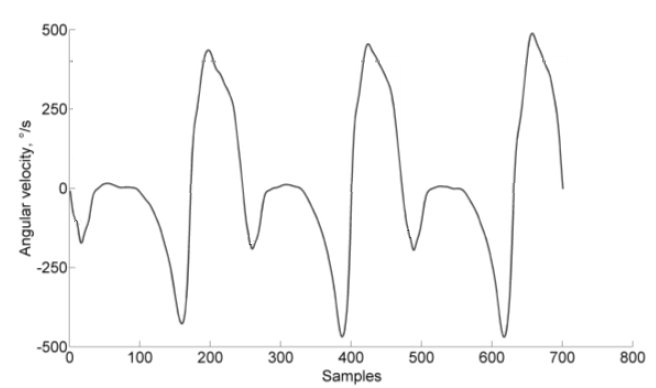
\includegraphics[width=1\textwidth]{imgs/patternGyro.jpg}
	\caption{Grafico del segnale di un giroscopio posizionato sul piede}
	\label{fig:gyroPattern}
\end{figure}

Il grafico del segnale del giroscopio posizionato sul piede ha una struttura abbastanza definita e ripetitiva (vedi grafico \ref{fig:gyroPattern}). Nel grafico, l'ascissa rappresenta i campioni e l'ordinata la velocit� angolare in gradi al secondo ($�/s$). La forma del grafico pu� essere descritta a grandi linee come un picco negativo seguito da un tratto quasi orizzontale ed un secondo picco negativo ed uno positivo. Tale sequenza rappresenta un passo completo e si ripete quasi identica a se stessa durante la camminata.


\begin{table}%
\centering
\begin{tabular}{|c|cc|}
\hline
\textbf{Stato} & \textbf{inizio} & \textbf{fine} \\
%\hline
\hline
$S_1$ & $t_{HS}$ & $t_{FF}$\\
%\hline
$S_2$ & $t_{FF}$ & $t_{HO}$\\
%\hline
$S_3$ & $t_{HO}$ & $t_{FO}$\\
%\hline
$S_4$ & $t_{FO}$ & $t_{HS}$\\
\hline	 
\end{tabular}
\caption{Le quattro fasi della deambulazione e gli eventi (tempo iniziale e finale) che li definiscono.}
\label{tab:4_fasi_deambulazione}
\end{table}
Per semplicit� si pu� indicare uno stato $S_i$ con l'evento da cui ha inizio, ad esempio con lo stato $HS$ indico lo stato $S_1$.

Gli eventi ($t_{HS}$, $t_{FF}$, $t_{HO}$, $t_{FO}$ ) sono determinati mediante soglie, sulla velocit� angolare $\omega_k$, ricavate da studi pregressi \cite{walking_features_from_inertials} come mostra la Tabella \ref{tab:regole_threshold_eventi}, dove $\widetilde{\omega_k}$ � il valore non filtrato del giroscopio.

\begin{table}%
\centering
\begin{tabular}{|c|l p{5cm}|}
\hline
\textbf{Evento} & \multicolumn{2}{c|} {\textbf{regola}}\\
%\hline
\hline
$t_{HS}$ & $ \omega_k \leq 0 $ e $ min_1 \leq  \omega_k$ & $\displaystyle\max_{\forall k}|\widetilde{\omega_k} - \omega_k|$\\
%\hline
$t_{FF}$ & $|\omega_k|\geq  ??$�/sec&\\
%\hline
$t_{HO}$ & $|\omega_k|\geq  50$�/sec &\\
%\hline
$t_{FO}$ & $\omega_k = 0$ & se $\omega$ da negativo � diventato positivo e cresce fino al suo massimo.\\
\hline	 
\end{tabular}
\caption{Regole mediante le quali vengono ricavati gli eventi che delimitano le 4 fasi del cammino.}
\label{tab:regole_threshold_eventi}
\end{table}

Si assume che i segnali del giroscopio siano modellati mediante una HMM:
 \begin{equation}
	Deamb\_HMM = <N, M, \mathbf{A}, \mathbf{B}, \pi>
\label{eq:deamb_hmm}
\end{equation}
dove:
 \begin{enumerate}
	\item $N = 4$ � la cardinalit� dell'insieme degli stati $S = \{HS, FF, HO, FO\}$,
	\item $M = |V|$ � la cardinalit� dell'insieme finito dei valori di osservazione $\omega (^\circ/sec)$ del giroscopio,
	\item $\mathbf{A}$ � la matrice di transizione (vedi appendice \ref{cap:hmm}),
	\item $\mathbf{B}$ � la matrice di probabilit� di emissione delle osservazioni $\omega$ per ciascuno stato. Ad ogni stato � stata associata una funzione di densit� di probabilit� gaussiana univariata.
	\item $\pi$ � il vettore di probabilit� a priori.
\end{enumerate}

A questo punto sono state addestrate le HMM. 
Come prima operazione, � stato etichettato un sottoinsieme dei dati: ad una sequenza $\Omega$ di dati � stato  associato un vettore $Y$ di etichette. Questo � stato fatto con l'uso di un sistema stereofotogrammetrico (sistema di telecamere Vicon).

%Grazie a un analisi di tipo stereofotogrammetrico (sistema di telecamere Vicon (vedi \TODO{Pappas}) sono stati etichettati i dati acquisiti. 

% addestramento HMM 

Dato che nella deambulazione normale le uniche transizioni tra stati sono quelle tra stati contigui o quelle che riportano nello stesso stato, il modello migliore il tipo di HMM scelto � il modello left-right (vedi appendice \ref{sec:tipi_hmm}). Ci� significa che la matrice di transizione gode della propriet� di avere transizioni solo verso stati successivi (da qui il nome "da sinistra - a destra"):
\begin{equation}
	a_{ij} > 0 \quad \text{sse} \quad j=i \quad \text{oppure}\quad j=i+1 \quad \text{oppure} \quad(i = N \quad\text{e}\quad j = 1)
\label{eq:}
\end{equation}
Una volta deciso il tipo di HMM da adottare, si devono stimare i parametri del modello.
La stima (dei parametri del modello) della massima verosimiglianza (Maximum Likelihood Estimation - MLE) $\ell(\Omega, Deamb\_HMM )$ non � un problema convesso dato. Il problema dei massimi locali viene aggirato con un'attenta inizializzazione dei parametri. 

Assumendo che possa avvenire solo una transizione tra stati contigui, in ciascun ciclo di deambulazione possono essere fatte delle stime approssimative dei paramtri della HMM:
\begin{equation}
\begin{split}
\pi_i & = N_i/N_{tot} \\
a_{ij}& = C/N_i \quad \text{dove}\quad j = (i+1)\%Q \\
\mu_i &= \dfrac{1}{N_i} \displaystyle \sum_{t=1}^T{\Omega(t)}\\
\sigma_i &= \sqrt{\dfrac{1}{N_i -1}\displaystyle \sum_{t=1}^T({\Omega(t)-\mu_i})^2}
\end{split}	 
\label{eq:emissionMtx}
\end{equation}
dove $N_i$ � il numero di valori etichettati con l'etichetta $i$-esima nel vettore di etichette $Y$ e $C$ � il numero di cicli di deambulazione nel training set.\\ 
\ERR{VERRI: POCO CHIARO - 
I parametri di emissione ( $\mu$ e $\sigma$) per ciascuno stato $i$ sono stimati calcolando delle medie e deviazioni standard empiriche dagli output osservabili dei quali si conosce lo stato che li ha emessi.\\
}
La validazione � stata fatta con l'approccio leave-one-subject-out cross-validation (LOOCV). 
Il metodo consiste nell'addestrare un modello su P-1 ($P=6$) soggetti e testarne la validit� su 1 soggetto. Ripetendo P volte la procedura per ciascuno dei soggetti alla fine i risultati vengono combinati.\TODO{spiegare come pi� in dettaglio}


Tutta la prima fase della creazione addestramento e validation incrociata del modello � stata fatta off-line, mediante un Mathworks MATLAB (R2008a) ed l'HMM toolbox \cite{HMM_toolbox}. 
Nella fase di test, viene usato l'algoritmo di decodifica di Viterbi \ref{alg:viterbi} sui dati del giroscopio, per trovare la sequenza di stati che con maggior verosimiglianza ha prodotto le osservazioni (sequenze di valori del giroscopio).
Il modello left-right pu� portare a considerare cicli di deambulazione aggiuntivi (insertions), o meno di quelli effettivi (deletions). Il problema delle inserzioni viene risolto mediante l'applicazione di un'euristica: per i presupposti del tipo di deambulazione considerata (velocit� e pendenza del terreno).\\

I parametri del modello stimati da una delle esecuzioni della validazione incrociata � il seguente:
Dati:  HMM



\begin{table}%
\centering
\begin{tabular}{|c|c c c c|}
\hline
\textbf{A} &\textsc{HS} & \textsc{FF} & \textsc{HO} & \textsc{TO}\\
%\hline
\hline
\textsc{HS} & $0.985$ & $0.015$ & $0.0$ & $0.0$\\
%\hline
\textsc{FF} & $0.0$ & $0.998$ & $0.002$ & $0.0$\\
%\hline
\textsc{HO} & $0.0$ & $0.0$ & $0.991$ & $0.009$\\
%\hline
\textsc{FO} & $0.007$ & $0.0$ & $0.0$ & $0.993$\\
\hline	 
\end{tabular}
\caption{Matrice di Transizione}
\label{tab:matrice_transizione}
\end{table}


\begin{table}%
\centering
\begin{tabular}{|c|c c|}
\hline
\textbf{B} &\textsc{$\mu$[�/sec]} & \textsc{$\sigma ^2$[�/sec]}\\
%\hline
\hline
\textsc{HS} & $-52.2$ & $12711.8$\\
%\hline
\textsc{FF} & $-11.8$ & $898.7$\\
%\hline
\textsc{HO} & $-180.1$ & $35806.8$\\
%\hline
\textsc{FO} & $233$ & $14980.3$\\
\hline	 
\end{tabular}
\caption{Matrice di Emissione}
\label{tab:matrice_emissione}
\end{table}


\begin{table}%
\centering
\begin{tabular}{|p{.7cm}|p{2.8cm}|}
\hline
 &\textsc{$\pi$} \\
%\hline
\hline
\textsc{HS} & $0.180$ \\  
%\hline
\textsc{FF} & $0.278$ \\
%\hline
\textsc{HO} & $0.279$ \\
%\hline
\textsc{FO} & $0.264$\\
\hline	 
\end{tabular}
\caption{Distribuzione di probabilit� iniziale}
\label{tab:prior}
\end{table}
Le seguenti sono un esempio di osservazioni: 12400 dati Giroscopio
\begin{table}%
\centering
\begin{tabular}{|c|c|}
\hline
 time&\textsc{$O$} \\
%\hline
\hline
\textsc{1} & $0.37694$\\  
\textsc{2} & $0.37694$\\
\textsc{3} & $0.37694$\\
\textsc{4} & $0.37694$\\
\textsc{5} & $-1.9058$\\
\vdots & \vdots\\
\textsc{24800} & $-16.831$\\
\hline	 
\end{tabular}
\caption{Osservazioni Giroscopio: velocit� angolari}
\label{tab:osservazioni}
\end{table}

%I risultati ottenuti hanno un errore che va dal 3.5\% al 4.7\% che sono errori trascurabili se si considera il numero di fattori in gioco.

%\section[Direzione scelta]{Strategia scelta per la risoluzione del problema dell'analisi del cammino}
%\begin{figure}
%	\centering
%		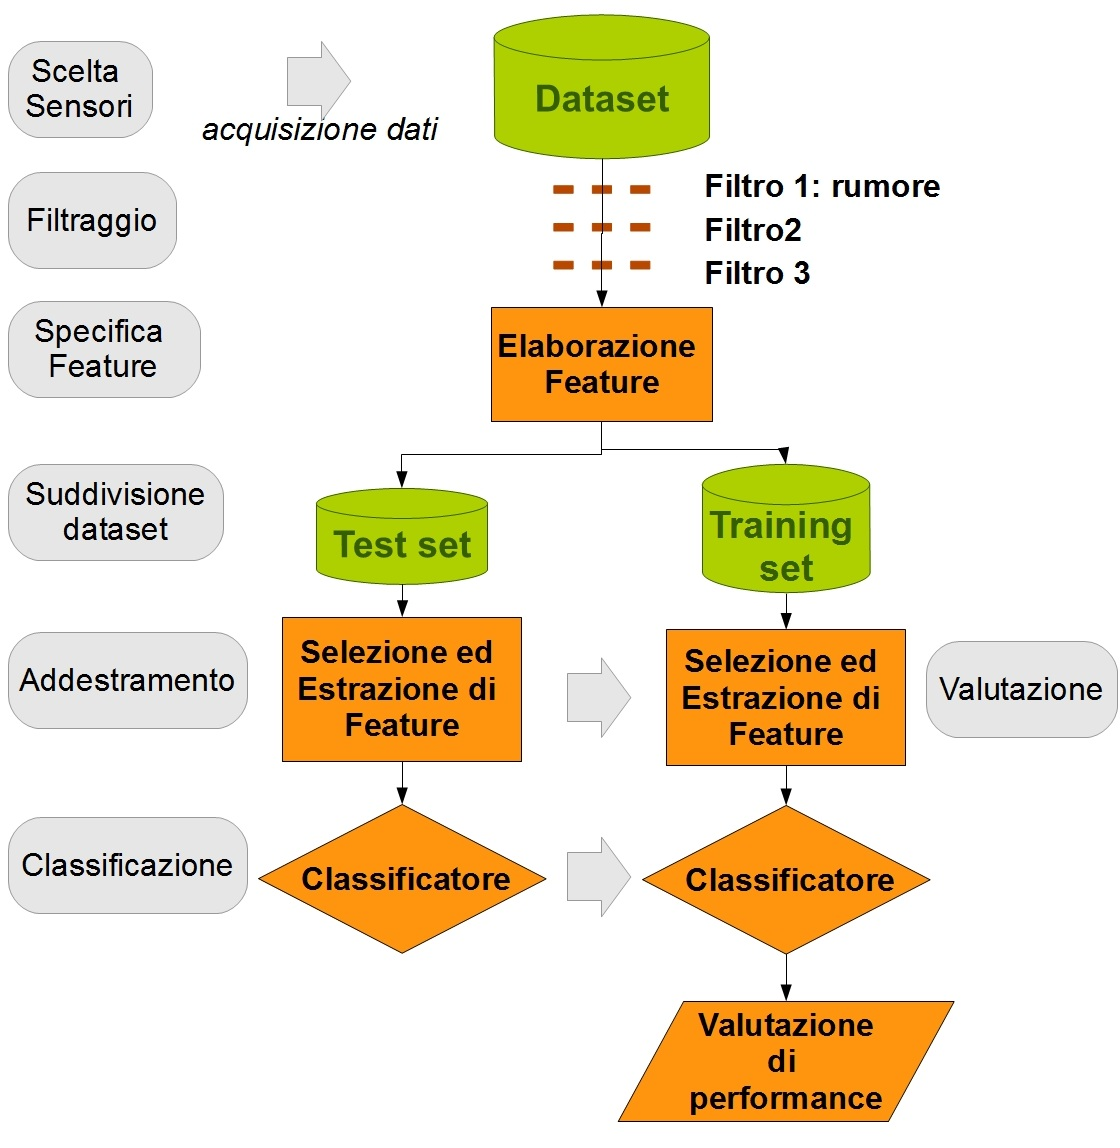
\includegraphics[width=1\textwidth]{imgs/SchemaClassificazioneGenerica.jpg}
%	\caption{Schema concettuale di un sistema di classificazione generico}
%	\label{fig:SchemaClassificazioneGenerica}
%\end{figure}
%\subsection{Selezione dei Sensori}
%\subsection{Acquisizione dei dati}
%\subsection{Specifica delle Feature: valutazione, selezione, estrazione}
%I dati acquisiti devono essere elaborati prima di essere classificati. La classificazione viene fatta su delle rappresentazioni dei dati come variabili di feature (attributi). La scelta dei feature viene fatta caso per caso. 
%La valutazione di feature, avviene spesso in finestre di dimensione fissa che vengono chiamate dataframe. \\
%
%Le feature devono essere selezionate per un triplice motivo: migliorare la performance della classificazione, in modo pi� rapido (perch� diminuisce il numero di variabili della computazione)e fornire una comprensione migliore del processo sottostante alla generazione dei dati in considerazione. 
%Guyon et al.\cite{intro_variable_feature_selection} nel loro articolo danno un algoritmo euristico per una buona selezione di feature:
%
%\begin{enumerate}
%	\item \textbf{Conosci il dominio del problema?} Se si, costruisci un insieme migliore di feature ad-hoc.
%	\item \textbf{Le tue feature sono proporzionate?} Se no normalizzale.
%	\item \textbf{Sospetti un'interdipendenza di feature?} Se si, espandi il tuo insieme di feature, costruende feature congiuntive o prodotti di feature, al massimo delle potenzialit� del tuo computer.
%	\item \textbf{Devi potare le variabili di input (per motivi di velocit�, o migliore comprensione dei dati)?} Se no, costruisci delle feature disgiuntive o somme pesate di feature (ad esempio per raggruppamenti (clustering) o fattorizzazioni di matrici)
%\item \textbf{Devi valutare delle feature individualmente (ad esempio per capire il loro impatto sul sistema o perch� sono cos� tanti che devi prima fare un filtraggio?)} Se si, usa un metodo di ranking di variabili, altrimenti fallo lo stesso per avere dei risultai di partenza. 
%\item \textbf{Sospetti che i tuoi dati siano spuri? (Hanno alcuni input senza senso o output con del rumore o con etichette di classi errate)}.Se si, individua gli esempi sbagliati con il ranking del passo precedente come gli esempi con il punteggio pi� alto ed esaminali o eliminali. 
%\item \textbf{Sai cosa provare prima?} Se no, usa un predittore lineare. Usa un metodo di selezione forward, con un un criterio di arresto a sonda (probe). Per confrontare i risultati, in base al ranking, costruisci una sequenza di predictor, che si differenzino solo per la grandezza del sottoinsieme di feature che usano.
%Puoi ridurre le dimensioni dei sottoinsiemi ed avere una performance pari o addirittura migliore? Se si, prova un predictor non-lineare con quel particolare sottoinsieme. 
%\end{enumerate}
%
%\subsection{Valutazione}
%\subsection{Selezione}
%\subsection{Estrazione}
%\subsection{Fase di addestramento}
%\subsection{Selezione ed Estrazione delle Feature}
%\subsection{Classificazione}
%
%\subsection{Fase di valutazione}
%\subsection{Selezione ed Estrazione delle Feature}
%\subsection{Classificazione}
%\subsection{Valutazione di performance}
%
%
%\section{Hardware}
%IMU \footnote{Inertial Measurement Unit}
%\begin{itemize}
%	\item Scheda -- dimensioni--processore, RAM, memoria FLASH
%	\item Bluetooth
%	\item Gyroscope
%\end{itemize}
%\section{software}
%\begin{itemize}
%	\item sistema operativo IMU
%	\item protocollo di comunicazione Mailbox
%	\item Ambiente Android 
%	\item Algoritmi di Machine Learning 
%\end{itemize}



\chapter{Applicativo Android}
%\myChapter{Applicativo Android}
%%%%%%%%%%%%%%%%%%%%%%%%%%%%%%%%%%%%%%%%%%%%%%%%%%%%%%%%%%%%%%%%%%%%%%%%%%%%%%%%%%%%%%%%%%%%%%%%%%%%%%%%%%%%%%%%%%%%%%%%%%%%%%%%%%%%%%%%%%%%%%%%%%%%%%%%%%%%%%%%%%%%%%%%%%%%%%%%%%%%%%%%%%%%%%%%%%%%%%%%%%%%%%%%%%%%%%%%%%%%%%%%%%%%%%%%%%%%%%%%%%
\section{Introduzione}%descrivere cosa fa a grandi linee %%%%%%%%%%%%%%%%%%%%%%%%%                           INTRODUZIONE

La seconda parte del lavoro, � relativa all'implementazione di algoritmi di segmentazione online su uno Smartphone Android. L'applicativo in oggetto,  sulla base di un modello HMM addestrato offline (vedi sezione \ref{sec:creazione_addestramento_modello}), impiega una versione dell'algoritmo di Viterbi \cite{short_time_viterbi_online_hmm_deconding} per elaborare a run-time i dati giroscopici acquisiti dalla IMU (e trasferiti via Bluetooth), effettuando la segmentazione e consentendo output di tipo grafico (colorando in modo differente la traccia del segnale giroscopico in funzione della fase del cammino), e di data logging. 

%%%%%%%%%%%%%%%%%%%%%%%%%%%%%%%%%%%%%%%%%%%%%%%%%%%%%%%%%%%%%%%%%%%%%%%%%%%%%%%%%%%%%%%%%%%%%%%%%%%%%%%%%%%%%%%%%%%%%%%%%%%%%%%%%%%%%%%%%%%%%%%%%%%%%%%%%%%%%%%%%%%%%%%%%%%%%%%%%%%%%%%%%%%%%%%%%%%%%%%%%%%%%%%%%%%%%%%%%%%%%%%%%%%%%%%%%%%%%%%%%%
\section{Metodologia di programmazione usata: Agile}%agile %%%%%%%%%%%%%%%%%         METODOLOGIA DI PROGRAMMAZIONE
\label{sec:agile}
Per l'implementazione dell'algoritmo di Viterbi e le funzioni utilizzate nella fase di analisi del segnale, � stata utilizzata una tecnica nota come Agile Programming. Una tecnica che permette lo sviluppo di programmi in cicli di lavoro iterativi ed incrementali in termini di funzionalit�. 
\begin{enumerate}
	\item Scrittura di uno Unit Test\footnote{Per Unit si intende la pi� piccola parte di un programma che pu� essere testata, nei linguaggi orientati ad oggetti un metodo costituisce un'unit�. Per Unit testing si intende la verifica del funzionamento di singole Unit. }. Lo Unit Test istanza l'oggetto dalla classe da testare, ed invoca il metodo con valori per i quali � noto il comportamento (teorico) del metodo da testare.\\
Il test viene eseguito, per la prima volta, prima di aver implementato il metodo da testare, ed ovviamente fallisce\footnote{Eclipe IDE \tm utilizza il framework JUnit che semplifica la gestione degli Unit Test.}. Il passo successivo � di implementare il minimo indispensabile per far funzionare il test. Se il test viene superato dal codice scritto, viene scritto un altro test, ed un altro pezzo di codice, iterando la procedura finch� non si ha tutto il programma desiderato.\\ 
A titolo di esempio di seguito verr� illustrato lo sviluppo della classe che gestisce le operazioni di tipo statistico:
\begin{lstlisting}[language=java, style=eclipse, caption=Sviluppo di una classe mediante la tecnica di programmazione Agile, label=code:agile1]
// la classe da costruire 
public class StatisticsOperations{...}
// l'insieme di test
public class StatisticsOperationsTest extends TestCase {...}
\end{lstlisting}


Le operazioni necessarie per lavorare sulle HMM erano: 
\begin{itemize}
	\item verificare la validit� di valori di probabilit�
	\item verificare la completezza di un insieme di alternative probabilistiche
	\item calcolare la Probabilit� di un dato assumendo quanto estratto da una distribuzione Normale ($ \mathcal{N}(x,\mu, \sigma)$) con media $\mu$ e varianza $\sigma^2$ note.
\end{itemize}
Creazione delle le firme dei metodi
\begin{lstlisting}[language=java, style=eclipse, caption=Firme dei metodi da implementare, label=code:agile2]
public class StatisticsOperations{	
	public static boolean areCompleteProbabilisticAlternatives(ArrayList<Object> alternatives) {...}
	public static boolean isValidProbabilityValue(double value) {...}
	public static double gaussian(double x, double mu, double sigma_square) {...}
}
\end{lstlisting}
\item Creazione di un test vuoto (destinato a fallire).
\item Implementazione dei test per cinque casi rappresentativi dei degli intervalli esterni ed interni a quello di riferimento (0,1).

\begin{lstlisting}[language=java, style=eclipse, caption=Casi di test di contorno, label=code:agile3]
public class StatisticsOperationsTest extends TestCase {
	... // metodi setUp e tearDown che per ora non uso
	
	public void testIsMinusOneACorrectProbabilityValue() {
		boolean expected = false;
		boolean actual = StatisticsOperations.isValidProbabilityValue(-1);
		assertEquals(expected, actual);
	}
	public void testIsZeroACorrectProbabilityValue() {
		boolean expected = true;
		boolean actual = StatisticsOperations.isValidProbabilityValue(0);
		assertEquals(expected, actual);
	}
	public void testIsPointFiveACorrectProbabilityValue() {
		boolean expected = true;
		boolean actual = StatisticsOperations.isValidProbabilityValue(.5);
		assertEquals(expected, actual);
	}
	
	public void testIsOneACorrectProbabilityValue() {
		boolean expected = true;
		boolean actual = StatisticsOperations.isValidProbabilityValue(1);
		assertEquals(expected, actual);
	}
	
	public void testIsTwoACorrectProbabilityValue() {
		boolean expected = false;
		boolean actual = StatisticsOperations.isValidProbabilityValue(2);
		assertEquals(expected, actual);
	}
	
	public void testIsRandNumACorrectProbabilityValue() {
		boolean expected = false;
		double randomProbabilityValue = Math.random();
		if (randomProbabilityValue >= 0 && randomProbabilityValue <= 1){
			expected = true;
		}
		boolean actual = StatisticsOperations.isValidProbabilityValue(randomProbabilityValue);
		assertEquals(expected, actual);
	}

}
\end{lstlisting}

\item Sviluppo del corpo del metodo che si sta testando. Questa fase (la pi� importante) � notevolmente agevolata dalle precedenti. Il programmatore ha chiare la funzione da implementare e le relative problematiche. 
\begin{lstlisting}[language=java, style=eclipse,caption=Implementazione dei metodi da testare, label=code:agile4]
public class StatisticsOperations{	
	public static boolean areCompleteProbabilisticAlternatives(ArrayList<Object> alternatives) {...}
	public static boolean isValidProbabilityValue(double value) {
		if (value >= 0 && value <= 1)
			return true;
		else
			return false;
}
	public static double gaussian(double x, double mu, double sigma_square) {...}
}
\end{lstlisting}
\end{enumerate}
La esecuzione del test sul metodo riscritto porta ad uno dei seguenti esiti:
\begin{enumerate}
	\item superamento di tutti i test, quindi lo sviluppo del metodo � completato,
	\item fallimento di almeno un test, il metodo deve essere corretto ed i test devono essere nuovamente eseguiti.
\end{enumerate}

%%%%%%%%%%%%%%%%%%%%%%%%%%%%%%%%%%%%%%%%%%%%%%%%%%%%%%%%%%%%%%%%%%%%%%%%%%%%%%%%%%%%%%%%%%%%%%%%%%%%%%%%%%%%%%%%%%%%%%%%%%%%%%%%%%%%%%%%%%%%%%%%%%%%%%%%%%%%%%%%%%%%%%%%%%%%%%%%%%%%%%%%%%%%%%%%%%%%%%%%%%%%%%%%%%%%%%%%%%%%%%%%%%%%%%%%%%%%%%%%%%
\section{Organizzazione del programma}%%%%%%%%%%%%%%%%%%%%%%%%%%%%%%%%%%%%%%%%%%%%%%%              ORGANIZZAZIONE DEL CODICE
\subsection{Android Manifest} AndroidManifest.xml (vedi Appendice \ref{sec:android_app_structure}) � il file che viene usato come punto di partenza e di riferimento dal compilatore Dalvik (vedi Appendice \ref{sec:dalvik}). 


\begin{lstlisting}[language=XML, style=xmlandroid, caption=AndroidManifest testata, label=code:manifest_permissions]
<?xml version="1.0" encoding="utf-8"?>
<manifest xmlns:android="http://schemas.android.com/apk/res/android"
	package="imu.Interface" android:versCode="1" android:versName="1.0">
\end{lstlisting}
Il nome del Java package, serve come identificativo unico per l'applicativo.

\begin{lstlisting}[language=XML, style=xmlandroid,caption=AndroidManifest permessi,label=code:manifest_permissions, firstnumber=3]
	<uses-permission android:name="android.permission.BLUETOOTH" />
	<uses-permission android:name="android.permission.BLUETOOTH_ADMIN" />
	<uses-permission android:name="android.permission.WRITE_EXTERNAL_STORAGE" />
	<uses-sdk android:minSdkVersion="8" />
	...
\end{lstlisting}

%%%%%%%%%%%%%%%%%%%%%%%%%%%%%%%%%%%%%%%%%%%%%%%%%%%%%%%%%%%%%%%%%%%%%%%%%%%%%%%%%%%%%%%
%%%%%%%%%%%%%%%%%%%%%%%%%%%%%%%%%%%%% modifica 24 nov %%%%%%%%%%%%%%%%%%%%%%%%%%%%%%%%%
%%%%%%%%%%%%%%%%%%%%%%%%%%%%%%%%%%%%%%%%%%%%%%%%%%%%%%%%%%%%%%%%%%%%%%%%%%%%%%%%%%%%%%%
Dato che il nucleo di Android-OS � Linux (vedi Appendice \ref{app:android}) usa una politica di {Access Control}\footnote{Accesso controllato dell'utente di un filesystem o di un servizio} molto simile. Tutti i servizi che non sono forniti dal contesto di questo particolare applicativo, quindi i servizi che fornisce l'applicativo stesso, e quelli forniti dal sistema operativo per tutti gli applicativi, possono essere utilizzati solo se l'utente da il permesso di utilizzarli. Per questo motivo l'applicativo deve elencare tutte le richieste di permessi di cui necessita. L'elenco deve essere fatto nella porzione iniziale dell'\verb|AndroidManifest|
 Dichiarazione dei permessi che l'applicativo deve avere dall'utente per accedere ad alcune parti dell'API\footnote{ Application Programming Interface: interfaccia ad un codice che viene messo a disposizione come servizio in modo che terzi possano usarlo per sviluppare altro software, avvolte anche in altri linguaggi.
 In dettaglio una API nei linguaggi orientati ad oggetti, sono concepiti come l'insieme di tutti i metodi pubblici che le classi pubbliche offrono.} di Android e per interagire con altri applicativi.
 La riga 4 chiede il permesso di fare la discovery (ricerca) di dispositivi e di associarsi  a dispositivi trovati, la riga precedente invece il permesso di connettersi a dispositivi associati \footnote{L'associazione � la prima connessione, nella quale vi � una forma di identificazione e associazione dei due dispositivi. Per connessione invece si intendono le connessioni successive alla prima, in cui un dispositivo conosce gi� l'altro e, pi� rapidamente, possono iniziare una conversazione.}. L'ultimo permesso serve per poter scrivere su un dispositivo d'immagazzinamento esterno, questo ci serve per poter salvare ad esempio l'output dell

 
\begin{lstlisting}[language=XML, style=xmlandroid,caption=AndroidManifest dichiarazione dell'attivit� principale, label=code:manifest_application, firstnumber=8]
	<application android:icon="@drawable/spinningtop02"
		android:label="@string/app_nameicon" 
		android:name="imu.objects.MailBoxes">
\end{lstlisting}
Vengono dichiarati il nome dell'applicativo, l'icona, ed un'etichetta. In questo punto si dichiara anche il nome dell'oggetto che pu� essere visibile a livello globale di applicativo. Infatti l'oggetto \verb|MailBoxes| che � un vettore di \verb|MailBox| (vedi \ref{sec:mailbox}) che sono a loro volta utilizzati per lo scambio di dati tra thread.

\begin{lstlisting}[language=XML, style=xmlandroid,caption=AndroidManifes elenco di tutte le attivit� ,label=code:manifest_activities, firstnumber=11]		
		<activity android:name=".IMUinterface" android:configChanges="orientation">
			<intent-filter>
				<action android:name="android.intent.action.MAIN" />
				<category android:name="android.intent.category.LAUNCHER" />
			</intent-filter>
		</activity>
		<activity android:name=".Saveactivity" android:label="@string/save_name" />
		<activity android:name=".SensSetupactivity" android:label="@string/sens_name" />
		<activity android:name=".Provaactivity" android:label="@string/prova_name" />
		<activity android:name=".EmbeddedSensDataPlottingvActivity"
			android:label="@string/prova_name" android:configChanges="orientation"
			android:theme="@android:style/Theme.NoTitleBar.Fullscreen" />
		<activity android:name=".TemporalDataPlottingvActivity"
			android:configChanges="orientation" android:theme="@android:style/Theme.NoTitleBar.Fullscreen" />
\end{lstlisting}	
Sezione di \verb|AndroidManifest| in cui si elencano i componenti fondamentali (vedi Appendice \ref{sec:android_main_components}) utilizzati nell'applicativo.
Il nostro applicativo, che ha una struttura molto semplice, ed utilizza solo \verb|Activity| ed \verb|Intent|. 
Il l'Activity principale (Main Activity) � \verb|IMUInterface|.\\ 
La dichiarazione di una Activity � composta da un nome e da una classe Java.
Inoltre sono dichiarate altre impostazioni iniziali: se sono gestiti o meno i 2 orientamenti dello schermo, se lo schermo deve essere visualizzato senza la barra dei titoli in testa allo schermo.

\subsection{Codice sorgente}
Tutto il codice sorgente (Java) deve essere contenuto nella cartella \emph{src} del progetto. 
Abbiamo strutturato il codice in 5 package (cartelle di Java):
\begin{itemize}
	\item \textbf{activities}: le Activity, corrispondono indicativamente ciascuna ad una schermata sullo Smartphone,
	\item \textbf{objects} : dati, modelli o contenitori su cui fare operazioni,
	\item \textbf{services}: operazioni fondamentali dell'applicativo, che qui coincidono agli algoritmi che si applicano alla HMM. 
	\item \textbf{tests}: test prodotti dall'utilizzo della metodologia Agile (vedi \ref{sec:agile}),
	\item \textbf{util}: operazioni di supporto al resto del codice. 
\end{itemize} 

\subsection{Risorse}
Le risorse sono costituite da tutti i file che fanno parte dell'applicativo, ma non sono codice sorgente (vedi Appendice \ref{sec:android_app_structure}) vale a dire file xml, immagini, testo ecc. La sezione pi� importante delle risorse � la cartella \textbf{layout}. Questa contiene una serie di file xml, che in teoria, per ciascuna Activity dovrebbe essere creato un file xml da mettere nella cartella layout, con lo stesso nome della Activity.
\subsubsection{Layout}
Un file di layout (impaginazione) � un documento xml in cui viene descritta la struttura dell'interfaccia utente di una Activity.
Layout deve essere composto di elementi grafici predefiniti in Android oppure deve essere di tipo \verb|Veiw| o  \verb|ViewGoup|\footnote{Sia la View che la ViewGroup appartengono al package android.view e sono componenti importante dell'interfaccia utente}. Ogni file di layout deve contenere esattamente un elemento radice. Ogni elemento grafico ha un identificativo unico, con cui pu� essere richiamato dal codice sorgente, tramite l'indicizzazione automatica.
Eclipse \tm permette di definire un layout sia in modalit� xml che in modalit� grafica (WYSIWYG\footnote{What You See Is What You Get}). Ad esempio il layout della activity principale (ImuInterface) � il seguente 
\begin{lstlisting}[language=XML, style=xmlandroid,caption=LinearLayout:impaginazione  della schermata principale,label=code:mainActivity_layout_linear]
<?xml version="1.0" encoding="utf-8"?>
<LinearLayout xmlns:android="http://schemas.android.com/apk/res/android"
	android:orientation="vertical" android:layout_width="fill_parent"
	android:background="#111111" android:layout_height="fill_parent">
\end{lstlisting}
Un \verb|LinearLayout| � un tipo di layout che pu� contenere altri layout, in sostanza serve ad organizzare oggetti. Sono impostate alcune delle propriet� (orientamento, larghezza ecc) dell'oggetto.  
\begin{lstlisting}[language=XML, style=xmlandroid,caption=TextView: oggetto contenente testo ,label=code:mainActivity_layout_text, firstnumber=5]
	<TextView android:layout_height="wrap_content" 
		android:text="@string/ImuActivity_title" android:textStyle="bold"
		android:id="@+id/AppName" android:layout_width="320dip">
	</TextView>
\end{lstlisting}	
Questo � un oggetto che contiene testo non modificabile dall'utente. Qui viene visualizzato il titolo della schermata, contenuto nella variabile di stringa \verb|"@string/ImuActivity_title"|.

\begin{lstlisting}[language=XML, style=xmlandroid,caption=EditText:oggetto contenente campi di testo modificabili,label=code:mainActivity_layout_text, firstnumber=9]
	<EditText android:id="@+id/editText1" 
		android:layout_height="wrap_content" 
		android:layout_width="match_parent">
	</EditText>
	<EditText android:id="@+id/editText2"
		android:layout_height="wrap_content" 
		android:layout_width="match_parent">
	</EditText>
	....
\end{lstlisting}	
Vi sono subito sotto il titolo della schermata, quattro campi di testo (di cui sono riportate solo 2 a titolo illustrativo). 


\begin{lstlisting}[language=XML, style=xmlandroid,caption=Esempio di LinearLayout contenente un Button,label=code:mainActivity_layout_text, firstnumber=25]
	<LinearLayout android:background="#111111"
		android:layout_height="fill_parent" 
		android:layout_weight="1"
		android:layout_width="fill_parent" 
		android:orientation="horizontal">
		...
		<Button android:id="@+id/button2" android:layout_height="wrap_content"
			android:text="Start" android:gravity="center_vertical|center_horizontal"
			android:layout_width="55dip">
		</Button>
		...
	</LinearLayout>
	...
\end{lstlisting}

La parte seguente della schermata, percorrendola dall'alto verso il basso, � un altro \verb|LineraLayout| contenente altri campi di testo e bottoni.\\
La schermata risultante dal layout � quella dell'immagine \ref{fig:main_activity}.
\begin{figure}
	\centering
		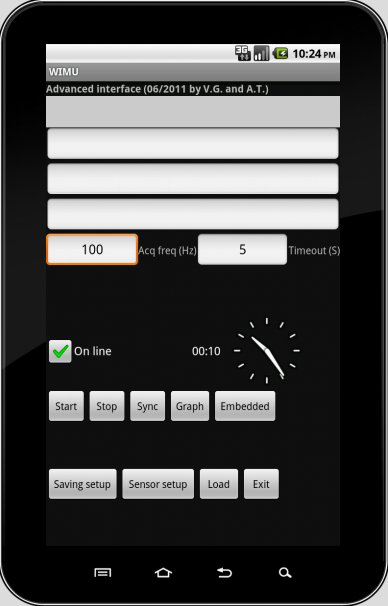
\includegraphics[width=.7\textwidth]{imgs/MenuActivity.jpg}
	\caption{Schermata della Activity iniziale dell'applicativo}
	\label{fig:main_activity}
\end{figure}
\subsubsection{File grafici}
I file grafici sono distribuiti su tre cartelle \textbf{drawable-hdpi}, \textbf{drawable-ldpi},\textbf{drawable-mdpi} in cui salvare formati a definizioni diverse delle stesse immagini per diversi dispositivi. 
\subsubsection{Valori}
Il file pi� importante in questa cartella � \verb|strings.xml| in cui vengono salvate tutte le stringhe da visualizzare sulle varie schermate. L'utilit� maggiore di mantenere le stringhe in un file unico, � l'internazionalizzazione dell'applicativo. Con il tipo di mercato mondiale che hanno gli applicativi Android, avere il testo tradotto in pi� lingue � necessario.
\subsubsection{Altri File}
Qualunque tipi di file, che non sia compatibile con quelli menzionati precedentemente, vanno nella cartella \verb|raw|. Ad esempio, in fase di sviluppo, per testare l'algoritmo di Viterbi, abbiamo usato un file contenente dati di un giroscopio, acquisito nella fase precedente del lavoro. 
\subsection{Librerie}
Le librerie usate sono quelle di Android 2.2 (vedi Appendice \ref{sec:lib_Android}).
%%%%%%%%%%%%%%%%%%%%%%%%%%%%%%%%%%%%%%%%%%%%%%%%%%%%%%%%%%%%%%%%%%%%%%%%%%%%%%%%%%%%%%%%%%%%%%%%%%%%%%%%%%%%%%%%%%%%%%%%%%%%%%%%%%%%%%%%%%%%%%%%%%%%%%%%%%%%%%%%%%%%%%%%%%%%%%%%%%%%%%%%%%%%%%%%%%%%%%%%%%%%%%%%%%%%%%%%%%%%%%%%%%%%%%%%%%%%%%%%%%
\section{Funzionamento}%%%%%%%%%%%%%%%%%%%%%%%%%%%%%%%%%%%%%%%%%%%%%%%%%%%%%%%%%%%                         FUNZIONAMENTO 
\subsection{Interfaccia}
La linea guida per lo sviluppo della UI (Interfaccia Utente) � stata quella della massima ergonomicit�, in linea con la filosofia di sviluppo di interfacce utente di Android. \\
La navigazione tra le schermate dell'applicativo � guidata da widget che sono oggetti grafici della UI di un programma, che hanno lo scopo di facilitare all'utente l'interazione con il programma. \\
All'avvio del programma, viene visualizzato sullo schermo del dispositivo, un menu dal quale � possibile 

\begin{figure}
	\centering
		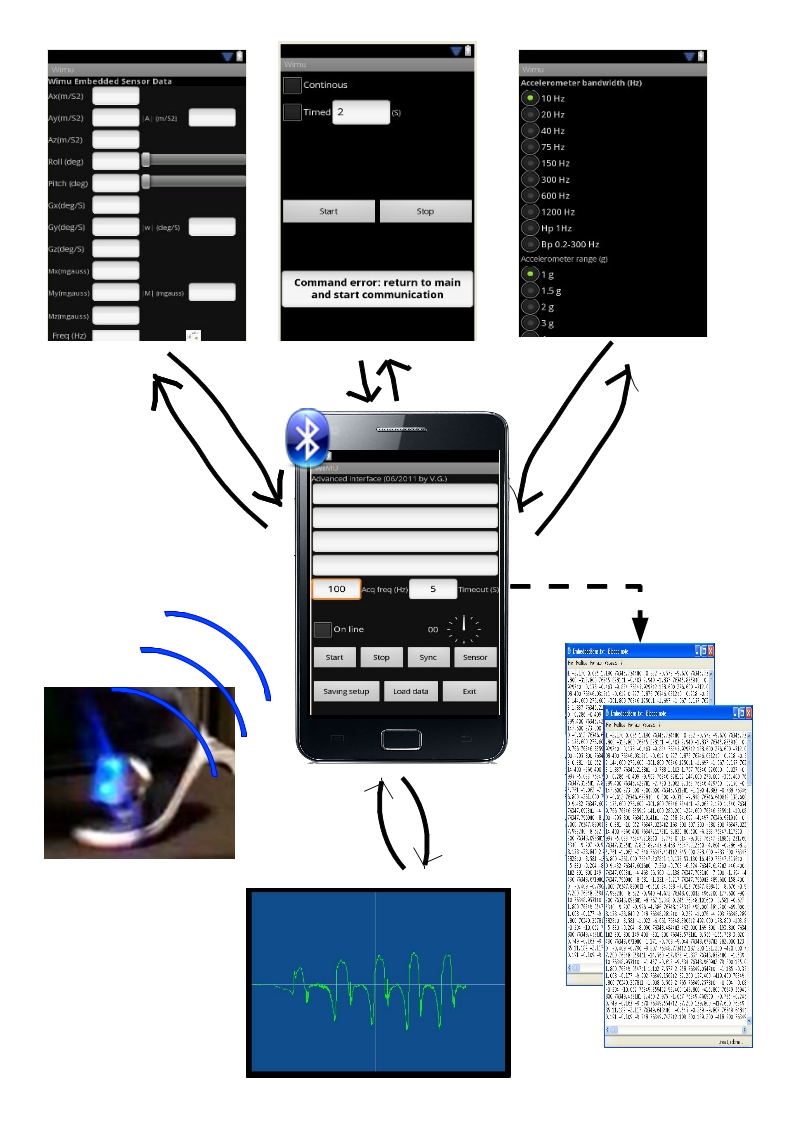
\includegraphics[width=1\textwidth]{imgs/interfacciaApplicativo.jpg}
	\caption{Collegamento fra le schermate dell'applicativo}
	\label{fig:app_UI}
\end{figure}

\subsection{Comunicazione Bluetooth}
\label{sec:bluetooth_adapter}
\verb|BluetoothAdapter|
Rappresenta l'adattatore Bluetooth del dispositivo locale e permette di fare le operazioni pi� importanti sullo stesso:
\begin{itemize}
	\item Ricerca (discovery) di dispositivi, 
	\item Query su una lista di dispositivi connessi,
	\item istanziazione di un dispositivo Bluetooth (\verb|BluetoothDevice|) usando un indirizzo MAC noto,
	\item creazione di una server-socket (\verb|BluetoothServerSocket|) per accettare richieste di connessione da altri dispositivi Bluetooth.
\end{itemize}
\subsection{Gestione della connessione}
\verb|ConnectThread| � un \verb|\Runnable| che gestisce le connessioni mediante thread. Dati un dispositivo \verb|BluetoothDevice|, un adattatore \verb|BluetoothAdapter| ed il numero identificativo del dispositivo, 
se questo non � connesso, viene creata una socket RFComm con l'UUID pronta per una comunicazione. All'avvio del thread (con il metodo \verb|run()|) avviene la connessione. Il thread lancia a sua volta un thread al quale delega la gestione delle socket create (\verb|manageConnectedSocket|). Quest'ultimo invia un segnale di inizio acquisizione dati sui canali creati e li acquisisce se disponibili.

\subsection{Gestione Thread}
Il sistema operativo Android � multithread. Un applicativo che risponda rapidamente alle richieste dell'utente deve necessariamente smistare i compiti a pi� thread, dando la precedenza ai thread di risposta all'utente. Il pi� importante di questi � lo UI Thread (User Interface Thread). Una regola di base della programmazione di applicativi Android �, nella creazione di un'activity, che si deve assolutamente evitare di sovraccaricare, o ancora peggio, eseguire istruzioni potenzialmente bloccanti all'interno dello UI Thread. La prassi per la gestione di operazioni con un comportamento imprevedibile dal punto di vista temporale, come ad esempio le operazioni di rete o di lettura e scrittura di file, � di incaricare altri thread che possano, se necessario, essere eseguiti in background, o fermati se necessario.\\
Abbiamo ritenuto utile avere un protocollo di comunicazione fra thread mediante una struttura che abbiamo chiamato "mailbox", in cui $n$ thread possano inserire e consumare dati.\\
\subsubsection{MailBox}
\label{sec:mailbox}
L'oggetto \verb|MailBox| � un buffer di tipo generico, a cui si pu� accedere per ora solo mediante un inserimento ed un prelievo sincronizzati, ma ci� potrebbe essere facilmente esteso a 3 modalit�:
\begin{enumerate}
	\item \textbf{Sincronizzata}: l'inserimento e prelievo di dati dalla mailbox � bloccante, un thread inserisce un dato se c'� spazio nel buffer, un altro thread utilizza il dato, se esiste. Ciascuno attende il proprio turno per compiere l'azione. La sincronizzazione viene gestita con un meccanismo di semafori che Java fornisce.
	I metodi di accesso sono:

	
\begin{lstlisting}[language=java, style=eclipse,label=code:mailbox_put_get]
	synchronized public void put(T object)
	synchronized public T get()
\end{lstlisting}


	Un thread alla volta pu� prendere, in mutua esclusione, l'accesso in scrittura al buffer, chiamando per primo il metodo \verb|put| (vedi algoritmo \ref{alg:mailbox_put}). Il valore contenuto nel buffer � sempre visibile a tutti i thread. Questo risultato � stato ottenuto dichiarando la variabile con la parola chiave \verb|volatile|. 
\begin{lstlisting}[language=java, style=eclipse]
	volatile private T buffer = null;
\end{lstlisting}
Normalmente, ci� che avviene al momento in cui un thread prende l'accesso in mutua esclusione ad una variabile, � che si copia nel proprio stack di lavoro la variabile e modifica quella e solo prima di rilasciare la variabile la aggiorna all'esterno. Altri thread che fossero abilitati a vedere la variabile nel momento in cui � in modifica, vedrebbero un valore incongruente con il valore reale della stessa. La parola chiave volatile, impedisce ai thread che la modificano di crearsene una copia, e li vincola a lavorare direttamente sulla variabile\footnote{la parola chiave volatile impedisce un possibile ripristino del valore di una variabile, il che rende potenzialmente pericolosa per la perdita di dati} garantendone la visibilit� in tutti i momenti.\\ 

\begin{lstlisting}[language=java, style=eclipse,label=code:mailbox_put]
synchronized public void put(T object){
	//se il buffer � vuoto
	if (buffer == null){
		//inserisci l'oggetto
		buffer = object;
		//notifica tutti i thread in attesa sul buffer
		this.notifyAll();
	}else{
		try{
			//altrimenti attendi una notifica sul buffer
			this.wait();
			buffer = object;				
		}catch (InterruptedException e) {
			e.printStackTrace();
		}
	}
}
\end{lstlisting}
 

Un thread pu� prelevare il dato immesso da un altro nella mailbox, usando il metodo \verb|get()|(vedi algoritmo \ref{alg:mailbox_get}). Mentre il dato viene prelevato, questo non pu� essere modificato. Appena il thread ha preso il dato, lo elimina dal buffer.

\begin{lstlisting}[language=java, style=eclipse,label=code:mailbox_get]
synchronized public T get(long d){
	T temp = null;
	//il buffer � vuoto
	if(buffer == null){
		try {
			//attendi una notifica sul buffer
			this.wait();
			//salva il contenuto del buffer
			temp = buffer;
			//svuoto il buffer
			buffer = null;
		} catch (InterruptedException e) {
			e.printStackTrace();
		}
	} else {
		temp = buffer;
		buffer = null;			
		//notifica tutti i thread in attesa sul buffer
		this.notifyAll();
	}
	return  temp; }
\end{lstlisting}

Queste due operazioni implicano che devono essere eseguite in ordine, ed alternati ($put(dato_i)$, $get()$, $put(dato_j)$, $get()$ ecc ).

\item \textbf{Temporizzata}: ci� che avviene � molto simile al caso precedete: i thread vengono sincronizzati sul buffer. La differenza � che attendono solo una predeterminata quantit� di tempo prima di inserire dati nuovi nel buffer. Ci� significa che sovrascrivono qualunque dato non sia stato consumato in tempo.

\item \textbf{Condizionata}: la variante, in questo caso, sta nel superare l'attesa in scrittura nel momento in cui si verifichi una determinata condizione. 

\end{enumerate}


\subsubsection{Test per il protocollo di comunicazione MailBox}

Il primo esperimento riuscito sul protocollo � stato quello di due thread, un produttore ed un consumatore che comunicano tramite una \verb|MailBox|. Il produttore genera una sequenza ordinata di numeri dispari, crea un oggetto \verb|Point| nel seguente modo:
\begin{lstlisting}[language=java, style=eclipse,caption=Creazione di un oggetto Point,label=code:mailbox_experiment]
new Point(x++, Math.sin(x))
\end{verbatim}

L'oggetto cos� creato viene inserito dallo stesso produttore nella MailBox. Il consumatore pu� tentare di prelevare l'oggetto chiamando \verb|get()|. Mandando in stampa su console una sessione di comunicazioni si ha:

\begin{table}%
\centering
\begin{tabular}{l l}
put:& (70913.0, 0.921)\\
get:& (70913.0, 0.921)\\
put:& (70915.0, -0.737)\\
get:& (70915.0, -0.737)\\
put:& (70917.0, -0.307)\\
get:& (70917.0, -0.307)\\
put:& (70919.0, 0.993)\\
get:& (70919.0, 0.993)\\
put:& (70921.0, -0.519)\\
get:& (70921.0, -0.519)\\
put:& (70923.0, -0.561)\\
get:& (70923.0, -0.561)\\
put:& (70924.0, 0.393)
\end{tabular}
\caption{Sequenza di scritture su console da parte di un thread che crea la coppia (x, sin(x)) e da un altro che consuma il valore usando il protocollo MailBox}
\end{table}
 
Ho reimplementato lo stesso esperimento su Android, con una semplice activity per visualizzare il punto generato dal thead produttore, come il centro di un cerchio.
\begin{figure}
	\centering
		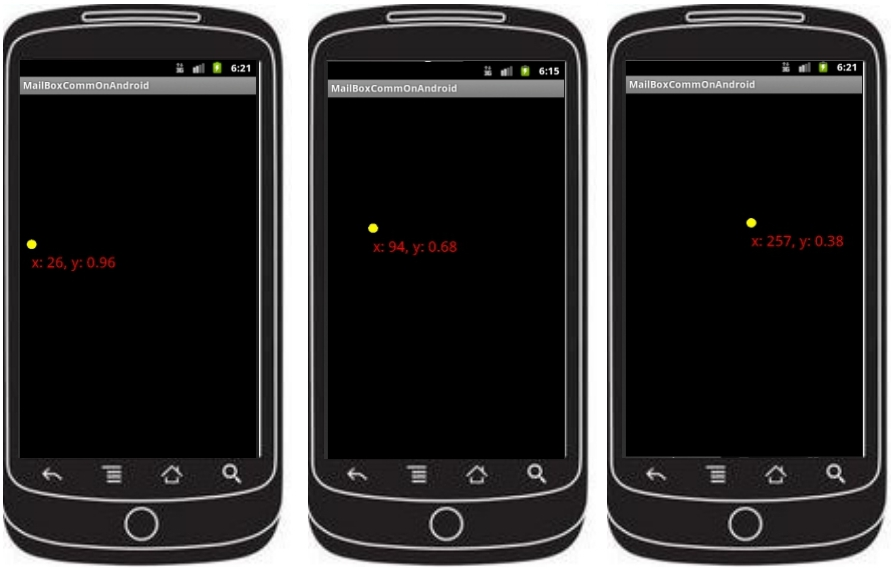
\includegraphics[width=.6\textwidth]{imgs/MailBoxCommTestAndroid.jpg}
	\caption{Prova di funzionamento del protocollo di comunicazione fra thread implementato su Android}
	\label{fig:mailbox_comm_test_android}
\end{figure}

\subsection{HMM}
L'interfaccia \verb|HiddenMarkovModel| � pensata per fornire uno scheletro per tutti i tipi di HMM. 
Chi implementa l'interfaccia, dovrebbe partire dalla creazione di un insieme di stati $S$ ed un insieme di simboli di osservazione $V$. A questo punto le dimensioni delle strutture dati che conterranno i parametri sono note, e le implementazioni dei seguenti metodi accessori agli stessi dovrebbero assicurarsi che vengano rispettate tali dimensioni.
\begin{itemize}
	\item \verb|setA(ArrayList<Object> mtx)|, \verb|getA()|: rendere accessibile la matrice di transizioni
	\item \verb|setB(ArrayList<Object> mtx)|,  \verb|getB()|: rendere accessibile la matrice di emissioni
	\item \verb|setPi(ArrayList<Double> vec)|, \verb|getPi()|rendere accessibile il vettore di prior
	\item \verb|areValidObservations(ArrayList<Object> observations)|, chi implementa l'interfaccia potrebbe anche decidere di verificare la validit� di una nuova osservazione, verificandone l'appartenenza all'insieme delle osservazioni.
\end{itemize}
\subsubsection{Scheletro di un HMM}
Una prima implementazione dell'interfaccia � la classe \verb|HMM| che obbliga chi la vuole usare ad implementarla solo passando al costruttore un insieme di stati. Questo viene ottenuto rendendo privato il costruttore di default
\begin{lstlisting}[language=java, style=eclipse, caption=Costruttori HMM , label=code:hmm1]
private HMM() {...}
public HMM(HashMap<String, Object> states) {...}
\end{lstlisting}
L'assegnazione dei parametri avviene solo dopo una serie di controlli sui dati in ingresso che mirano a garantire una serie di propriet� degli stessi.\\
Assegnazione della matrice di transizioni(vedi codice \ref{code:HMM_setA}): \\per prima cosa la matrice deve essere quadrata con dimensione pari al numero di stati. Successivamente a tale verifica si deve verificare la validit� dei valori di probabilit� di transizione per ciascuna coppia di stati, nonch� la loro completezza come alternative probabilistiche (vale a dire che la loro somma � uguale a 1). Questa � un operazione costosa, ma necessaria, per garantire un minimo di correttezza.

\lstset{language=Java, basicstyle=\ttfamily,keywordstyle=\color{javapurple}\bfseries,
backgroundcolor=\color{lightBlue},stringstyle=\color{javared},commentstyle=\color{javagreen},
morecomment=[s][\color{javadocblue}]{/**}{*/},numbers=left,numberstyle=\tiny\color{black},
stepnumber=1,numbersep=10pt,tabsize=4,showspaces=false,showstringspaces=false,
frame=single,frameround=fttt, captionpos=b, breaklines=true,breakatwhitespace=false}
\begin{lstlisting}[caption=Impostazione della matrice di transizione, label=code:hmm_setA]
public void setA(ArrayList<Object> mtx) {
		boolean isFitTransitionMtx = true;
		
		if (mtx != null && 	
				// la matrice di transizione deve essere quadrata 
				// della cardinalit� e della stessa dimensione
				// dell'insieme degli stati
				mtx.size() == S.size() && 
			 ((ArrayList<Object>) mtx.get(0)).size() == S.size()) {
			 
			// ogni elemento della matrice deve essere un valore
			// di probabilit� valido: 
			for (int i = 0; i < S.size(); i++){
				isFitTransitionMtx &= 
					StatisticsOperations.areCompleteProbabilisticAlternatives((ArrayList<Object>) transitionsMtx.get(i)); 
			}
			// solo a questo punto assegno i valori alla matrice
			if (isFitTransitionMtx){
				A = transitionsMtx;
			}
		}else {
			//lancio un errore oppure
			//forzo l'utente a inizializzare 
			//A correttamente
		}
	}
\end{lstlisting}

La stessa procedura viene eseguita per l'assegnazione delle prior (vedi codice \ref{code:HMM_setPI}):
\begin{lstlisting}[caption=Impostazione del vettore delle prior, label=code:HMM_setPI]
public void setPI(ArrayList<Object> prior) {
	if (prior != null && 
			prior.size() == S.size() && 
			StatisticsOperations.areCompleteProbabilisticAlternatives(prior)){
		PI = prior;
	} else {
		//lancio un errore oppure
		//forzo l'utente a inizializzare 
		//A correttamente
	}		
}
\end{lstlisting}

L'implementazione delle matrici di emissione � delegato a HMM specializzate, ad emissioni discrete o continue. 
\subsubsection{HMM ad emissioni discrete}
Un'implementazione concreta di un HMM (utilizzabile come oggetto) � quella della HMM ad emissioni discrete
\begin{lstlisting}[caption=Firma della classe HMM ad emissioni discrete, label=code:DiscreteHMM_B]
public class DiscreteHMM extends HMM {...}
\end{lstlisting}
Questa eredita dalla classe \verb|HMM| tutto ci� che contiene, e fornisce una sua implementazione della matrice di emissioni (vedi codice \ref{code:DiscreteHMM_B}). Anche in questo caso vengono eseguiti dei controlli sui valori che vengono assegnati: la dimensione della matrice di emissioni $B:N \times M$ dove $N=|S|$ (Cardinalit� dell'insieme degli stati dell'HMM) e $M=|V|$ cardinalit� dell'insieme dell'alfabeto di osservazioni; i valori assegnati forniscono un'insieme completo di alternative probabilistiche.

\begin{lstlisting}[caption=Impostazione della matrice di emissioni, label=code:DiscreteHMM_B]
public void setB(ArrayList<Object> mtx) {
		boolean isFitEmissionMtx = true;
		// il numero di righe della matrice di 
		// emissione deve essere pari al numero di stati
		if (mtx != null && 
				mtx.size() == S.size()&& 
			// il numero di colonne di mtx essere
			// pari al numero di simboli osservabili
			((ArrayList<Object>) mtx.get(0)).size() == V.size()) {
			for (int i = 0; i < S.size(); i++) {
				// la somma di tutte le probabilit� di osservazione
				// deve essere pari a 1
				isFitEmissionMtx &= StatisticsOperations
						.areCompleteProbabilisticAlternatives((ArrayList<Object>) mtx
								.get(i));
			}
			if (isFitEmissionMtx) {
				B = mtx;
			}
		} else {
			//lancio un errore oppure
			//forzo l'utente a inizializzare 
			//B correttamente
		}
}
\end{lstlisting}



\subsubsection{HMM ad emissioni continue}
L'implementazione della HMM ad emissioni continue, nella gerarchia di classi, � un'altra diramazione a partire dalla classe \verb|HMM|. Una HMM ad emissioni continue ha una distribuzione di probabilit� sulle emissioni. Dato che la distribuzione pi� comunemente utilizzata � quella Gaussiana (o Normale), � stata implementata una classe con tale distribuzione.
\begin{lstlisting}[caption=Firma della classe HMM ad emissioni continue, label=code:NormalHMM]
public class NormalHMM extends HMM 
\end{lstlisting}

\subsubsection{Operazioni sulle HMM}
La classe di base che gestisce le operazioni sulle HMM discrete � 
\begin{lstlisting}[caption=Firme dell'operatore delle HMM, label=code:HMM_operations]
public class HMMOperations
\end{lstlisting}
Questa permette di eseguire gli algoritmi pi� importanti sulle HMM, come l'algoritmo Forward-Backward (vedi Appendice \ref{alg:fwd}, \ref{alg:bckwd}), l'algoritmo di Viterbi (vedi Appendice \ref{alg:viterbi}) e la sua variante offline.
  
Per le operazioni sulle HMM continue la classe che implementa gli algoritmi sopra menzionati � 
\begin{verbatim}
ContinuousHMMOperations
\end{verbatim}

Dopo aver creato ed inizializzato una \verb|NormalHMM|, si pu� richiamare ad esempio la segmentazione nel seguente modo:
\begin{lstlisting}[caption=Applicazione dell'operatore su HMM, label=code:contHMMOp]
	// creo l'HMM ed il suo operatore 
	ContinuousHMMOperations contHMMOp
	NormalHMM nHMM
	...
	// qui creo i parametri 
	// states, A, Pi, emissionMtx
	...
	// inizializzo la HMM
	// con i parametri creati
	nHMM = new NormalHMM(states);
	nHMM.setA(A);
	nHMM.setPI(Pi);
	nHMM.setContB(emissionMtx);
	//collego l'oeratore con l'HMM
	contHMMOp = new ContinuousHMMOperations(nHMM);
	...
	// un modo per acquisire osservazioni di 
	// prova � di leggerli da un file
	observation = reader.readLine()
	...
	// finalmente eseguo la segmentazione
	contHMMOp.onlineViterbi(observation)
\end{lstlisting}

\chapter{Validazione}
%\myChapter{Validazione}
%%%%%%%%%%%%%%%%%%%%%%%%%%% INTRODUZIONE
La terza fase del lavoro � la validazione. Abbiamo utilizzato un semplice meccanismo di triangolazione per fare una rapida verifica di funzionamento del lavoro totale. In dettaglio, data la  cadenza (passi/minuto) e la velocit� di deambulazione (m/sec), si pu� stimare la distanza percorsa.  Allo stesso momento, si pu� usare un dispositivo GPS\footnote{Global Positioning System} per stimare la distanza percorsa e confrontare i due risultati. Ci si aspetta di avere degli errori considerevoli sull'approssimazione della distanza del GPS, in quanto ha un'accuratezza di ($\pm$ 15m).

%%%%%%%%%%%%%%%%%%%%%%%%%%% 

%%%%%%%%%%%%%%%%%%%%%%%%%%% DESCRIZIONE A GRANDI LINEE DELLA VALIDAZIONE

%%%%%%%%%%%%%%%%%%%%%%%%%%% ACQUISIZIONE DATI (ESPERIMENTO)
%%%%%%%%%%%%% LAB
La IMU � stata posizionata sul collo del piede di un soggetto, 
il quale � stato sottoposto a 6 sessioni di cammino su threadmill. 
Ciascuna sessione era della durata di 1:30 minuti. 
La velocit� del threadmill � stata regolata a 2Km/h per la prima sessione ed aumentata di 1 km/h ad ogni sessione fino a 8Km/h.\\
La segmentazione di ciascuna sessione di cammino � stata salvata su un file, dal quale � stata calcolata la cadenza.
Per calcolare la cadenza � sufficiente conoscere contare il numero di cicli di deambulazione al minuto. Quello che abbiamo fatto � calcolare la cadenza usando ognuno dei 4 eventi, determinati dalla segmentazione, per calcolare la cadenza. Facendo la media dei 4 risultati abbiamo ottenuto una buona stima della cadenza. Questa operazione � stata ripetuta per ciascuna velocit�. \\
Abbiamo ottenuto una distribuzione di valori di cadenza per ciascuna velocit�. A questo punto applicando una regressione lineare abbiamo trovato una relazione tra cadenza e velocit�.\\


%%%%%%%%%%%%% FUORI
Dopo aver caricato bene le batterie dello Smartphone, siamo usciti dal laboratorio ed abbiamo fattola la prova per le strade di Pontedera. Il soggetto degli esperimenti, ha indossato anche in questo caso la IMU sul collo del piede. La velocit� di cammino, qui � stata scelta del soggetto. Sullo Smartphone � stato attivato il segmentatore e su un altro il GPS. La distanza ed il percorso fatto tra i due punti � stata stimata dal GPS.

I dati del GPS, sono riferiti a coordinate geografiche\footnote{longitudine, latitudine} che sono state convertite per poter calcolare distanze in metri.
 
 
\chapter{Risultati e Conclusioni}
%\myChapter{Risultati e Conclusioni}

%--------------------------------------------------------------
% Backmatter
%--------------------------------------------------------------

\addtocontents{toc}{\protect\mbox{}\protect\hrulefill\par}
\addtocontents{toc}{\protect\mbox{}\protect\hrulefill\par}
\part{Appendice}
%\addtocontents{toc}{\cftpartpresnumoff{part}}
%\bookmarksetup{startatroot}
%\addtocontents{toc}{\bigskip}
%\let\cleardoublepage\clearpage
\appendix
%\appendixpage
%\addtocontents{toc}{\cftpagenumbersoff{chapter}}
%\setcounter{tocdepth}{1}
\chapter{Sulle HMM}
%\myChapter{Sulle HMM} 
%\HMM=Modelli di Markov a Stati Nascosti
\label{cap:hmm}
Le HMM sono strumenti di modellazione di sequenze temporali. Un comune esempio di applicazione � il riconoscimento della comunicazione verbale (\textit{Speech Recognition}) \cite{tutorial_hmm_application_speech_recognition}. 
Una sequenza temporale � un segnale.

\begin{definition}[Segnale]
	Un segnale � il risultato osservabile di un processo,
	che in base al numero di sorgenti di provenienza viene detto
		\begin{itemize}
			\item \textbf{Puro}, se a sorgente unica
			\item \textbf{Corrotto} altrimenti
		\end{itemize}
\end{definition}


Un segnale pu� essere di natura discreta o continua rispetto al tempo. Ad esempio un segnale che consista in una sequenza di caratteri viene incluso fra i segnali discreti, mentre la comunicazione verbale fra i segnali continui.\\

La sorgente di un segnale (il processo), a sua volta, pu� essere stazionaria, se le sue propriet� statistiche non variano nel tempo, o non stazionaria altrimenti.

\section*{Problema: Modellare segnali}
Il problema della modellazione dei segnali � di fondamentale importanza, in molti settori.
Le motivazioni principali sono la riproduzione dei segnali e la scoperta delle loro sorgenti.
Esistono varie tipologie di modelli dai quali scegliere per modellare al meglio un dato segnale. La suddivisione maggiore � quella fra modelli deterministici e stocastici. 
\begin{itemize}
	\item {Modelli deterministici}: descrivono il segnale mediante le sue propriet� note. Ad esempio la luce ha una velocit� pari a $300.000 km/s$.
	\item {Modelli stocastici}: descrivono le propriet� statistiche del segnale. Un esempio di modello statistico sono i processi gaussiani, i processi di Markov e le HMM (\textit{Hidden Markov Models}).  In questi modelli si assume che il segnale possa essere caratterizzato come un Processo Parametrico Stocastico, con parametri stimabili in modo algoritmico. 
\end{itemize}

I modelli deterministici descrivono i comportamenti di tutti i parametri di un segnale, in tutte le condizioni possibili. In molti casi per�, i segnali di interesse sono abbastanza complessi, o oscurati, da non poterne conoscerne tutti i parametri, quindi i modelli deterministici risultano inefficaci.
L'alternativa sono i modelli stocastici che descrivono solo un sottoinsieme dei parametri che caratterizzano un segnale, oppure una risultante di questi, e dato che il segnale si comporta solo in parte come i parametri descritti, il modello pu� fornire solo una descrizione probabilistica del segnale. 

\begin{definition}[Spazio campionario $\Omega$]
\begin{equation}
\Omega = \{\omega: \omega \quad \text{� il risultato di un esperimento}\}
\label{eq:sample_space}
\end{equation}
\end{definition}

\begin{definition}[Evento $E$]
\begin{equation}
E \subseteq \Omega 
\label{eq:event}
\end{equation}
\end{definition}

\begin{definition}[Spazio di probabilit� $<\Omega, F, \wp>$].\\

$F = \{E: E \quad \text{gode di qualche propriet�}\} \quad |F|\geq 0$\\

$\wp:F \rightarrow \Re \quad \text{t.c.}$
\begin{enumerate}
	\item $\wp(E) \geq 0$
	\item $\wp(\Omega)=1$
	\item $E_i \cap E_j = \emptyset \Leftrightarrow \wp (E_i \cup E_j) = \wp (E_i)+ \wp(E_j)$
\end{enumerate}
\end{definition}

\begin{definition}[Variabile Stocastica $X$]
Una variabile stocastica quantifica gli elementi dello stato campionario 
\begin{equation}
X : \Omega \rightarrow \Re
\label{eq:ramdom_variable}
\end{equation}
Queste possono essere discrete:
\begin{equation}
\wp(X=k)\overset{\underset{\mathrm{def}}{}}{=}\wp(\{w:X(w)=k\}) 
\label{eq:discrete_rand_vars}
\end{equation}
oppure possono essere continue:
\begin{equation}
\wp(a\leq X \leq b)\overset{\underset{\mathrm{def}}{}}{=} \wp(\{w:a \leq X(w) \leq b\}) 
\label{eq:cont_rand_vars}
\end{equation}
\end{definition}

\begin{definition}[Processo Stocastico $St$]
Dato uno spazio di probabilit� $<\Omega, F, \wp>$ 
\begin{equation} 
St=\{F_t: t \in T\}\quad \text{dove } t \; \text{� il tempo}
\label{eq:processo_stocastico}
\end{equation} 
\end{definition}


\section*{Processi di Markov}
Un processo di Markov � un processo stocastico che gode della propriet� di Markov o assenza di memoria. 
I processi di Markov si possono essere raggruppati in base al tempo che pu� essere discreto o continuo, ed allo spazio degli stati che pu� essere anche esso discreto e finito o continuo. 

\subsection*{Tempo e spazio discreti}
Ad ogni unit� temporale il processo transita casualmente da uno stato ad un altro. Dunque � impossibile prevedere in modo deterministico in che stato si trover� il sistema in un istante di tempo futuro. 

\begin{definition}[Processi di Markov (spazio-tempo) Discreti]$<N,A,\pi>$\\
Processo stocastico con:
\begin{itemize}
	\item un numero finito di stati $S = \{s_1,\ldots, s_N\}$,
	\item un vettore di probabilit� a priori $\pi$ che determina $\forall i=1,...,N$ la probabilit� che il processo sia nello stato $S_i$ a tempo $t_1=0$, ovvero $\wp(q_0 = \pi_i)$, dove $q_k$ � lo stato del processo di Markov a tempo $k$.
	\item una matrice di transizione ($N\times N$) che indica la probabilit� di transire da ogni stato ad ogni altro. 
\end{itemize} 

\end{definition}

\begin{figure}
	\centering
		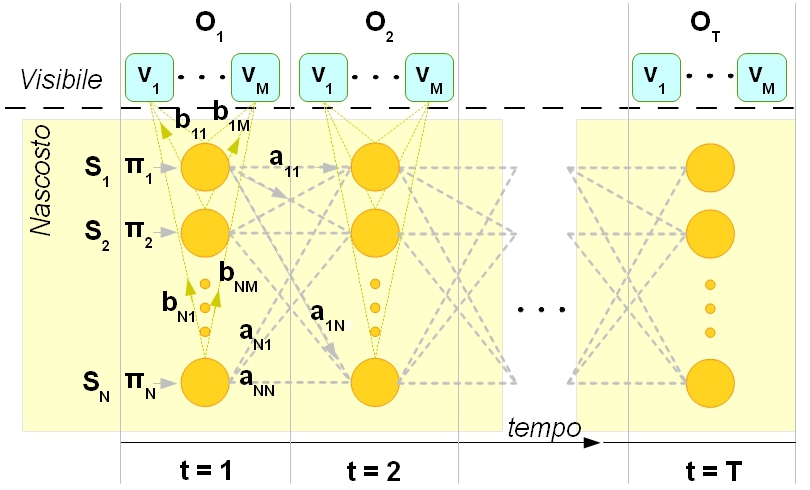
\includegraphics[width=1\textwidth]{imgs/descreteMarkovProcesses.jpg}
	\caption{Rappresentazione di un Processo di Markov Discreto generico, con una data sequenza di osservazioni $O_t$: un modello con $N$ stati nascosti ed $M$ possibili emissioni, $N$ probabilit� a priori $\pi_i$ (una per stato) a tempo $t = 0$, $N^2$ probabilit� di transizione tra stati $a_{ij}$ (per ciascuna coppia di stati $(S_i, S_j)$ con $i,j = 1,...,N$) per ogni unit� temporale $0 < t < T$ ed $(N \times M)$ probabilit� di emissione $b_{jk}$ (per ciascuna coppia stato - emissione $(S_i,v_k)$ con $i=1,...,N$ e $k=1,...,M$).}
	\label{fig:descreteMarkovProcesses}
\end{figure}

 Si pu� dare una descrizione probabilistica completa dei processi di Markov Discreti con la seguente equazione:

\begin{equation}
\wp [q_t = s_j | q_{t-1} = s_i, \ldots, q_0 = s_p]
\label{eq:fullProbDescription}
\end{equation}
Ovvero la probabilit� che il processo di Markov si trovi nello stato $s_j$ a tempo $t$ dato che a tempo $t-1$ si trovava nello stato $s_i$, e ..., e nello stato iniziale $q_0$ era nello stato $s_p$.
Un caso speciale di \eqref{eq:fullProbDescription} in cui la probabilit� che il sistema si trovi in un determinato stato nel presente dipende solo dall'istante di tempo precedente e non da tutta la storia a partire dal primo istante di tempo.

\begin{definition}[Modelli di Markov del Primo Ordine]
	\begin{equation}
		\wp[q_t = S_j | q_{t-1} = S_i]
		\label{eq:first_Order_MM}
	\end{equation}
\end{definition}

 Le Catene di Markov ad ogni istante temporale compiono una transizione di stato con una probabilit� nota. Tale probabilit� � descritta nella Matrice delle Probabilit� di Transizione.
\begin{definition}[Matrice delle Probabilit� di transizione]
	\begin{equation}
		A = a_{i,j} = \wp[q_t = S_j | q_{t-1} = S_i]\quad \text{con} 1 \leq i,j \leq N
		\label{eq:trans_prob}
	\end{equation}
\end{definition}

Propriet� delle $a_{ij}$ derivanti dal fatto che sono dei valori di probabilit�:
\begin{enumerate}
	\item $a_{ij}\geq 0$
	\item $\displaystyle\sum_{j=1}^{N}{a_{ij}}=1$
\end{enumerate}
All'istante di tempo iniziale $t = 0$, lo stato della Catena di Markov � determinato da una distribuzione di probabilit�. Un vettore $\pi: 1\times N$ che a ciascuno stato fa corrispondere la probabilit� che sia lo stato iniziale, questa � nota come probabilit� a Priori o probabilit� dello stato iniziale.

\begin{definition}[Distribuzione di probabilit� dello stato iniziale]
\begin{equation}
	\pi_i = \wp(q_1 = S_i) \quad \text{con} 1 \leq i \leq N
\label{eq:prior}
\end{equation}
  
\end{definition}


\section*{HMM}
\label{sec:HMM}
Avvolte le osservazioni sono funzioni probabilistiche di qualche stato nascosto (cio� esiste un processo stocastico  nascosto che produce una sequenza di osservazioni).  

%Il problema � come costruire un modello di marcoviano che le spieghi? 
%\TODO questo algoritmo fa veramente pena, valutare se mantenerlo
%\begin{algorithm}    
%\caption{Creare HMM}
%\label{alg:HMM_create}                                                  
%\begin{algorithmic}[1]                    
%WHILE{\COMMENT{modello = miglior spiegazione delle osservazioni}}
%	\STATE \COMMENT{Stabilire il numero di stati}
%	\STATE \COMMENT{Stabilire a cosa corrisponde ogni stato nella realt� }
%\ENDWHILE
%\RETURN \COMMENT{modello}
%\end{algorithmic}
%\end{algorithm}

\begin{definition}[Matrice di probabilit� delle Osservazioni]
\begin{equation}
\begin{split}
B &= \{b_j(k)\} \\
&\text{dove } b_j(k) = \wp[v_k \quad \text{all'istante } t | q_t = s_j] \quad \text{con } 1\leq j \leq N \quad , 1\leq k \leq M
\end{split}	 
\label{eq:emissionMtxDef}
\end{equation}
\end{definition}

\begin{definition}[HMM a Osservazioni discrete]
 \begin{equation}
	HMM = <N, M, A, B, \pi>
\label{eq:hmm}
\end{equation}
dove:
 \begin{enumerate}
	\item $N = |S|$ � l'insieme degli stati $S = \{s_1,\ldots, s_N\}$,
	\item $M = |V|$ � un insieme finito di Simboli di Osservazione $V = \{v_1, \ldots, v_M\}$ ,
	\item $A$ � la matrice di transizione definita in \eqref{eq:trans_prob},
	\item $B$ � la matrice di probabilit� dei Simboli di Osservazione definita in \eqref{eq:emissionMtxDef},
	\item $\pi$ � il vettore di probabilit� a priori definito in \eqref{eq:prior}.
\end{enumerate}
\end{definition}

Una HMM pu� essere usato per generare una sequenza di osservazioni $O=\{O_1,O_2,\ldots,O_T\}$ nel seguente modo:
\begin{algorithm}    
\caption{genera sequenze con HMM}
\label{alg:HMM_seq_gen}                                                  
\begin{algorithmic}[1]                    
	\STATE $q_1 = \displaystyle\arg\max_{1\leq i \leq N}{\pi_i}$
	\FOR{ $t = 1, \ldots, T ; t++$}
		\STATE $o_t = \displaystyle\max_{1 \leq s \leq N}[b_{{q_t},s}]$
		\STATE $q_t = \displaystyle\arg\max_{1\leq j \leq N}{a_{i,j}}$
	\ENDFOR	
\RETURN \COMMENT{modello}
\end{algorithmic}
\end{algorithm}
La Figura \ref{fig:HMM_seq_gen} da un intuizione sul funzionamento dell'algoritmo:
\begin{figure}[h]
	\centering
		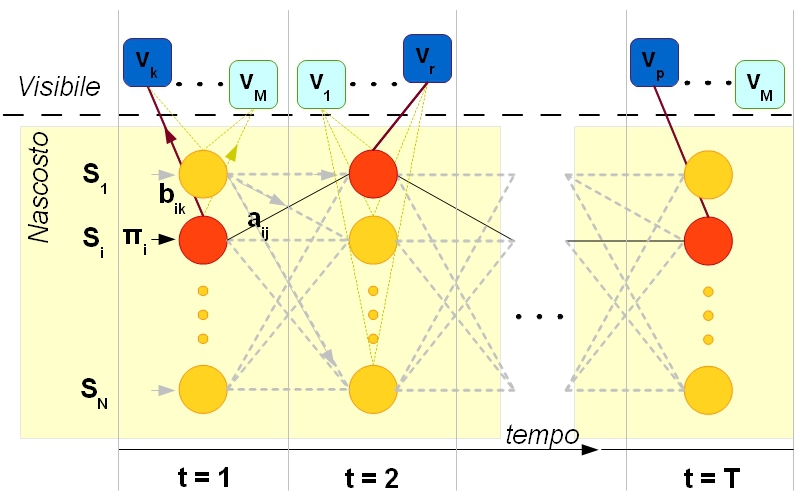
\includegraphics[width=1\textwidth]{imgs/descreteMarkovProcessesObservationGen.jpg}
	\caption{Esempio di generazione di una sequenza di osservazioni mediante l'Algoritmo \ref{alg:HMM_seq_gen}}
	\label{fig:HMM_seq_gen}
\end{figure}


\subsection*{HMM ad emissioni continue}
Nel caso in cui le osservazioni siano continue � necessario avere un modello che associ ad ogni stato una distribuzione di emissione, invece che un singolo valore. Un esempio di distribuzione � la gaussiana mono variata o ad una variabile (vedi Figura \ref{img:monovargaussian}). In questo caso la definizione della matrice di emissione descritta in \eqref{eq:emissionMtxDef} diventa
\begin{equation}
B = b_j(x) = \mathcal{N}(x,\mu_j,\sigma_j) = \frac{1}{\sigma_j\sqrt{2\pi}}\textbf{e} ^{-\frac{(x-\mu_j)^2}{2 \sigma_j^2}}\quad
\text{per} 1 \leq j \leq N
\label{eq:continuousEmissionMtx}
\end{equation}

\begin{figure}[h]
	\centering
		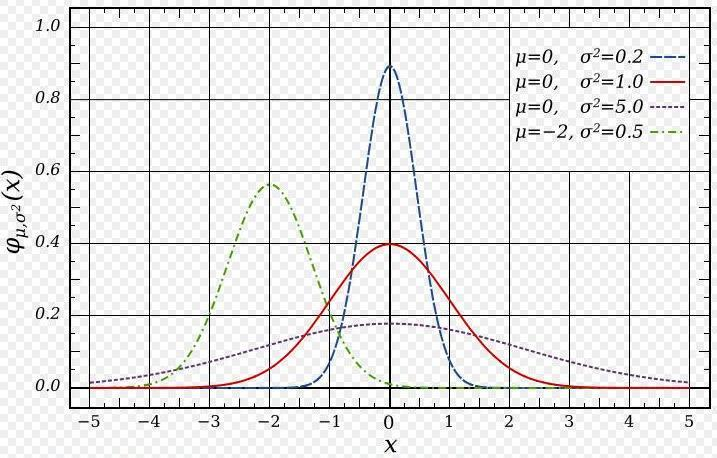
\includegraphics[width=.9\textwidth]{imgs/monovargaussian.jpg}
	\caption{Esempi di distribuzioni gaussiane monovariate.Immagine adattata da Wikipedia.}
	\label{fig:monovargaussian}
\end{figure}


La formula pu� essere generalizzata su due fronti: numero di variabili in ingresso: gaussiana mutivariata (vedi Figura \ref{bivargaussian}) oppure sul numero di gaussiane che vengono combinate: mistura di gaussiane (vedi Figura \ref{gaussianmixture}).

%\begin{figure}[h]
%	\centering
%		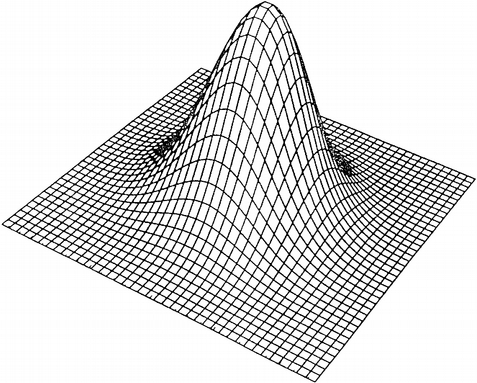
\includegraphics[width=.9\textwidth]{imgs/bivariategaussian.jpg}
%	\caption{Esempio di distribuzione gaussiana multivariata, in questo caso bivariata}
%	\label{fig:bivargaussian}
%\end{figure}

%\begin{figure}[h]
%	\centering
%		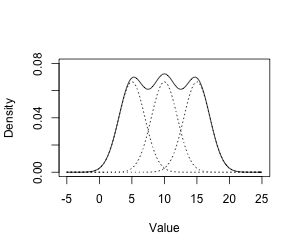
\includegraphics[width=.9\textwidth]{imgs/gaussianmixture.jpg}
%	\caption{Esempi di misture di gaussiane}
%	\label{fig:gaussianmixture}
%\end{figure}



\begin{equation}
B = b_j(x) = \displaystyle \sum_{m = 1}^{M} c_{j,m}\mathcal{N}(x,\bm\mu_j,\bm\Sigma_j)\quad \text{ per } 1 \leq j \leq N
\label{eq:continuousEmissionMtxGauusianMixtures}
\end{equation}

Ovviamente � possibile applicare qualunque tipo di distribuzione al posto della gaussiana.\\
Dalla definizione \eqref{eq:continuousEmissionMtxGauusianMixtures} segue 
\begin{equation}
\int_{-\infty}^{\infty}{b_j(x)}dx = 1 \quad \text{ per } 1 \leq j \leq N
\label{eq:contEmissGaussMixProperty}
\end{equation}


\subsection*{Tipi di HMM}
\label{sec:tipi_hmm}
Vi sono casi particolari di HMM che sono considerati importanti per la loro ricorrenza nella descrizione di sistemi naturali. 
Il pi� generico tipo di HMM � noto come Ergodico, in cui ogni stato � connesso ad ogni altro stato, quindi la matrice di transizione � una matrice senza zeri. \\
Un modello pi� significativo � il modello Bakis o Sinistra-Destra. In questo modello l'aumentare del tempo, causa una variazione monotona crescente modulo $N$ sull'indice degli stati. Questo modello � conforme ai segnali le cui propriet� variano con il tempo. Le matrici di transizione dei modelli Sinistra-Destra, godono della propriet�
\begin{equation}
\begin{split}
 a_{i,j} = 0 \quad \forall j < i\\
 a_{i,j} = 0 \quad j>i+\Delta
\end{split} 
\label{eq:bakisTransitionMtx}
\end{equation}
La seconda condizione serve ad evitare che vi siano grossi balzi in avanti sugli stati, di solito $\Delta = 2$.
Inoltre le probabilit� iniziali hanno il vincolo
\begin{equation}
\pi_i = 1 \Leftrightarrow i = 1
\label{eq:initial_prob_condition}
\end{equation} 
supponendo di avere gli stati ordinati da $1$ ad $N$

\section*[Tre problemi per le HMM]{Tipi di problemi che si affrontano con le HMM}

Generalmente con le HMM si affrontano 3 tipologie di problemi. 

\begin{enumerate}
	\item \textbf{Valutazione}: dati $O$ e $\lambda$, calcolare $\wp(O|\lambda)$ in modo ottimale.
	\item \textbf{Decodifica}: dati $O$ e $\lambda$, trovare la sequenza di stati $Q=q_1,q_2,\ldots, q_T$ ``migliore'', secondo un criterio di ottimalit�, che possa aver generato $O$.
	\item \textbf{Apprendimento}: dato $\lambda$, regolarne i parametri per massimizzare $\wp(O|\lambda)$?
\end{enumerate}


\subsubsection*{Valutazione} 
Il problema della valutazione (\textit{Evaluation}) consiste nel calcolare la probabilit� che una certa sequenza di osservazioni sia stata prodotta da un dato modello.\\
La soluzione del problema permette, dati diversi modelli candidati $\lambda_1, \ldots, \lambda_n$ ed una sequenza di osservazioni $O$, di scegliere $\lambda_k$ con $\displaystyle \max_{1\leq i \leq n}\{\wp(O|\lambda_i)\}$.\\

Una soluzione na�ve del problema della valutazione � quello di enumerare tutte le possibili sequenze di stati (detti anche percorsi)  $Q = q_1, \ldots, q_T$ dove $q_i \in S={s_1,s_2,\ldots, s_N}$ e calcolare per ciascuna la probabilit� che l'osservazione sia stata prodotta da essa e moltiplicare il risultato per la probabilit� che quel particolare percorso venga scelto.
\begin{equation}
\begin{split}
	\wp(O|\lambda) & = \displaystyle \sum_{1\leq t \leq T, i \in \{\text{tutti Q}\}}\wp(O_t|Q_i, \lambda)\wp(Q_i|\lambda) \quad \text{dove}\\
	& \wp(O|Q_i, \lambda)  =  \displaystyle \prod_{1\leq t \leq T} \wp(O_t|q_{i,t}, \lambda) \\ 	 
	& = b_{q_i,1}(O_1)*\ldots*b_{q_i,T}(O_T)\quad \text{e}\\
  & \wp(Q_i|\lambda)  =  \pi_{q_1}*a_{q_1,q_2}*\ldots *a_{q_T-1,q_T} 
\end{split}
\label{eq:naiveEvaluation}
\end{equation}

l'algoritmo ha complessit� esponenziale, $O(N^T)$.\\

La soluzione ottima a questo problema � data dall'algoritmo di programmazione lineare noto come algoritmo \textit{Forward}. L'idea su cui si basa � di considerare dei percorsi parziali per rappresentare osservazioni parziali. Vengono definite le variabili $\alpha_{i,t}$ come la probabilit� di aver osservato la sequenza parziale $O_1, \ldots, O_t$ e di essere nello stato $S_i$ all' istante temporale $t$ 
\begin{equation}
\alpha_{i,t} = \wp(o_1, \ldots, o_t, q_T=S_i|\lambda)
\label{eq:alpha}
\end{equation}

Dalla definizione \eqref{eq:alpha} ricaviamo la matrice $\alpha (N \times T)$ nella quale vengono inserite le probabilit� parziali per ogni combinazione stato-tempo, di modo che al passo temporale successivo il calcolo possa essere basato su tali valori e non ricalcolando tutto dal primo istante di tempo. 
\begin{algorithm}    
\caption{\textit{Forward}}
\label{alg:fwd}                                                  
\begin{algorithmic}[1]
\STATE {}\COMMENT{1. Inizializzazione}                    
\FOR{$j = 1$ to N=|S|} 
\STATE {$\alpha_{j,1}=\pi_j b_j(o_1)$\hspace{1.5cm}}\COMMENT{ \emph{La probabilit� congiunta di partire dal $j$-esimo stato} } 
\ENDFOR \hspace{4cm}\COMMENT{ \emph{ed emettere il primo segnale dallo stesso}} 
\STATE {}\COMMENT {2. Induzione}
\FOR{$t = 1$ to $T-1$} 
	\FOR{$j = 1$ to $N$ }
		\STATE {$\alpha_{j, t+1}=[\displaystyle\sum_{i=1}^N\alpha_{i,t}a_{i,j}]b_j(o_{t+1})$\hspace{.5cm}}
		 \COMMENT{ \emph{La probabilit� congiunta di arrivare al} } 	
		 \ENDFOR	\hspace{4cm}\COMMENT{ \emph{$j$-esimo stato ed emettere il $t+1$-esimo segnale}}
\ENDFOR
\STATE{}\COMMENT{3. Terminazione}
\FOR{$j = 1$ to $N$} 
	\STATE {$\wp(O|\lambda)=\displaystyle\sum_{j=1}^N \alpha_{j,T} $}
\ENDFOR
\end{algorithmic}
\end{algorithm}

La complessit� dell'algoritmo \textit{Forward} � $O(NT)$. Il netto miglioramento � dovuto al fatto che i risultati parziali vengono riutilizzati, limitando il numero di calcoli da svolgere ad ogni istante temporale a $N$. La struttura grafica su cui si basa l'algoritmo \textit{Forward} � detta struttura a traliccio. \\
  


\subsubsection*{Decodifica} 
Il secondo problema � noto come problema di Decodifica in cui si cerca la sequenza di stati $Q = q_1,\ldots,q_T$ che ha generato una data sequenza di osservazioni $O = o_1,\ldots, o_T$. Dato che, al contrario del problema della Valutazione, non esiste un'unica soluzione al problema di Decodifica, quello che si fa � di stabilire un criterio di ottimalit� in funzione del quale fare la ricerca. \\
Un possibile criterio di ottimalit� della sequenza � quello di scegliere gli stati $q_t$ che all'istante di tempo $t$ sono i pi� probabili. Tale criterio massimizza il numero atteso di stati corretti individualmente. \\
Per risolvere il problema necessitiamo di due variabili $\beta$ e $\gamma$. La prima � definita come risultato dell' algoritmo \textit{Backward}, che computa il processo inverso dell'algoritmo \textit{Forward}.

\begin{equation}
\beta_{i,t}=\wp(o_{t+1}\ldots o_T|q_t = S_i,\lambda)
\label{eq:beta}
\end{equation}


\begin{algorithm}    
\caption{\textit{Backward}}
\label{alg:bckwd}                                                  
\begin{algorithmic}[1]                    
\STATE {}\COMMENT{1. Inizializzazione}                    
\FOR{$j = 1$ to N=|S|} 
	\STATE {$\beta_{j,T} = 1$}
\ENDFOR
\STATE {}\COMMENT {2. Induzione}
\FOR{$t = T-1$ to $1$} 
	\FOR{$i = 1$ to $N$ }
		\STATE $\beta_{i,t}=\displaystyle\sum_{j=1}^N a_{i,j}b_j(o_{t+1})\beta_{j,t+1}$
	\ENDFOR
\ENDFOR
\end{algorithmic}
\end{algorithm}

La seconda variabile, $\gamma$ � definita come la probabilit� di essere in uno stato $S_i$ al tempo $t$, data un'osservazione $O$ ed un modello $\lambda$.
\begin{equation}
\gamma_{i,t} = \wp(q_t = S_i| O, \lambda)
\label{eq:gamma}
\end{equation}
$\gamma$ pu� essere calcolata in funzione delle variabili di \textit{Forward} e \textit{Backward}:

\begin{equation}
\gamma_{i,t} = \dfrac{\alpha_{i,t}\beta_{i,t}}{\wp(O|\lambda)} = 
							 \dfrac{\alpha_{i,t}\beta_{i,t}}{\displaystyle\sum_{j = 1}^N \alpha_{j,t}\beta_{j,t}}
\label{eq:gammaFnAlphaBeta}
\end{equation}

$\alpha_{i,t}$, fornisce le probabilit� delle osservazioni parziali fino a $t$, mentre $\beta_{i,t}$, da $t+1$ in poi, essendo correntemente nello stato $S_i$. Il denominatore dell'equazione \eqref{eq:gammaFnAlphaBeta} � un fattore di normalizzazione che rende $\gamma$ un valore di probabilit�, quindi sar� valida la propriet�
\begin{equation}
\displaystyle\sum_{i = 1}^N \gamma_{i,t} = 1
\label{eq:propriet�Gamma}
\end{equation}
 Usando $\gamma$ � possibile trovare lo stato $q$ che individualmente � il pi� probabile al tempo $t$:
\begin{equation}
q_t = \arg\max_{0 \leq i \leq N} \gamma_{i,t}
\label{eq:statoPi�Probabile}
\end{equation}

Anche se \eqref{eq:statoPi�Probabile} massimizza il numero di stati pi� probabili scegliendo quelli che individualmente sono i pi� probabili, potrebbe creare problemi nel momento in cui si considera una sequenza di stati. Se la HMM ha anche transizioni nulle, la sequenza generata da \eqref{eq:gammaFnAlphaBeta} potrebbe essere non valida, perch� non vi � nessun controllo sulla probabilit� di co-occorrenza di stati. \\
Il criterio di ottimalit� pu� essere cambiato ad individuare la miglior sequenza di lunghezza $T$ che massimizzi la probabilit� di tutti gli stati nella sequenza. Per trovare il cammino migliore, viene usato un metodo di programmazione dinamica detto algoritmo di Viterbi.
	L'algoritmo di Viterbi individua la migliore sequenza di stati che rispondano a una data sequenza di osservazioni: \begin{equation}
\delta_{i,t} = \max_{q_1,\ldots q_{t-1}}\wp(q_1 \ldots q_t = S_i,o_1 \ldots o_t|\lambda)\\
\label{eq:delta}
\end{equation}

Nella matrice $\delta$ vengono inserite le probabilit�, mentre per tenere traccia del percorso migliore si usa una variabile $\psi$:
\begin{equation}
\psi_{i,t} = \arg\max_{q_1,\ldots q_{t-1}}\wp(q_1 \ldots q_t=i,o_1 \ldots o_t|\lambda)
\label{eq:psi}
\end{equation}

La procedura completa per trovare il percorso di stati pi� probabile � la seguente:
\begin{algorithm} 
\caption{Viterbi}
\label{alg:viterbi}                                                  
\begin{algorithmic}[1]                    
\STATE{}\COMMENT{Inizializzazione}
\FOR {$i = 0$ to $N$}
	\STATE {$\delta_{i,1} = \pi_i b_i(o_1)$}
	\STATE {$\psi_{i,1} = 0$}
\ENDFOR
\STATE{}\COMMENT{Iterazione}
\FOR{$t = 2$ to $T$}
	\FOR{$i = 1$ to $N$} 
		\STATE $ \delta_{i,t}=\displaystyle\max_{1\leq j \leq N} [\delta_{j,t-1}a_{j,i}]* b_i(o_i)$
		\STATE $ \psi_{i,t}=\displaystyle\arg \max_{1\leq j \leq N} [\delta_{j, t-1}a_{j,i}]$
	\ENDFOR
\ENDFOR
\STATE{}\COMMENT{Terminazione}
\STATE $P* = \displaystyle \max_{1\leq i \leq N} [\delta_{i,T}]$
\STATE $q_T* = \displaystyle \arg \max_{1\leq i \leq N} [\delta_{i,T}]$
\STATE{}\COMMENT{Backtracking}
\FOR{$t=T-1$ to $1$}
	\STATE{$q*_t=\psi_{q*_{t+1},t+1}$}
\ENDFOR
\end{algorithmic}[1]
\end{algorithm}
	
	
\subsection*{Algoritmo di Viterbi in Tempo Reale}	
Il problema dell'algoritmo di Viterbi in molte applicazioni reali, � la latenza. I sistemi che utilizzano l'algoritmo hanno spesso necessit� di avere risultati immediati, in tempo reale. Trovare la sequenza di stati pi� verosimile che ha generato una sequenza di osservazioni � (come mostrato dall'Algoritmo \ref{alg:viterbi}) fattibile con l'algoritmo di Viterbi, tracciando percorsi nella sequenza temporale di stati ed una volta arrivato a termine (tempo finale $T$), ricostruendo a ritroso il cammino migliore. Un problema significativo dell'algoritmo � che assume che la sequenza temporale sia finita. Vi sono molti casi pratici in cui l'applicazione dell'algoritmo sarebbe utile, per i quali i dati sono un flusso continuo ed incessante di dati. Una possibile soluzione � l'applicazione del'algoritmo di Viterbi a finestre successive di dati, dopo la quale restituire solo una parte iniziale degli decodificati  \cite{synface_low_latency_viterbi}, \cite{automatic_bass_line_transcript}(perch� hanno una probabilit� maggiore di essere corretti). Questa soluzione, conduce a una decodifica sub-ottimale.\\
Un'altra soluzione consiste nel confrontare pi� percorsi su una finestra temporale in espansione, finch� le soluzioni non convergono. Nel lavoro \cite{real_time_viterbi_optimization_multi_target_tracking} per la localizzazione automatica di un soggetto via video, la finestra temporale viene dinamicamente ridimensionata in base a un'euristica che bilanci latenza e accuratezza. Questo tipo di approccio non garantisce la convergenza dei percorsi considerati. L'approccio che noi abbiamo usato nel lavoro � quello proposto da Bloit et al \cite{short_time_viterbi_online_hmm_deconding}. 

\begin{definition}[Cammino locale]
Viene detta cammino locale, la sequenza di stati $s(a,b,i)$ ottenuta applicando l'algoritmo di Viterbi alla finestra temporale dall'istante temporale $a$ all'istante $b$ (con $a < b$) e compiendo il backtracking da uno stato arbitrario $i$ al tempo $b$. 
\end{definition}

\begin{definition}[Punto di Fusione]
Si definisce punto di fusione,l'istante temporale $\tau < T$  t.c per $a \leq t \leq \tau$, tutti i cammini locali appartenente all'insieme dei cammini locali $CL =\{ s(a,b,i), \forall i \in S\}$ (dove $S$ � l'insieme degli stati dell'HMM), sono uguali.
\end{definition}
	
Un punto di fusione gode della seguente propriet�:
i cammini locai fino al punto di fusione (che per definizione sono tutti uguali) sono sempre uguali al cammino globale (quello ottenibile con l'Algoritmo di Viterbi originale \ref{alg:viterbi})\footnote{per la dimostrazione consultare \cite{short_time_viterbi_online_hmm_deconding}}.

%\begin{algorithm} 
%\caption{ShortTimeViterbi}                                                  
%\label{alg:short_time_viterbi_decoding}   


\begin{algorithmic}
\STATE{$a = 0$, $b = 0$ }
%\FOR {ogni finestra temporale al tempo $b$}
%	\STATE calcola  $s_t(a,b,i) \forall I \in (a,b,\lambda)$
%	\IF{se viene trovato punto di fusione $\tau > a $}
%	\STATE risultato = $s*_{a,\tau}$
%	\STATE $a = \tau$
%\ENDFOR
\end{algorithmic}
%\label{alg:short_time_viterbi_decoding}   


	
\subsubsection* {Apprendimento}
L'ultimo problema � quello dell'Apprendimento che consiste nel configurare i parametri di $\lambda$ per massimizzare la probabilit� di una sequenza di dati osservati. Non � noto un metodo analitico per risolvere il problema, infatti, data una sequenza finita di osservazioni, non esiste un modo ottimo di stimare i parametri di $\lambda$. Possiamo per� scegliere $\lambda$ in modo da massimizzare localmente $\wp(O|\lambda)$, con un procedimenti iterativi come 
\begin{itemize}
	\item Baum-Welch
	\item Expectation-Modification
	\item Tecniche basate sul gradiente
\end{itemize}
La procedura iterativa � detta riestimazione, e consiste in un miglioramento graduale (in base ad un criterio) ed un aggiornamento dei parametri. Per descrivere le riestimazione, � necessario definire la variabile $\xi$ come la probabilit� di essere in un certo stato in un istante di tempo ed essere in un altro nel successivo istante di tempo:
\begin{equation}
\begin{split}
\xi_t(i,j) &= \wp(q_t = S_i, q_{t + 1} = S_j|O,\lambda)\\
					 &= \displaystyle \dfrac{\alpha_{i,t} a_{i,j}b_i(o_t)\beta_{j, t+1}}{\wp(O|\lambda)}=
\displaystyle \dfrac{\alpha_{i,t} a_{i,j}b_i(o_t)\beta_{j, t+1}}{\displaystyle\sum_{i=1}^{N}\sum_{j=1}^{N}\alpha_{i,t} a_{i,j}b_i(o_t)\beta_{j, t+1}}
\label{eq:xi}
\end{split}
\end{equation}

Possiamo correlare $\gamma$ e $\xi$ nel seguente modo
\begin{equation}
\gamma_{i,t} = \displaystyle\sum_{j=1}^N \xi_t(i,j)
\label{eq:gammaxi}
\end{equation}

\begin{definition}{Numero di transizioni attese}\\
\begin{itemize}
	\item Numero di transizioni attese da $S_i$
		\begin{equation}
			\displaystyle \sum_{t=1}^{T-1} \gamma_{i,t}
			\label{eq:numTransizAtteseDa}
		\end{equation}
	\item Numero di transizioni attese da $S_i$ a $S_j$
		\begin{equation}
			\displaystyle \sum_{t=1}^{T-1} \xi_t(i,j)
			\label{eq:numTransizAtteseDaA}
		\end{equation}
	\item $\overline{\pi}_i$ = numero di volte nello stato $S_i$ a tempo $t = 1$ atteso 
			\begin{equation}
					= \gamma_{i,1}
			\label{eq:piGamma}
			\end{equation}
	\item	$\overline{a}_{i,j} =\displaystyle \dfrac{\text{numero di transizioni attese dallo stato} S_i \text{allo stato} S_j}
																								 {\text{numero di transizioni attese dallo stato} S_i}$
			\begin{equation}
					= \displaystyle\dfrac{\displaystyle\sum_{t=1}^{T-1}\xi_t(i,j)}
														  {\displaystyle\sum_{t=1}^{T-1}\gamma_{i,t}}
			\label{eq:transitionMtxXi}
			\end{equation}																								 
																							
	\item $\overline{b}_j(k) =\displaystyle \dfrac{\text{numero di volte nello stato} S_j \text{osservando} v_k}
																								 {\text{numero di volte atteso nello stato} S_i}$
			\begin{equation}
					= \displaystyle\dfrac{\displaystyle\sum_{t=1	}^{T}\gamma_{j,t}\quad \text{t.c. $o_t = v_k$}}
														  {\displaystyle\sum_{t=1}^{T}\gamma_{j,t}}  
			\label{eq:emissionMtxGamma}
			\end{equation}				 
\end{itemize}
\end{definition}

Dato il modello $\lambda = (A,B,\pi)$ indico il modello riestimato con $\overline{\lambda} = (\overline{A},\overline{B},\overline{\pi})$. L.Baum et al\cite{maximization_technique_stat_analysis_fun_markov_ch} hanno dimostrato che nel processo di riestimazione � vera una delle seguenti alternative:
\begin{enumerate}
	\item $\lambda = \overline{\lambda}$
	\item $ \wp(O|\overline{\lambda}) > \wp(O|\lambda)$
\end{enumerate}

Nel secondo caso � possibile sostituire $\overline{\lambda}$ a $\lambda$, ripetendo l'iterazione, finch� non si verifica una condizione d'arresto, ed il risultato della procedura � detto stima di massiva verosimiglianza (\textit{maximum likelihood estimate}) dell'HMM
\begin{algorithm}    
\caption{Baum-Welsh o \textit{Maximum Likelihood Expectation}.  }
\label{alg:baum_welsh}                                                  
\begin{algorithmic}[1]                   
\REQUIRE{maxlikelihood($\lambda = A,B,\pi$)}
\REPEAT 
	\STATE{\fbox{$\pi_i=\gamma_1(i)$}
		\fbox{{$a_{ij}=\dfrac{\displaystyle\sum_{t=1}^{T-1}\xi_t(i,j)}{\displaystyle\sum_{t=1}^{T-1}\gamma_t(i)}$}}
		\fbox{$b_j(k)=\dfrac{\displaystyle\sum_{t=1, O_t=V_k}^{T}\gamma_t(j)}{\displaystyle\sum_{t=1}^{T}\gamma_t(j)}$}}
	\IF{$\lambda=\tilde{\lambda}$}
		\RETURN{$\lambda$}
	\ELSIF{$\wp(O|\tilde{\lambda})>\wp(O|\lambda)$}
		\STATE maxlikelihood$(\tilde{\lambda})$
	\ENDIF
\UNTIL{\COMMENT{una condizione limite}}
\end{algorithmic}
\end{algorithm}



\section*{Problemi di implementazione di HMM}
Vi sono diversi problemi che si devono affrontare per implementare le HMM ed i vari algoritmi sinora descritti. Alcuni di questi sono 
\begin{itemize}
	\item Ridimensionamento (\textit{scaling}): la procedura di riestimazione, comporta una lunga sequenza di prodotti di valori di probabilit�. Ci� fa in modo che i valori tendano esponenzialmente a zero, quindi vi � un inevitabile problema di underflow. L'unico modo di ovviare al problema � quello di ridimensionare i valori, moltiplicandoli per un coefficiente che non dipenda dallo stato, ma solo dal tempo. Alla fine del processo, i coefficienti di ridimensionamento vengono eliminati.  \\
	Ad esempio nella procedura di riestimazione si calcola la matrice di transizione con l'Equazione \eqref{eq:transitionMtxXi}
		\begin{equation}
				\overline{a_{i,j}}= \dfrac{\displaystyle\sum_{t=1}^{T-1}\alpha_{i,t}a_{i,j}b_j(o_{t+1})\beta_{j,t+1}}													{\displaystyle\sum_{t=1}^{T-1}\displaystyle\sum_{j=1}^{N}\alpha_{i,t}a_{i,j}b_j(o_{t+1})\beta_{j,t+1}}
		\label{eq:transitionMtxAlphaBeta}
		\end{equation}
		
	Usando un coefficiente di ridimensionamento � $c_t = $
	\begin{equation}
			\frac{1}{\displaystyle\sum_{j=1}^{N}\alpha_{i,t}}
	\label{eq:scaleFactorOForAlpha}
	\end{equation}
	si ottiene un $\alpha_{j,t}$ scalato 
	\begin{equation}
		\hat{\alpha}_{j,t} = \dfrac{\displaystyle\sum_{j=1}^N \hat{\alpha}_{j,t-1}a_{i,j}b_j(o_t)}
		{\displaystyle\sum_{i=1}^{N}\displaystyle\sum_{j=1}^{N}\hat{\alpha}_{i,t-1}a_{i,j}b_j(o_{t})}
	\label{eq:scaledAlpha}
	\end{equation}
	Nel momento in cui vengono calcolati i $\beta_{j,t}$, vengono eliminati i fattori di ridimensionamento:
	\begin{equation}
			\hat{\beta}_{j,t} = c_t\beta_{j,t}
	\label{eq:scaledBeta}
	\end{equation}
	
	La modifica pi� importante deve essere applicata all'algoritmo \textit{Forward}, perch� si � interessati al valore di probabilit�. In questo caso non � possibile semplicemente sommare $\hat{\alpha_{j,t}}$, perch� sono valori scalati e privi di significato se presi singolarmente. In questo caso viene usata la seguente propriet�:
	\begin{equation}
		\begin{split}
			\prod_{t=1}^T c_t \displaystyle \sum_{i=1}^N \alpha_{i,T}& = 1\\
			\prod_{t=1}^T c_t \wp(O|\lambda) &= 1 \Leftrightarrow \wp (O|\lambda) = \frac{1}{\prod_{t=1}^T c_t}
		\end{split}
	\label{eq:propriet�Alpha}
	\end{equation}
	Qui introduciamo il logaritmo della probabilit�, in modo che il valore sia calcolabile su un computer
	\begin{equation}
		\log (\wp(O|\lambda)) = -\displaystyle\sum_{t=1}^T \log c_t
	\label{eq:logLikelihood}
	\end{equation}
	\item Molteplici sequenze di osservazione. Nelle HMM Sinistra-Destra, non si possono usare singole sequenze di osservazioni per addestrare il modello, perch� questo tipo di modello tende a uscire molto facilmente da uno stato, quindi ad ogni stato corrispondono pochissime osservazioni. Ci� implica che per una quantit� di dati sufficiente a fare una stima affidabile dei parametri del modello si devono usare pi� sequenze di osservazioni.  
	\item Stime dei parametri iniziali. Un problema irrisolto � come scegliere i valori dei parametri iniziali in modo tale che i massimi locali corrispondano al massimo globale della funzione di verosimiglianza (likelihood). Normalmente quello che si fa � scegliere valori casuali oppure uniformi per poi iniziare la procedura di riestimazione. Invece per quanto riguarda i parametri $B$ � necessaria una buona stima iniziale, che solitamente viene fatta con un processo di segmentazione e media delle osservazioni in stati. 
	\item Insufficienza di dati. Un problema frequente � che il numero di osservazioni � troppo basso per consentire di avere una stima abbastanza buona dei parametri del modello. Una possibile soluzione � quella di aumentare il numero di dati, ma ci� � spesso impraticabile. L'approccio inverso � quello di ridurre il numero di parametri, come ad esempio il numero di stati. Ci� � in teoria sempre praticabile, ma spesso poco sensato, in quanto vi sono delle motivazioni valide per avere quei parametri. Una terza alternativa � quella di interpolare tra un insieme di stime di parametri con un'altro da un modello per il quale si ha un numero sufficiente di dati di addestramento. L'idea � quella di progettare insieme al modello, anche una versione ridotta dello stesso, per il quale il numero di dati in possesso sia sufficiente. Date le stime per i parametri del modello $\lambda = (A,B,\pi)$ come per la versione ridotta $\lambda' = (A',B',\pi')$ il modello interpolata � ottenuto come
	\begin{equation}
		\tilde{\lambda} = \epsilon \lambda + (1- \epsilon)\lambda'
	\label{eq:modelInterpolation}
	\end{equation}
	dove $\epsilon$ rappresenta un peso che viene associato ai parametri del modello, ed $(1- \epsilon)$ il peso associato a quelli del modello ridotto. Il valore di $\epsilon$ viene determinato in funzione dei dati di addestramento. Mercer et al \cite{interpolation_markov_params_sparse_data} hanno dimostrato che � possibile stimare l'$\epsilon$ ottimo mediante l'algoritmo \textit{Forward}-\textit{Backward}, espandendo la HMM a partire da \eqref{eq:modelInterpolation}.
	\item Scelta della dimensione e tipo del modello. Si tratta della scelta dei parametri che si deve fare all'inizio per rappresentare al meglio il problema con le HMM. Il tipo di HMM, Ergodico o Sinistra-Destra, la dimensione del modello  cio� numero di stati, l'alfabeto di osservazione, discreti o continui, a distribuzione singola o a misture di distribuzioni. Non vi � un metodo standard, o migliore di prendere queste decisioni, ma devono essere fatte in base al tipo di segnale che si sta modellando.
\end{itemize}

\chapter[Tempo Reale, In Linea, Latenza]{Sistemi in Tempo Reale, algoritmi in Linea ed il problema della latenza e accuratezza}
\label{sec:real_time_sys}
La seguente sezione fornisce un chiarimento sul concetto di tempo reale, che spesso viene usato, anche in letteratura, in modo errato per intendere in linea. L'algoritmo di segmentazione usato in questo lavoro � un algoritmo in linea, non in tempo reale.
\section*{Tempo Reale}
La nozione di Tempo Reale (\textit{Real Time}, RT) si contrappone ad una di tempo logico o virtuale, in quanto misura di una quantit� fisica. La seconda forma di tempo, quella logica, � una misura di tipo qualitativo e rappresenta l'ordine di eventi.\\

In diversi ambiti, la nozione di sistema RT assume significati diversi:

\par\textsc{Informatica}: si parla di Computazione RT (\textit{Real Time Computing} - RTC) o computazione Reattiva: lo studio di sistemi software e hardware soggetti a vincoli di tempo reale. Un esempio di tale sistema sono i sistemi operativi RT (un esempio � LynxOS), che garantiscono tempi di risposta ben definiti, a differenza dei sistemi operativi non RT (anche se solitamente hanno tempi di risposta brevi).\\
Un altro esempio sono i linguaggi di programmazione Sincroni come ChucK, che � un linguaggio concorrente per l'elaborazione di file audio.
\par\textsc{Simulazioni}: RT si riferisce ad una sincronizzazione con le tempistiche reali, ovvero gli eventi nel processo simulato devono avvenire allo stesso tempo degli eventi nel processo reale. Un esempio sono i video giochi.
\par\textsc{Trasferimento di dati ed elaborazione di media}: RT assume un significato pi� soggettivo che riflette la percezione dell'utente finale, significa senza un ritardo percettibile dall'utente.



Sistemi RT possono essere classificati in base alla conseguenza di un ritardo nei tempi di risposta.
	\par\textsc{Sistemi Hard RT}: Un ritardo pu� avere delle conseguenze catastrofiche, ad esempio un sistema di pilotaggio.
	\par\textsc{Sistemi Soft RT}: Un ritardo non ha conseguenze sulla vita o di tipo economico, ad esempio un sistema per la visualizzazione di file video.

Per garantire che tali scadenze vengano rispettate, deve essere noto il tempo di esecuzione massima dei singoli processi 
di un programma. Questo problema � molto complesso e spesso si ottengono solo soluzioni parziali.\\

\section*{Algoritmi in linea}
\label{sec:online}
Un algoritmo � detto in linea (\textit{online}), se � in grado di dare un risultato a partire da un sottoinsieme di dati in ingresso in un determinato ordine. Un algoritmo fuori linea (\textit{offline}) invece, deve avere tutti i dati inizialmente per poter fornire un risultato.\\ Esempi dei due tipi di algoritmi sono l'algoritmo di ordinamento a inserzione (\textit{Insertion Sort}) che ha bisogno di 1 numero in pi� alla volta per poter fornire dopo n esecuzioni una lista ordinata, mentre l'algoritmo di ordinamento per selezione (\textit{Selection Sort}) ha bisogno dell'intera lista di numeri per poter cominciare a ordinare. \\

Dato che un algoritmo in linea prende decisioni basate solo su parte dei dati di cui necessiterebbe la risoluzione del problema in questione, le decisioni prese possono risultare non ottimali. Uno degli obbiettivi dello studio degli algoritmi in linea � di valutare la qualit� delle decisioni possibili in tali circostanze. 
Il metodo che viene utilizzato per formalizzare questa idea � noto come Analisi Competitiva: vengono confrontate le prestazioni relative di un algoritmo in linea e fuori linea ottimale sulla stessa istanza di un problema.\\

\section*{Latenza}
Il concetto di latenza nell'ambito informatico/ingegneristico assume svariati significati. Generalmente fa riferimento ad un ritardo rispetto ad un tempo atteso in un sistema. 
Un significato di latenza che si vuole menzionare in questo lavoro � quella dell'ambito biomedico: la latenza di un sistema di misurazione clinica dal punto di vista di un fisiatra � il ritardo sul tempo di risposta positiva. Nel caso di un segmentatore di deambulazione, la latenza � la differenza tra il tempo in cui si verifica un evento ed il tempo in cui il sistema annuncia l'avvenimento dell'evento. Ci� significa che i risultati errati aumentano la latenza. Quindi un sistema ha una latenza bassa, non solo se ha tempi di risposta brevi, ma ha anche un alta percentuale di risultati corretti. 
\chapter{Cenni di Meccanica classica}
\label{meccanica_classica}
La Meccanica classica � una delle due branche maggiori della Meccanica, che si occupa di leggi che descrivono il moto di corpi sotto l'azione di un sistema di forze \cite{Wikipedia}.

\section*{Cinematica}
La Cinematica \cite{Douglas_classical_mechanics} � lo studio del moto di corpi materiali, senza considerare le cause e conseguenze di tale moto. La parte della Meccanica che si occupa delle cause e conseguenze del moto dei corpi � la Dinamica o Cinetica. La Cinematica fornisce una descrizione geometrica dei possibili moti.\\
Il soggetto mediante il quale vengono condotti gli studi in Cinematica � la particella, vale a dire un corpo immaginario, che occupa un singolo punto dello spazio. Un insieme di particelle le cui distanze relative rimangono invariate in ogni riferimento spaziotemporale. 

\subsection*{Moto rettilineo di una particella}

Data una particella in moto rettilineo uniforme (vedi Figura \ref{fig:CinematicaLineare}), il suo moto pu� essere descritto secondo le seguenti quantit�:
\begin{description}
	\item[Posizione] Il vettore posizione della particella $P$ nel punto A
	
\begin{equation}
\begin{split}
\mathbf{r} & = (x_A,y_A,z_A) \quad \text{vettore posizione}\\
|\mathbf{r}| & = \sqrt{x_A^2 + y_A^2 + z_A^2}(m) \quad \text{magnitudine}
\end{split}
\label{eq:positionVector}
\end{equation}


	 

\item[Spostamento] Lo spostamento da $A$ a $B$ di $P$:

\begin{equation}
\begin{split}
\mathbf{r}_{AB} = \mathbf{r}_{B} - \mathbf{r}_{A} (m)
\end{split}
\label{eq:displacement}
\end{equation}


\item[Distanza] La distanza 

\begin{equation}
\begin{split}
\displaystyle s=\int_{t_1}^{t_2}{\sqrt{\Big(\dfrac{dx}{dt}\Big)^2 + \Big(\dfrac{dy}{dt}\Big)^2+ \Big(\dfrac{dz}{dt}\Big)^2}dt} (m)\\
\end{split}
\label{eq:distance}
\end{equation}
dove $t$ � il tempo.


\item[Velocit�] 

	\begin{itemize}
		\item media 
\begin{equation}
\begin{split}
\mathbf{\bar{v}} = \dfrac{\Delta \mathbf{r}}{\Delta t}(m/s)\quad \Delta t > 0
\end{split}
\label{eq:averageSpeed}
\end{equation}
				
		\item istantanea 

			\begin{equation}
				\begin{split}
					\mathbf{v} &= \displaystyle \lim_{\Delta t \rightarrow 0} \dfrac{\Delta \mathbf{r}}{\Delta t}\\
					|\mathbf{v}| &= \dfrac{ds}{dt}(m/s)\quad \text{magnitudine}
				\end{split}
			\label{eq:instantSpeed}
			\end{equation}
	
	\end{itemize}
	
\begin{figure}[h]
	\centering
		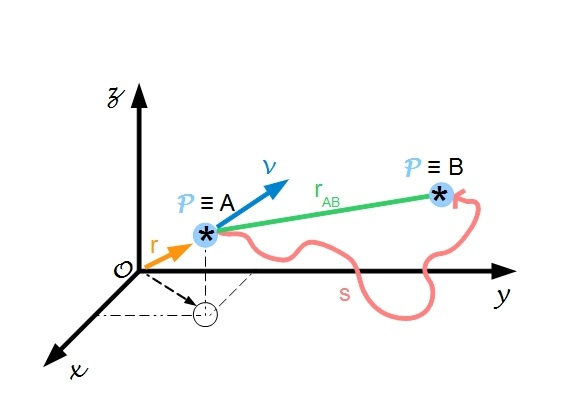
\includegraphics[width=.80\textwidth]{imgs/CinematicaLineare.jpg}
	\caption{Moto Rettilineo di una particella}
	\label{fig:CinematicaLineare}
\end{figure}
	
\item[Accelerazione]
	\begin{itemize}
		\item media 
			\begin{equation}
				\begin{split}
					\mathbf{\bar{a}} = \dfrac{\Delta \mathbf{v}}{\Delta t} \quad \Delta t > 0 (m/s^2)
				\end{split}
			\label{eq:instantSpeed}
			\end{equation}		
		\item istantanea 
			\begin{equation}
				\begin{split}
					\mathbf{a} = \displaystyle \lim_{\Delta t \rightarrow 0} \dfrac{\Delta \mathbf{v}}{\Delta t}(m/s^2) 
				\end{split}
			\label{eq:instantSpeed}
			\end{equation}
	\end{itemize}
\end{description}	

\section*{Moto Angolare di una particella}
Data una particella in moto circolare uniforme (vedi Figura \ref{fig:CinematicaAngolare}), il suo moto pu� essere descritto secondo le seguenti quantit�:
\begin{description}
	\item[Posizione] Il vettore posizione della particella $P$ nel punto $A$ rispetto ad un asse di rotazione $O-z$ � $\mathbf{r}(t)$. La posizione angolare del punto $P$ �
			\begin{equation}
				\begin{split}
	  \mathbf{r}_{\perp}(t) = r_{\perp x} \cos \theta i + r_{\perp x} \sin \theta j (rad)
				\end{split}
			\label{eq:angularPositionVector}
			\end{equation}
	 


\item[Velocit�] 
La velocit� angolare � data da: 
		$\omega = \dfrac{d\theta}{dt}$ $(rad/s)$
	\begin{figure}[h]
	\centering
		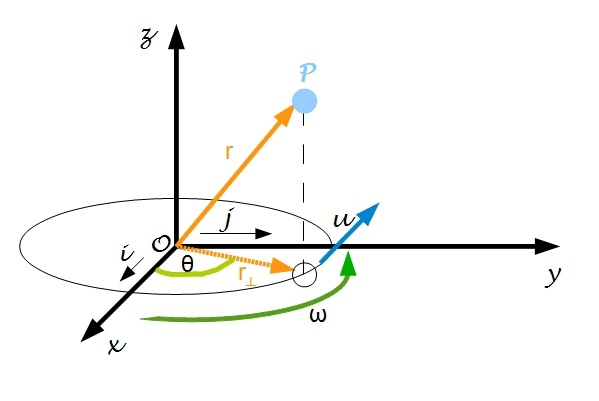
\includegraphics[width=.80\textwidth]{imgs/CinematicaAngolare.jpg}
	\caption{Moto Angolare di una particella}
	\label{fig:CinematicaAngolare}
\end{figure}
	
\item[Accelerazione]
L'accelerazione angolare � data da:
			\begin{equation}
				\begin{split}
					\alpha = \dfrac{d\omega}{dt}(rad/s^2)
				\end{split}
			\label{eq:acceleration}
			\end{equation}
\end{description}	
	
\section*{Dinamica (Cinetica)}
Branca della meccanica che si occupa di forze che producono, arrestano o modificano il moto di corpi. 
Le due leggi fondamentali della Dinamica sono quelle di Newton, in particolare la seconda �:
\begin{equation}
F = ma
\label{eq:secondoPrincipioNewton}
\end{equation}
\chapter{Sensori}
%\myChapter{Sensori}
\label{sec:sensori}
Principalmente in questo lavoro usiamo un giroscopio monoassiale. In letteratura, l'analisi della deambulazione viene 
affrontata mediante accelerometri, giroscopi e magnetometri. 
\section*{Accelerometro}
\label{sec:accelerometer}
Un accelerometro (vedi figura \ref{fig:acc}) � un dispositivo elettromeccanico che misura le forze di accelerazione. Tali forze possono essere sia statiche, come la forza di gravit�, che dinamiche, causate muovendo l'accelerometro.\\
Gli usi immediati di un accelerometro sono 
\begin{itemize}
	\item misurando l'accelerazione statica delle forza di gravit�, si pu� calcolare l'angolo a cui � inclinato lo strumento.
	\item misurando l'accelerazione dinamica si pu� analizzare il modo in cui si sta muovendo il dispositivo  
\end{itemize}
Un applicazione industriale importante � l'airbag nelle macchine, la cui apertura scatta se l'accelerometro percepisce una brusca frenata.
Un'altra applicazione � quella implementata dalla Apple, nei suoi portatili per la protezione del disco rigido: se il portatile dovesse cadere mentre acceso, l'accelerometro capta la caduta libera ed il sistema operativo si auto termina immediatamente in modo che la testina non sia sul disco. 

\begin{figure}
	\centering
	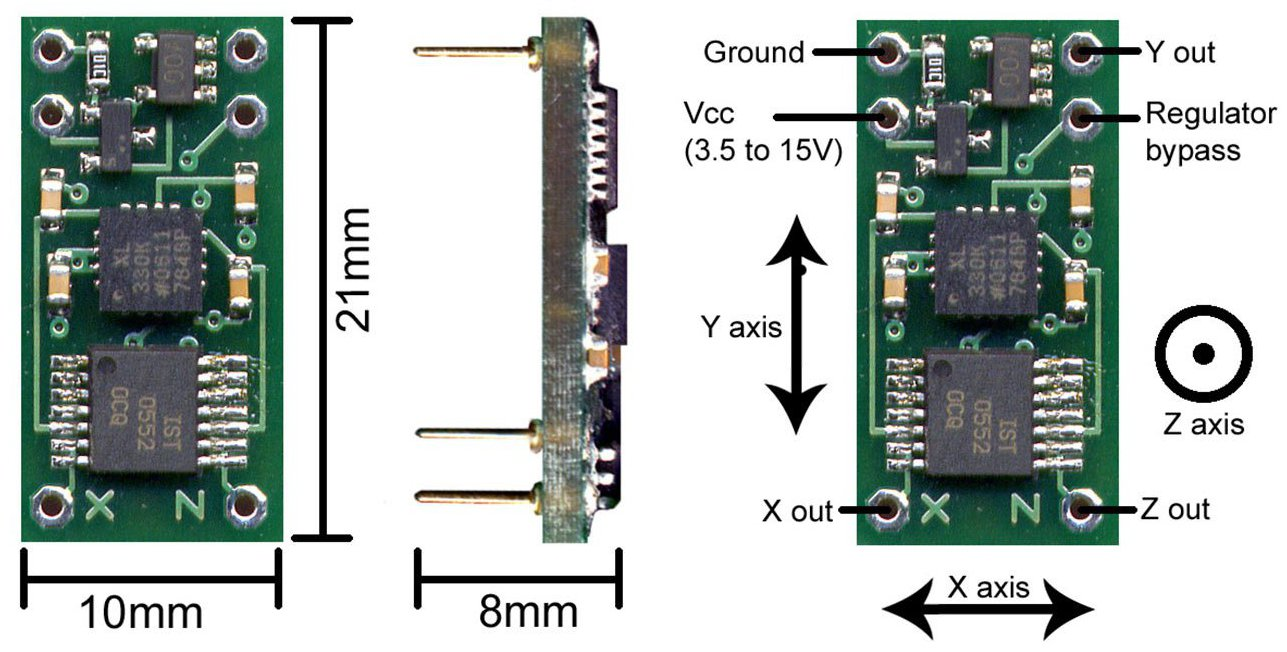
\includegraphics[width=1\textwidth]{imgs/acc_technical.jpg}
	\caption{ Accelerometro triassiale, cortesia di \url{http://www.dimensionengineering.com}}
	\label{fig:acc}
\end{figure}

\section*{Giroscopio}
\label{sec:gyroscope}
Il giroscopio � uno strumento per misurare l'accelerazione di rotazione (momento angolare) di un corpo. Vi sono diversi tipi di giroscopi, meccanici, a vibrazione, a fibre ottiche ecc..
Un disco rotante in assenza di torsione esterna, mantiene la direzione della sua rotazione 
 Quando viene applicata una torsione viene applicata al disco, ad angolo con il suo asse di rotazione, il disco ruota sul piano determinato dalle due assi (rotazione iniziale e torsione) nella direzione che va dall'asse di rotazione iniziale a quello della torsione.\\
Il tipo di giroscopio che usiamo in questo lavoro � il cosiddetto giroscopio piezoelettrico, o MEMS (Micro Electro Mechanical System) o a vibrazione. Si basa sul principio di Coriolis: un oggetto che vibra, continua a vibrare sullo stesso piano se la struttura che lo sostiene � in rotazione. 
La misurazione della velocit� angolare avviene nel seguente modo: un elemento piezoelettrico (oggetto di forma tubolare) oscilla a causa di una rotazione, quindi viene misurata la forza di Coriolis sulla sezione longitudinale dell'elemento, dopo essere stata convertita in un voltaggio elettrico dallo stesso elemento piezoelettrico. 
 
\section*{Magnetometro}
\label{sec:magnetomerter}
Il Magnetometro � uno strumento che misura il campo magnetico. Questo pu� essere fatto in diversi modi. Il metodo pre elettronico, � quello inventato da Coulomb ed usa un ago magnetico sospeso.\\
Il metodo elettronico chiamato elettromagnetometro o Magnetometro Fluxgate � basato sulla saturazione di materiali magnetici. Questi ha un centro in ferro, ed intorno ad esso due fili conduttori. Attraverso il primo filo fluisce corrente elettrica. Il ferro � un elemento magnetico, ma in condizioni normali gli assi magnetici sono orientati in direzioni casuali e la forza magnetica totale � prossima a zero. Nel momento in cui comincia a fluire corrente nel filo, gli assi si allineano e creano un campo magnetico percepibile come aumento del campo magnetico creato dalla corrente nel filo. La quantit� di forza magnetica che pu� produrre il ferro � limitata, il ferro giunge ad un livello di saturazione, dopo di che cambia bruscamente polarit�, al che giunge alla saturazione e cambia polarit� e cos� via. Questo processo induce corrente nel secondo filo che avvolge il ferro. Se la procedura avvenisse in un ambiente magneticamente neutrale il voltaggio nei due file dovrebbe combaciare, altrimenti vi sar� un dislivello proporzionale al campo magnetico di disturbo. L'intensit� del campo magnetico terrestre superficiale � circa 50,000 nanoTesla.  
\section*{IMU}
\label{sec:imu}
Inertial Measurement Unit, (Unit� di Misura Inerziale), � l'integrazione di pi� sensori. Questo fornisce le misure fatte dai sensori interni con eventuali correzioni fatte in base alla temperatura interna dello strumento stesso Le IMU sono usate come sistemi di navigazione inerziali di aerei, missili. \\
La IMU che abbiamo usato per ha la seguente scheda di definizione: 

\begin{table}[htbp]
	\centering
\begin{tabular}{|l|l|l|} 
\hline
\multicolumn{3}{|c|}{IMU} \\ 
\hline
\textbf{Sensore}& \textbf{Intervallo di misurazione} & \textbf{Risoluzione} \\
Accelerometro triassiale& x[$\pm$1g-3g],y[1.5g-2g/8g], z[2g-16g], & [12-14 bit]\\
\hline
Giroscopio triassiale& [$\pm$2000-1600�/sec], & [12-16 bit]\\
\hline
Magnetometro triassiale& [$\pm$4 gauss], & 12 bit\\
\hline
Termometro & [-55-155�/C]& 12bit\\
\hline
\hline
\multicolumn{3}{|l|}{\textbf{Connettivit�}}\\
\multicolumn{3}{|r|}{Bluetooth per le brevi distanze}\\
\hline
\hline
\multicolumn{3}{|l|}{\textbf{Frequenza di campionamento}}\\
\multicolumn{3}{|r|}{$\geq$ 300 Hz}\\
\hline
\hline
\multicolumn{3}{|l|}{\textbf{Dimensioni strumento}}\\		
\multicolumn{3}{|r|}{60 $\times$ 30 $\times$ 40 mm} 	
\end{tabular}
\hrule
	\caption{Scheda tecnica IMU}
	\label{tab:SchedaTecnicaIMU}
\end{table}



	
\chapter{Su Android}
%\myChapter{Android\tm}
\label{app:android}
Android\tm � una piattaforma completa\footnote{Comprensiva di tutto il software necessario per un dispositivo mobile}  totalmente open source\footnote{L'intero stack di Android\tm, vale a dire i moduli Linux del sistema operativo, le librerie native, il framework e gli applicativi, � completamente gratuito e modificabile. Viene distribuito sotto licenze business-friendly (Apache/MIT), in modo che chiunque possa estenderlo, modificarlo ed usarlo liberamente.} progettata per dispositivi mobili. Android\tm � di propriet� della societ� Open Handset Alliance, con Google come maggiore azionario. L'obbiettivo di Google � accelerare lo sviluppo della tecnologia mobile ed offrire all'utente un'esperienza sempre pi� ricca ed allo stesso tempo meno costosa. 
Android\tm � pensato per essere pronto all'uso dal punto di vista di tutti i possibili attori:

\begin{itemize}
	\item \textbf{Utenti}: I dispositivi hanno una configurazione di default che permette un funzionamento immediato e performante ma che pu� in un secondo momento essere profondamente riconfigurato su misura.
	\item \textbf{Sviluppatori}: Uno sviluppatore ha bisogno soltanto dell' Kit di sviluppo di Android\tm (Android SDK\footnote{Software Developement Kit}), che comprende anche un emulatore, ma permette anche di sviluppare su un vero dispositivo. Uno sviluppatore ha accesso al codice dell'intera piattaforma Android\tm.
	\item \textbf{Manufattori}: Android\tm � portabile\footnote{Android\tm non fa nessun tipo di assunzione sul tipo di dispositivo su coi verr� montato.} e (eccetto alcuni driver per specifici hardware) permette di far funzionare dispositivi immediatamente. I venditori non sono tenuti a rendere disponibile alla comunit� le proprie aggiunte. In molti casi dispositivi Bluetooth e Wi-Fi, sono gestiti da codice proprietario. Ma dato che lo sviluppo di codice viene regolato da una API (Application Programming Interface ovvero un'Interfaccia di Programmazione di un'Applicazione), il problema � facilmente gestibile. 
\end{itemize}

Android\tm � ottimizzato per dispositivi mobili, che ovviamente hanno il requisito fondamentale della dimensione ridotta. Gli obbiettivi dei progettisti del sistema erano la massimizzazione della durata della batteria, ottimizzazione della memoria, ottimizzazione delle risorse computazionali. 

\section*{Android OS}
\begin{figure}
	\centering
		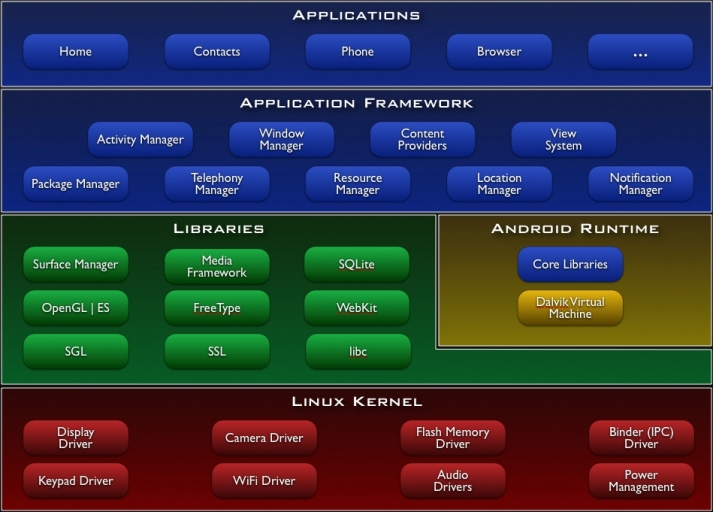
\includegraphics[width=1.5\textwidth, angle=90]{imgs/android_system_architecture.jpg}
	\caption{Architettura di sistema di Android\tm, cortesia di \url{http://developer.android.com}}
	\label{fig:android_system_architecture}
\end{figure}

\subsection*{Linux Kernel}
Il sistema operativo Android (Android OS) \cite{android_dev} si basa sulla versione 2.6 di Linux \cite{linux_kernel} per i servizi centrali di sistema come la sicurezza, la gestione della memoria e dei processi, lo stack di rete ed i modelli dei driver (vedi figura \ref{fig:android_system_architecture}). Il Kernel funziona anche da livello di astrazione tra l'hardware e lo stack di software.
Tutte le applicazioni Android\tm vengono eseguite in processi Linux separati, dopo aver avuto i premessi richiesti dal sistema Linux

\subsection*{Librerie Native Android\tm}
\label{sec:lib_Android}
Le librerie di Android\tm sono principalmente composte da librerie C/C++ della comunit� open source. 
Queste librerie vengono esposte sotto forma di servizi di sistema per i programmatori che vogliano usarli come funzioni senza conoscerne i dettagli implementativi a livello di application framework (vedi figura \ref{fig:android_system_architecture}).
Le librerie principali sono: 
\begin{itemize}
	\item \textbf{Librerie Standard di (ANSI) C}: un implementazione BSD\footnote{Berkley Software Distribution e licenza Apache/MIT che a differenza della licenza GNU non obbliga sviluppatori a ridistribuire i loro codici alla comunit�} della libreria Standard di C (\textit{libc}), ottimizzata per dispositivi basati sul sistema Linux. Alcuni esempi di servizi della libreria sono l'allocazione di memoria, la gestione dell'input/output ecc.
	\item \textbf{Librerie Media}: basate sulle OpenCORE \cite{packetVideo_openCore} di PacketVideo\footnote{PacketVideo � il membro fondatore Open Handset Alliance}, versione open source della libreria CORE\tm  della stessa compagnia. Queste librerie supportano la visualizzazione (playback) e la registrazione  dei formati audio e video ed immagini statiche pi� popolari (MPEG4, H.264, MP3, AAC, AMR, JPG, e PNG).
	\item \textbf{Surface Manager}: gestisce l'accesso al sottosistema di visualizzazione e compone, in modo trasparente all'utente, la grafica 2D con quella 3D di applicazioni multiple.
	\item \textbf{LibWebCore}: un motore per un web browser, che pu� essere usato sia dal browser di Android\tm che da una vista del web incorporata in un applicativo. LibWeb \cite{LibWeb} � una libreria/toolkit per sviluppare applicazioni Web scritte in Perl.
	\item \textbf{SGL}: motore grafico 2D.
	\item \textbf{Librerie 3D}: un'implementazione basata sulle API di OpenGL\footnote{Open Graphics Library} \cite{OpenGL}. Le librerie usano l'acceleratore grafico 3D, dove disponibile, e il rasterizzatore\footnote{Trasformatore di un oggetto grafico dalla sua descrizione vettoriale in una descrizione visuale, vale a dire pixel o punti che possano essere visualizzati su uno schermo o stampati.} altamente ottimizzato per programmi 3D incluso nella distribuzione. OpenGL � un ambiente per sviluppare grafica sia 2D che 3D, interattiva e portabile.
	\item \textbf{FreeType} \cite{FreeType}: rendering di font con tecnologia bitmap e vettoriale 
	\item \textbf{SQLite} un motore per un database relazionale potente e leggero a disposizione di tutte le applicazioni.
	\item \textbf{OpenSSL} \cite{OpenSSL}:  � un insieme di strumenti Open Source che implementano il Secure Sockets Layer (SSL v2/v3) ed i protocolli Transport Layer Security (TLS v1) ed infine una libreria di crittografia generica di ottimo livello.
\end{itemize}



\subsection*{Macchina Virtuale di Android\tm: Dalvik}
\label{sec:dalvik}
Il linguaggio Java\tm \cite{Java}, JDK\footnote{Java Developement Kit} Tools \cite{JDK_Tools} e le librerie Java\tm sono gratuite, mentre la Java Virtual Machine non lo �. Dato che questo andava contro la politica del progetto,  Google\footnote{Dan Bernstein ed il team di sviluppo} ha sviluppato una versione ex-novo della Java Virtual Machine, ad-hoc per Android\tm\footnote{Fino al 2005, non vi erano alternative alla JVM della Sun, poi sono nate OpenJDK              \cite{OpenJDK} e Apache Harmony \cite{Apache_Harmony}}. I problemi principali che il gruppo di sviluppo hanno affrontato sono quelli della durata della batteria e le risorse (memoria e ram) limitate.
\subsubsection{Java\tm e Android\tm}
Normalmente il codice Java\tm viene compilato e poi il bytecode viene eseguito sulla JVM, sotto Android\tm il bytecode viene ricompilato con il compilatore Dalvik (vedi sezione \ref{sec:dalvik}) che produce un Dalvik-bytecode detto Dex, che viene eseguito dal Dalvik VM (vedi figura \ref{fig:Java_vs_Android_compile_exec}).

\begin{figure}
	\centering
	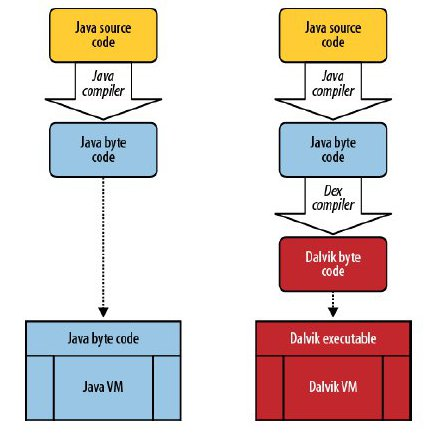
\includegraphics[width=.9\textwidth]{imgs/JVMvsDalvik.jpg}
	\caption{Comparazione del processo di compilazione di un file Java\tm in ambiente Android\tm con quello classico. Immagine cortesia di \cite{Gargenta_android}}
	\label{fig:Java_vs_Android_compile_exec}
\end{figure}

Il processo � automatizzato dall'IDE\footnote{I Developement Environment} (Eclipse\tm o ANT \cite{Apache_Ant}) che si usa.
La distribuzione Java\tm di Android\tm non � standard: � una variante di JSE\tm (Java Standard Edition), in cui le Java AWT e Swing sono state sostituite da Android\tm UI\footnote{User Interface}, appositamente ottimizzate per gli schermi e le schede grafiche di dimensioni ridotte dei dispositivi.
\subsection*{Application Framework}
Questa � la parte della piattaforma che permette di sviluppare applicativi Android\tm, fornendo servizi (sensori, posizionamento, telefonia, Wifi ecc) ed abbondante documentazione in merito. 
\subsection*{Applications}
Le applicazioni sono i programmi sviluppati dal mondo di sviluppatori Android\tm. Questi possono essere sia gi� istallati all'acquisto del dispositivo, sia scaricati dai mercati Android\tm. 
\subsubsection*{APK}
Un applicazione Android\tm � un singolo file, detto APK file. Questi ha tre componenti principali:
\begin{enumerate}
	\item \textbf{Eseguibile Dalvik} Il codice Java\tm compilato come descritto in figura (vedi figura \ref{fig:Java_vs_Android_compile_exec}).
	\item \textbf{Risorse} Tutto cio che � in un applicativo Android\tm, ma non � codice Java\tm: file XML, immagini, audio, video ecc.
	\item \textbf{Librerie} In un applicativo possono essere incluse librerie di codice nativo, ad esempio in C/C++
\end{enumerate} 
\subsection*{Struttura di un Android\tm App}
\label{sec:android_app_structure}
Ogni applicativo per Android\tm deve una determinata struttura di cartelle e file per funzionare. Il file pi� importante � l'AndroidManifest. Questo file funziona da collante e da indice per comprendere le componenti dell'applicativo. Contiene i permessi che ha come applicativo, di interagire con il resto del sistema operativo. \\
Lavorando in ambiente di sviluppo Eclipse SDK \tm, con il plugin per Android\tm SDK Manager, la creazione di un nuovo progetto (Android Project), genera la struttura del programma:
\begin{itemize}
	\item \textbf{src} : codice java 
	\item \textbf{gen} : file auto generati per la gestione delle risorse
	\item \textbf{Android\tm 2.2} (Libreria) : tutta la libreria di Android\tm 
	\item \textbf{assets}: risorse che non vengono auto indicizzate in R
	\item \textbf{bin}: file binario
	\item \textbf{AndroidManifest.xml}
\end{itemize}

\section*{Le componenti principali di un Applicativo Andorid}
\label{sec:android_main_components}
Lo sviluppo di programmi (Java\tm) per applicativi Android\tm � necessariamente vincolato dal fatto che l'interazione dell'utente avviene mediante lo schermo del dispositivo, la durata della batteria � limitata, la capacit� computazionale � ridotta ecc.
Gli sviluppatori di Android\tm hanno creato un framework per sviluppare applicativi, che risolve la maggior parte dei problemi del programmatore. L'impostazione di base del framework � quella della programmazione ad eventi, con un meccanismo di callback (riferimento a un codice) asincrono. 
Le componenti principali sono:
\begin{enumerate}
	\item \textbf{Acitivity}: un'attivit� � la logica che gestisce una schermata singola che l'utente vede. Gli applicativi hanno di solito molteplici activity che permettono all'utente di navigare l'applicativo secondo la sua logica,
	\item \textbf{Intent}: messaggi asincroni inviati tra le componenti principali,
	\item \textbf{Service}: logica dell'applicativo,
	\item \textbf{Content Provider}: interfaccia per lo scambio di dati tra applicativi,
	\item \textbf{Broadcast Receiver}: metodo per gestire chiamate a livello di sistema in modo asincrono,
	\item \textbf{Application Context}: contesto in cui tutta l'applicazione esiste.
\end{enumerate}

\subsection*{Activity}
Ogni applicativo Android\tm ha una \textit{main activity}, che definisce la logica della schermata iniziale.
Nell'ottica di ottimizzare le risorse del dispositivo, le activity sono state progettate in modo da consumare il minimo.
Quando viene lanciata una activity, viene creato un processo Linux, viene allocato dello spazio per gli oggetti UI, costruire oggetti Java\tm a partire dalle definizioni XML (inflation), posizionare oggetti sullo schermo. Per evitare di incorrere in questo costo ogni volta che si ricapita su una schermata, le activity sono state progettate per avere un ciclo di vita, gestito da un activity Manager. Quest'ultimo si occupa di creare, gestire e distruggere le activity, all'occorrenza.
Ogni activity attraversa i seguenti stati (vedi figura \ref{fig:Activity_lifecycle}):
\begin{enumerate}
	\item \textbf{Starting}: l'activity non esiste in memoria. I metodi della classe \texttt{Activity} che permettono di gestire l'evento di creazione di una activity sono \texttt{onCreate()},  \texttt{onStart()} ed \texttt{onResume()} tutti per andare nello stato Running. 
	\item \textbf{Running}: l'activity � sullo schermo e l'utente ci sta interagendo. In ogni dato istante di tempo, pu� esistere solo un'activity in questo stato. Tra tutte le activity, quella nello stato Running ha la massima priorit� per l'utilizzo della risorse, per minimizzare i tempi di risposta all'utente. Il metodo per gestire l'evento � \texttt{onPause} per andare nello stato Paused.
	\item \textbf{Paused}: l'activity � ancora visibile, ma l'utente non vi pu� interagire. Non � uno stato molto comune, perch� date le dimensioni ridotte dello schermo, generalmente le activity occupano tutto lo schermo o niente. Ad esempio quando appare una dialog box su una schermata, la schermata � nello stato Paused. Tutte le activity attraversano questo stato nel momento in cui vengono fermate. Queste activity sono tra quelle a priorit� pi� alta, perch� sono ancora visibili, e la transizione ad un'altra activity deve essere compiuto in modo fluido. Le callback dello stato sono \texttt{onResume()} per tornare nello stato Running e \texttt{onStop()} per andare nello stato Stopped.
	\item \textbf{Stopped}: un'activity si trova in questo stato se non � pi� visibile ma � ancora in memoria. Queste possono essere distrutte oppure tenute in memoria per essere ripristinate nello stato Running. La seconda operazione � molto meno costosa della creazione ex-novo di un'activity. Le callback di questo stato sono le stesse dello stato Starting ed il metodo \texttt{onDestroy()} per andare nello stato Destroyed. 
	\item \textbf{Destroyed}: l'activity viene rimossa dalla memoria, se l'Activity Manager decide che questa non verr� usata per abbastanza tempo da rendere pi� conveniente la ricreazione della stessa al suo trattenimento in memoria.
\end{enumerate}

\begin{figure}
	\centering
	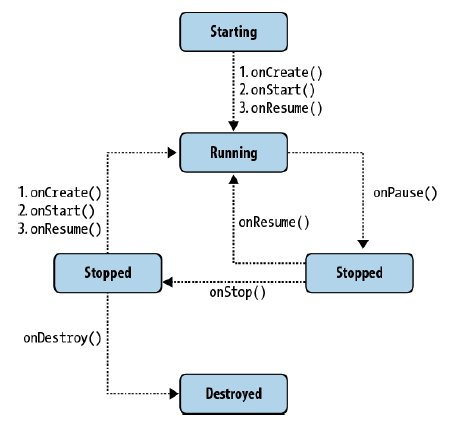
\includegraphics[width=.9\textwidth]{imgs/ActivityLifeCycle.jpg} 
	\caption{Ciclo di vita di una Activity, cortesia di \cite{Gargenta_android}}
	\label{fig:Activity_lifecycle}
\end{figure}

\subsection*{Intent}
Le Intent possono essere viste, come dice il nome, delle intenzioni di creare Activity che un mittente comunica.
Queste potrebbero essere usate da un'Activity per creare un'altra activity, oppure per far partire un servizio o per inviare un messaggio in broadcast. Questi possono essere espliciti se il mittente dichiara il ricevente, o impliciti se il mittente dichiara solo il tipo di ricevente. Nel secondo caso ci potrebbero essere dei riceventi in competizione per l'esecuzione del messaggio, ed il sistema lascia all'utente la scelta del esecutore.

\subsection*{Servizi}
Questi non hanno un interfaccia utente ed il loro ciclo di vita o esecuzione � trasparente a chi utilizza il sistema. Il ciclo di vita di un servizio � molto semplice: 
inizialmente il servizio viene creato, ed il suo primo stato � detto Starting. Da qui le callback da usare per intercettare la transizione in Running sono \texttt{onCreate()} ed \texttt{onStart()}. Dallo stato Running con la callback \texttt{onDestroy()} il servizio va nell'ultimo stato in cui si pu� trovare: Destroyed.\\
I service che sono particolarmente impegnativi dal punto di vista computazionale dovrebbero essere eseguiti su un proprio thread, eseguibile in background, e non quello della UI, in modo da non rallentare l'interfaccia grafica.
\subsection*{Content Provider}
Android\tm, per ragioni di sicurezza, esegue ogni applicativo nella propria "`sandbox"' compartimento stagno, in modo da confinare i dati usati da un programma a quest'ultimo. Mediante gli Intent � possibile scambiare piccole quantit� di dati tra applicativi diversi, la condivisione di quantit� ingenti di dati persistenti viene fatta tramite i 
Content Provider. Per facilitare il compito questo componente aderisce all'interfaccia CRUD: il Content Provider � interfacciato ad una base di dati ed implementa i metodi \texttt{insert()}, \texttt{delete()}, \texttt{update()}, \texttt{query()}.

\begin{figure}
	\centering
	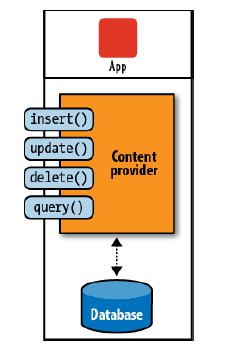
\includegraphics[width=.45\textwidth]{imgs/CRUD.jpg}
	\caption{ CRUD di un Content Provider, cortesia di \url{http://developer.android.com}}
	\label{fig:coInterfacciantent_provider}
\end{figure}

\section*{Broadcast Receiver}
Implementazione del pattern Observer (tipo particolare del protocollo Publish/Subscribe) in cui c'� un servizio di prenotazione su un certo evento. Un programma si registra al servizio e nel momento in cui viene lanciato l'evento per il quale si � registrato, il codice viene lanciato. Il sistema operativo lancia eventi in broadcast in continuazione: il sistema � stato avviato, la batteria � scarica, un sms � in arrivo ecc. Ciascuno di questi eventi scatena il lancio dei programmi registrati, o per usare il nome del pattern, i programmi che osservavano l'evento.  
\section*{Application Context}
\label{sec:application_context}
Il contesto di un'applicativo Android\tm � l'ambiente in cui i processi con tutti le componenti vengono eseguiti. Il ciclo di vita di un contesto parte con la sua creazione al lancio dell'applicativo, e termina nel momento in cui questi viene terminato. Per avere un riferimento al contesto � sufficiente chiamare \texttt{Context.getApplicationContext()} oppure \texttt{Activity.getApplication()}


%\section*{Intefaccia Utenti (UI)}\TODO{Completare}
%\url{http://developer.android.com/guide/topics/ui/index.html}
%\subsection*{Layout XML}
%\label{sec:layout}
%\subsection*{Eventi di Input}
%
%\subsection*{Menu}
%\label{sec:menu}
%Per default ogni Activity ha un menu di opzioni o azioni, a cui l'utente pu� accedere premendo un taso fisicamente disegnato sullo schermo. 
%\subsection*{Barra delle Azioni}
%\subsection*{Dialoghi}

%\myChapter{Ringraziamenti}
prof Angelo Sabatini per avermi accolto a braccia aperte nel suo team ed avermi sostenuto nei momenti pi� difficili
Andrea Mannini per essere stato sempre presente durante l'anno di lavoro
Ing Vincenzo Genovese
Charlie Roche per essere il mio mentore di programmazione, basket, freesby, bigliardo, cinema e amico.
Tommaso Baviera 
Andrea Guitto
Barbara Marini

Sara Porporato $\heartsuit \heartsuit \heartsuit$


%--------------------------------------------------------------
%	Extras
%--------------------------------------------------------------
\chapter*{@Todo List}
Instructions on how to use this list: instead of writing a TODO right in the middle of the thesis, I should write it in this list and refer to it with a label such as \verb|\label{TODO:keyword}|
where keyword has to be unique.
\begin{itemize}
	\item \sout{Stop using the $eng\_to\_ita$ file. Define a word the first time and use it with an acronym if possible.}
	\item \sout{Tableofcontents: make parts centered, chapters bold.}
	\item Write all non Italian words in italic (Ctrl+k) which is ironc! 
	\item Collect all TODOs. 
	\item Insert relevant words in TeXnicCenter's dictionary so that I can notice any typing mistakes.
	\item Eliminate repetitions.
	\item Uniformare immagini: dimensioni, didascalia, posizione testo, colore, tipo di disegno (schizzo, preciso ...).
	\item Uniformare tabelle: dimensioni, didascalia, posizione testo, colore, tipo di disegno (schizzo, preciso ...).
	\item Inserire elenco di figure e tabelle 
\end{itemize}

%--------------------------------------------------------------
\bibliographystyle{IEEEtran}
\bibliography{biblio}
%\printglossaries
%\addcontentsline{toc}{chapter}{Glossary}
\end{document}
%------------------------------------	--------------------------
	